\documentclass{report}
\usepackage{amsthm,amssymb}
%\usepackage{amsmath} %already loaded by mathtools
\usepackage{titlesec}%required for \titleformat
\usepackage{mathtools}%automatically loads amsmath and is required for \defeq macro
\usepackage{tcolorbox}%required for \definecolor
\usepackage[colorlinks=true, linkcolor=purple]{hyperref}
\usepackage{geometry}
\usepackage[inline]{enumitem}%for "enumerate*" (i.e. horizontal lists)
\usepackage{ifthen}%for "ifthenelse"
\usepackage[twoside]{fancyhdr}
\usepackage{lastpage}
\usepackage{datetime2}
\usepackage{tocloft}
\usepackage[backend=biber]{biblatex}

\setlength{\headheight}{18.0pt}

\addbibresource{test.bib}
%\addbibresource{Primo_BibTex_Export.bib} 

\newcommand{\listdefinitionsname}{\Large List of definitions}
\newlistof{definitions}{dfn}{\listdefinitionsname}

\newcommand{\listofabbreviationsname}{\vspace{-1.2em}\Large List of Abbreviations\vspace{-1.5em}}
\newlistof{abbreviations}{abf}{\listofabbreviationsname}
\newcommand{\addAbbrev}[2]{
    \addcontentsline{abf}{section}{#1 \hspace{1em} - \hspace{1em} #2}
}

\geometry{
    a4paper,
    twoside,
    inner=30mm,
    outer=40mm,
    bottom=15mm,
    top=20mm,
    marginparwidth = 30mm,
    marginparsep = 5mm
}

\titleformat{\chapter}[display]{\bfseries\Large} % format
{\fontfamily{phv}\selectfont\scshape Chapter \thechapter} % label
{1ex} % sep
{   \fontfamily{phv}\selectfont
    \bfseries\huge\centering
} % before-code
[\vspace{-0.7cm}] % after-code

\titleformat{\section}[display]{\Large} % format
{} % label
{-0.2cm} % sep
{   \fontfamily{phv}\selectfont \scshape\thesection\quad 
} % before-code
[\vspace{-0.2cm}] % after-code

\definecolor{purple2}{HTML}{660099}
\definecolor{rhoda}{HTML}{0000B7}
\definecolor{tanita}{HTML}{5173BD}
\definecolor{yellow}{HTML}{FCF434}
\definecolor{purple}{HTML}{9C59d1}
\definecolor{darkgray}{HTML}{2C2C2C}
\definecolor{lightgray}{HTML}{C2C2C2}

%Highlight
\newcommand{\purplebf}[1]{\color{purple}\textbf{#1 }\color{black}}
\newcommand{\graybf}[1]{\color{darkgray}\textbf{#1 }\color{black}}
\newcommand{\bigemph}[1]{\fontfamily{qag}\selectfont\color{darkgray}\textbf{#1 }\color{black}\normalfont}

\newcommand{\defeq}{\vcentcolon=}
\newcommand{\eqdef}{=\vcentcolon}
\newcommand{\defaq}{\vcentcolon\Leftrightarrow}
\newcommand{\sledom}{\Relbar\joinrel\mathrel{|}}
\renewcommand{\AA}{\mathbb{A}}
\newcommand{\KK}{\mathbb{K}}
\newcommand{\NN}{\mathbb{N}}
\newcommand{\RR}{\mathbb{R}}
\newcommand{\CC}{\mathbb{C}}
\newcommand{\ZZ}{\mathbb{Z}}
\DeclareMathOperator{\Erf}{Erf}
\DeclareMathOperator{\nicht}{nicht}
\DeclareMathOperator{\Successor}{S}
\DeclareMathOperator{\varS}{var}
\DeclareMathOperator{\TA}{TA}
\DeclareMathOperator{\frei}{frei}

\DeclareMathOperator{\propM}{Prop} % for example in boolean algebra
%\DeclareMathOperator{\gdw}{\quad:gdw\quad}

\newif\ifSimplifiedVersion
%\SimplifiedVersiontrue

%%\newtheorem{name}[counter]{Printed output}
\newcounter{defcount}[chapter]
\renewcommand{\thedefcount}{Definition \theHchapter.\arabic{defcount}}

\newtheorem{defi}[defcount]{}
\newcommand{\defin}[2]{
%    \begin{defi}
%        \addcontentsline{dfn}{section}{\protect\numberline{\thedefi} #1}
%        \textbf{\fontfamily{txtt}\selectfont{#1}:} \normalfont \color{black}
%        #2
%        \thedefcount
%    \end{defi}

    \ifSimplifiedVersion
        #1
    \else 
        \color{rhoda}   
        \begin{defi}
            \addcontentsline{dfn}{section}{\protect{{\thedefi \hspace{5px} #1}\hspace{-4px}} } 
            \color{tanita}\textbf{\normalfont\fontfamily{txtt}\selectfont{\textbf{#1}}: }%
            \normalfont\color{black}
            #2
        \end{defi}
        \color{black}
    \fi
}

\newcommand{\outernote}[1]{
    \marginpar[\raggedleft #1]{\raggedright #1}
}

%\newtheorem{notes}[]{Bemerkung}
\newcommand{\note}[2]{
    \ifSimplifiedVersion
        Bem: #1 - #2

    \else 
        \color{rhoda}   
        %\begin{notes}
            \noindent Note\fontfamily{txtt}\selectfont{#1}: \normalfont\color{black}
            #2

        %\end{notes}
        \color{black}
    \fi
}
\newcounter{propcount}[chapter]
\renewcommand{\thepropcount}{Theorem \theHchapter.\arabic{propcount}}

\newtheorem{propo}[propcount]{}
\newcommand{\prop}[3]{
    %Input: 1-Name, 2-statement, 3-proof
    \stepcounter{corollcount}
    \ifSimplifiedVersion
        Prop: #1 - #2

    \else 
        \color{rhoda}   
        \begin{propo}
            \color{tanita}\textbf{\normalfont\fontfamily{txtt}\selectfont{\textbf{#1}}: }\normalfont\color{black}
            #2
            \ifx\foo#3\foo
            \else
                \begin{proof}
                    #3%\vspace{5pt}
                \end{proof}
            \fi
        \end{propo}
        \color{black}
    \fi
}
\newcounter{lemmacount}[chapter]
\renewcommand{\thelemmacount}{Lemma \theHchapter.\arabic{lemmacount}}

\newtheorem{lemmata}[lemmacount]{}
\newcommand{\lemma}[3]{
    %Input: 1-Name, 2-statement, 3-proof
    \ifSimplifiedVersion
        Lemma: #1 - #2

    \else 
        \color{rhoda}   
        \begin{lemmata}
            \color{tanita}\textbf{\normalfont\fontfamily{txtt}\selectfont{\textbf{#1}}: }\normalfont\color{black}
            #2
            \ifx\foo#3\foo
            \else
                \begin{proof}
                    #3%\vspace{5pt}
                \end{proof}
            \fi
% legacy: throws errror on listings in #3
%            \ifthenelse{\equal{#3}{}}{}{
%                %\vspace{-5pt}
%                \begin{proof}
%                    #3\vspace{5pt}
%                \end{proof}
%            }
        \end{lemmata}
        \color{black}
    \fi
}

\newcounter{corollcount}[chapter]
\renewcommand{\thecorollcount}{Corollary \theHchapter.\arabic{corollcount}}

\newtheorem{corollary}[corollcount]{}
\newcommand{\coroll}[1]{
    \addtocounter{corollcount}{-1}
    %Input: 1-Statement
    \ifSimplifiedVersion
        Cor: #1

    \else 
        \color{purple}   
        \begin{corollary}
            \color{black}\normalfont#1\vspace{-5px}
        \end{corollary}
        \color{black}
    \fi
}

\newcounter{excount}[chapter]
\renewcommand{\theexcount}{\theHchapter.\arabic{excount}}
\newtheorem{example}[excount]{Example}
\newcommand{\bsp}[2]{
    \ifSimplifiedVersion
        Bsp(#1): #2

    \else 
        %\color{purple}   
        \begin{example}
            \fontfamily{txtt}\selectfont{#1}: \normalfont\color{black}
            #2
        \end{example}
        \color{black}
    \fi
}


\newcommand*{\claimproofname}{proof of claim.}
\newenvironment{claimproof}[1][\claimproofname]{\vspace*{-10px}\begin{proof}[#1]\renewcommand*{\qedsymbol}{\(\boxtimes\)}}{\end{proof}}

\begin{document}

\fancypagestyle{plain}{}
\pagestyle{fancy}   %needed for changing headers/footers
\fancyhf{}          %cleares headers and footers
\fancyhead[LE,RO]{\small\rightmark} 
\fancyhead[LO,RE]{Logic Lecture Notes 2024W}
\fancyfoot[C]{}
\fancyfoot[LO,RE]{\fontfamily{cmtt}\small\color{gray}J.Petermann: LogicNotes [V0.2-\today{ }at \DTMcurrenttime] }% old: \href[]{https://creativecommons.org/licenses/by-nc-nd/3.0/de/}{\color{gray}CC BY-NC-ND 3.0 DE}
\fancyfoot[LE,RO]{Seite \thepage \hspace{3pt}von \pageref*{LastPage}}

\begin{center}
    \fontfamily{qag}\selectfont
    \Huge\textbf{Lecture notes\\ Einführung in die Logik 2024W}\\
    \normalfont
\end{center}
\begin{center}
    \framebox[14cm]{\parbox{\dimexpr\linewidth-2\fboxsep-2\fboxrule}{
    This is a summary of the material discussed in the lecture "Mathematische Logik". 
    It is still a work in progress and there \textbf{may me mistakes} in this work. 
    If you find any, feel free to let me know and I will correct them\\\hspace{10px}
    The content of this script is intended for educational purposes only. 
    It relies on the book \cite{EndertonHerbertB2001AMIt} for which all rights belong to their respective 
    owners and I do not claim ownership over this content. 
    However the \LaTeX code I wrote is entirely my own work and is provided to you by the \href[]{https://choosealicense.com/licenses/mit/}{\color{gray}MIT-Licence}.
    Dieses Skript ist noch nicht vollständig und wird regelmäßig aktualisiert.}
}
\end{center}

\setlength{\cftbeforetoctitleskip}{0em}
\setlength{\cftaftertoctitleskip}{0em}
\tableofcontents
\listofabbreviations
\newpage

    
\chapter{Propositional logic}
\addAbbrev{prop.}{propositional}
\defin{Language of PL}{
The Language \outernote{Language} of Propositional logic is a set containing
    \begin{itemize}
        \item logical symbols: consisting of the \graybf{sentential connective} symbols $\lnot, \land, \lor, \to, \leftrightarrow$ and parenthesis $(,)$
        \item non-logical symbols: $ A_1, A_2,A_3,\dots$ (also called sentential atoms, variables)
    \end{itemize}
    from which we assume (for unique readability) that no symbol is a finite sequence of any other symbols.
}
\note{}{
    \begin{enumerate}
        \item The role of the logical symbols doesn't change, the sentential atoms we see as variables, they function as placeholders or variables.
        \item we assumed the set of non-logical symbols is countable, for most of our conclusions you could use any set of prop. atoms of any size
    \end{enumerate}
}
\addAbbrev{exp.}{expression(s)}
\defin{Expression / prop. sentence}{An \graybf{expression}\outernote{expression} is a any finite sequence of symbols
    We define \graybf{grammatically correct exp.} recursive
    \begin{enumerate}
        \item every prop. atom is a prop. sentence
        \item if $\alpha, \beta$ are prop. sentences, then also $\lnot \alpha, \alpha \land \beta, \alpha \lor \beta, \alpha \to \beta, \alpha \leftrightarrow \beta$
        \item nothing else (in particular $\varnothing$ is not a prop. fla.)
    \end{enumerate}
    and call them \graybf{prop. sentences} or \graybf{prop. fla.}\outernote{prop. fla.}\outernote{prop. sentence}
    Equivalently stated every prop. sentence is built up by applying finitly many formula building operations on atoms and the prop. sent. returned from building operations.
    \[\mathcal{E}_\lnot, \mathcal{E}_\lnot(\alpha) \defeq (\lnot \alpha) \text{ for any prop. fla. $\alpha$ and similarly for } \mathcal{E}_\land,\mathcal{E}_\lor \mathcal{E}_\to, \mathcal{E}_\leftrightarrow\]
    This allows us to symbolize the \graybf{expression tree} (Here for example for $((\lnot(A_1\to A_2))\lor A_3))$
    \begin{figure}[h]
        \centering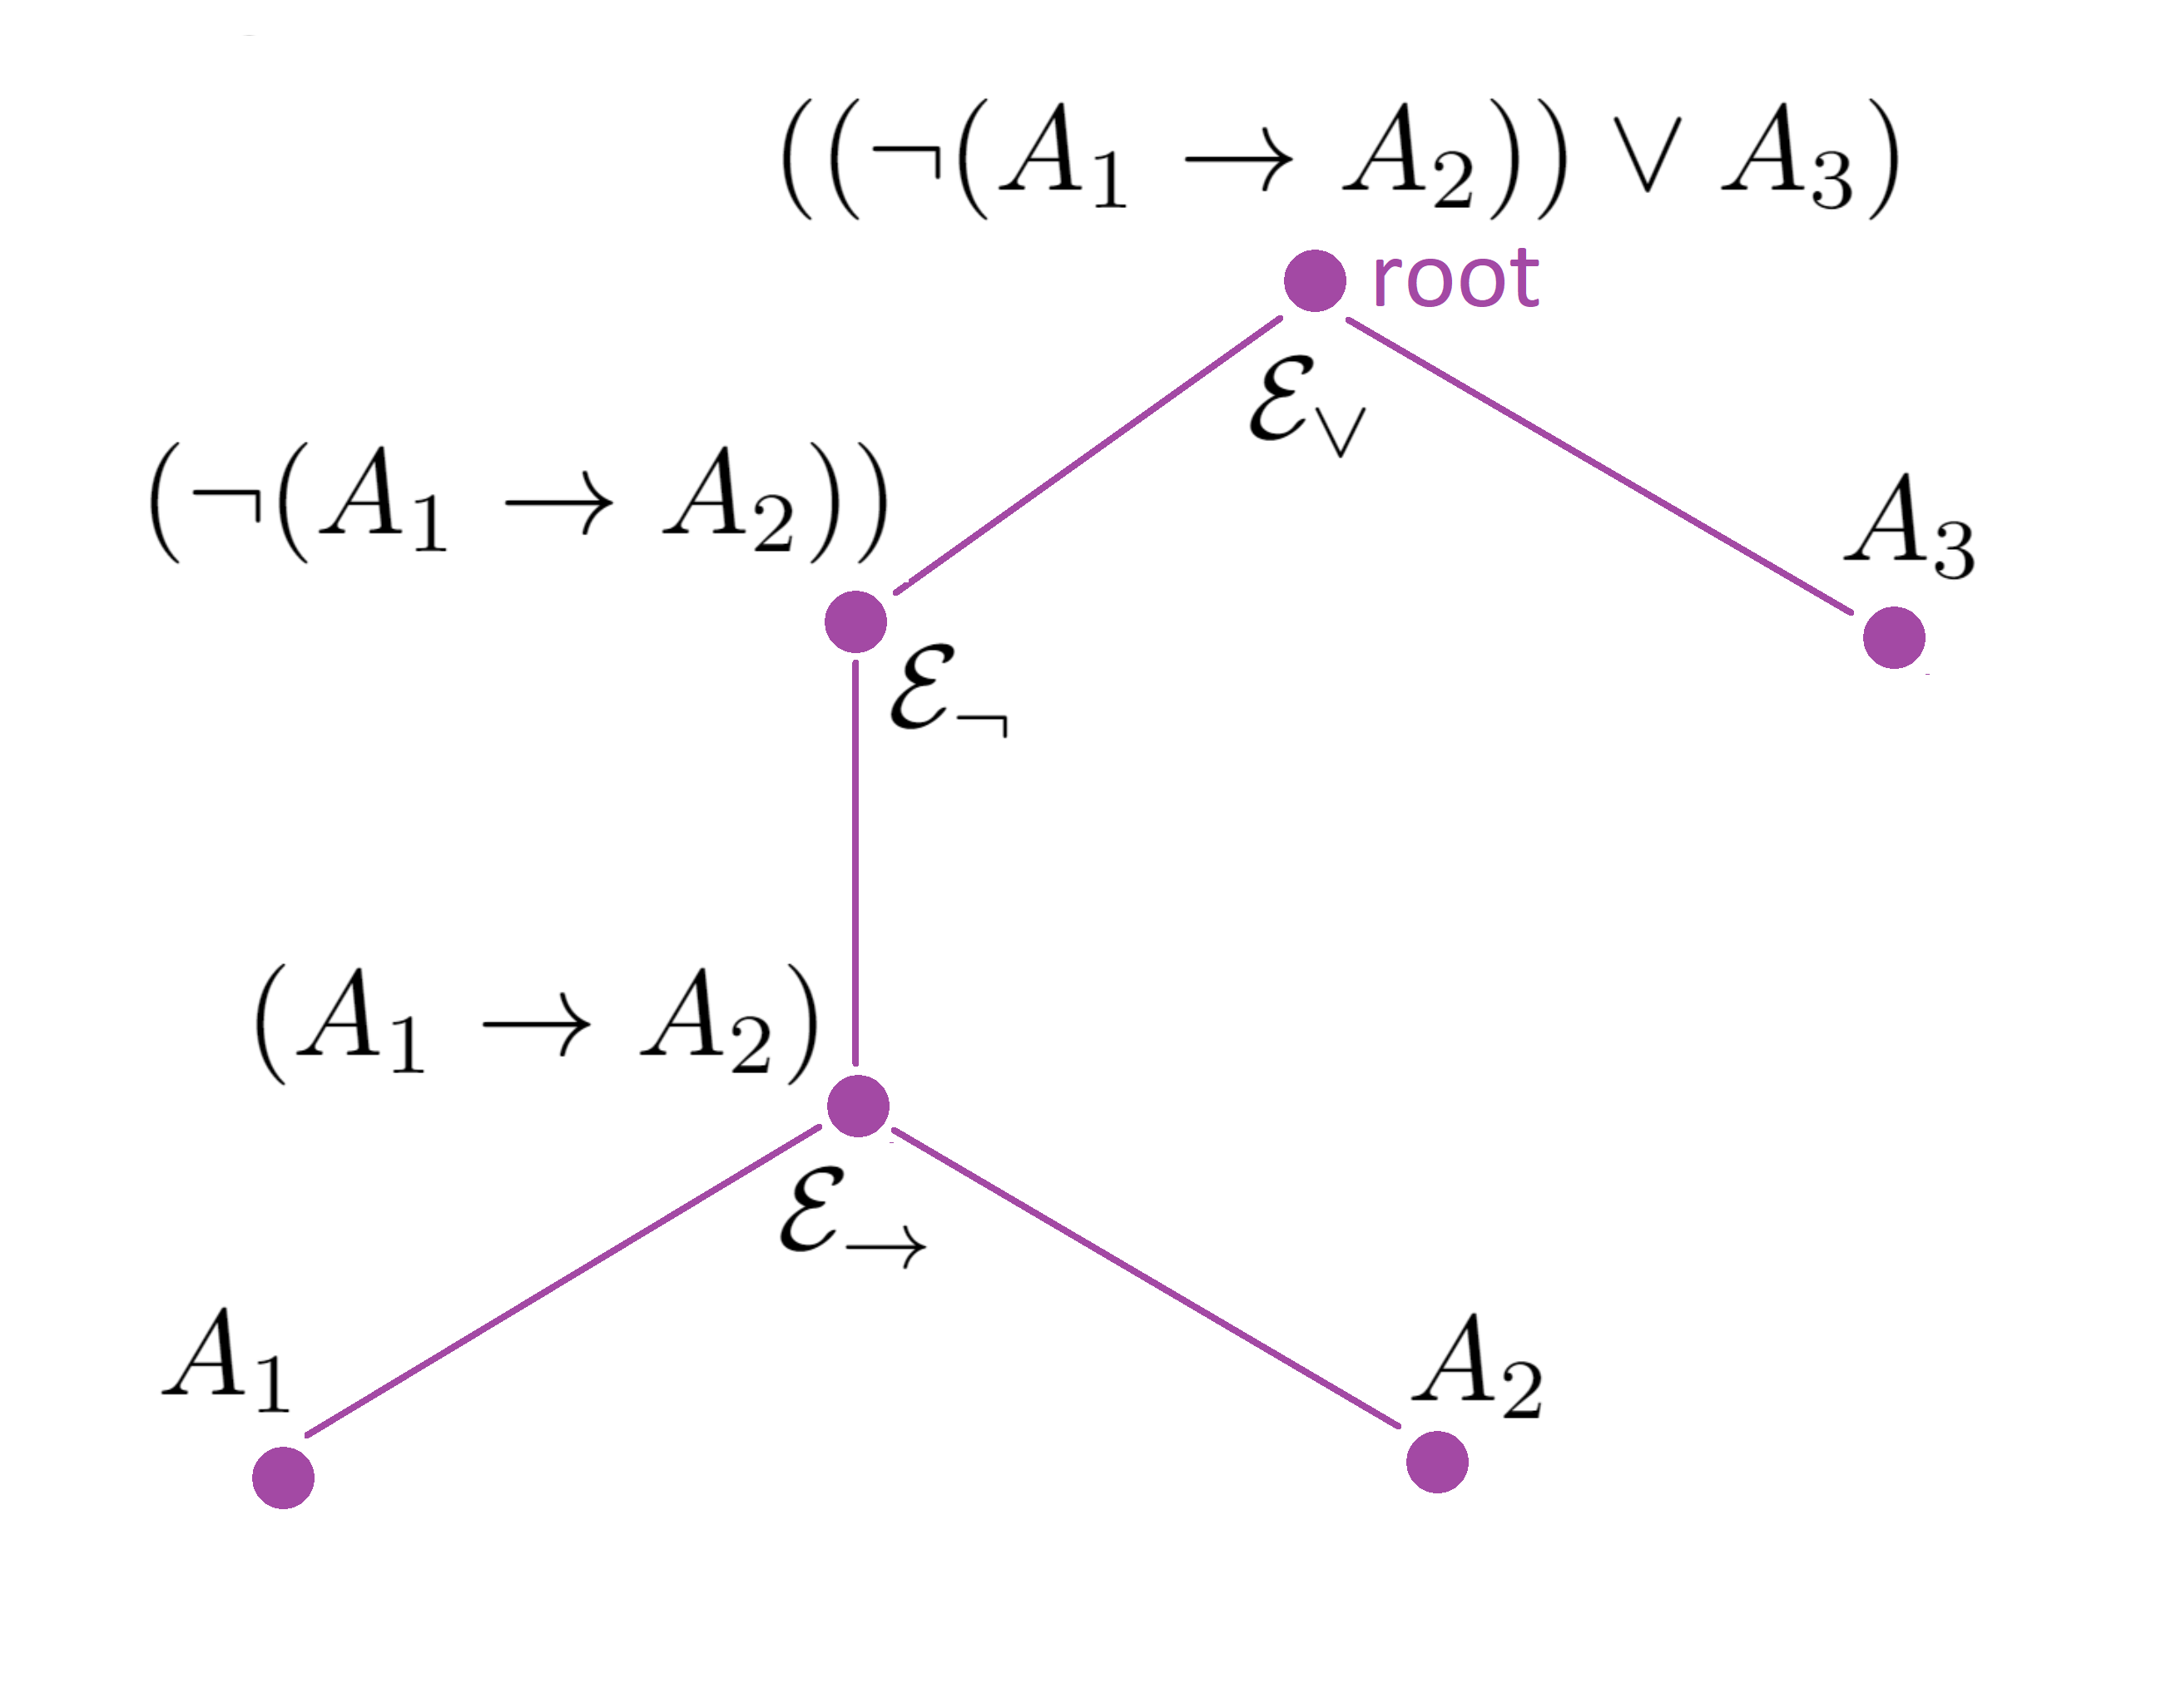
\includegraphics[width = 6cm]{1-extree.png}
    \end{figure}
    
}
We will return to these construction trees in \ref{section_parsingalg}, where we answer the question of what 
truth value a given prop. sentence might have.
\newpage
\defin{Construction sequence}{
    Given a prop. sentence $\alpha$ a \graybf{construction sequence}\outernote{construction sequence} of $\alpha$ is a finite sequence $\left\langle \alpha_1,\dots \alpha_{n-1},\alpha\right\rangle$ such that for all $i\leq n$
    the following holds
    \begin{itemize}
        \item $\alpha_i$ is a sentential atom
        \item or $\alpha_i= \mathcal{E}_\lnot(\alpha_j)$ for some $j< i$
        \item or $\alpha_i= \mathcal{E}_{\square }(\alpha_j,\alpha_k)$ for some $j,k<i$ and $\square\in\{\land,\lor,\to,\leftrightarrow\}$
    \end{itemize}
}
\defin{}{Let $S$ be a set. We say $S$ is \graybf{closed}\outernote{closure} under an $n$-ary operational symbol $f$
    iff for all $s_1,s_2,\dots s_n\in S$ it holds $f(s_1,s_2,\dots s_n)\in S$ 
}
\addAbbrev{sent.}{sentence(s)}
\addAbbrev{seq.}{sequence}
\noindent\graybf{Induction principle:} Suppose $S$ is a set of prop. sentences
containing all prop. atoms and closed under the 5 formula building operations, 
then $S$ is the set of all prop. sentences.
\begin{proof}
    let $PS = \text{set of all prop. sent.}$
    \begin{itemize}[leftmargin=2cm]
        \item[$S\subseteq PS$:] is clear
        \item[$S\supseteq PS$:] let $\alpha\in PS$ then $\alpha$ has a construction seq. $\left\langle \alpha_1,\dots \alpha_{n-1},\alpha\right\rangle$ and $\alpha_1\in S$
        lets assume that $\alpha_i$ for $i\leq k<n$ is in $S$ then $\alpha_{k+1}$ is either an atom and therefore in $S$ or its obtained by one of the formula building operations 
        from the 
        and therefore $\alpha_{k+1}\in S$
    \end{itemize}
\end{proof}
\addAbbrev{TA}{truth assignment}
\section{Truth assignments}
%We will answer the question when does a prop. sent. follow from other prop. sentences.
The interpretation of a prop. atom is either true or false, denoted by $0 / 1$ or $T / F$ or $\top / \bot$. 
A truth assigment is simply any map $\nu:S\mapsto \{0,1\}$, where $S$ is a map of propositional atoms. 
Our goal is going to be to extend any truth assigment $v$ to a function $\overline{v}: \overline{S}\mapsto \{0,1\}$, where $\overline{S}$ is the closure
of $S$ under the $5$ fla. building operations. 
\addAbbrev{fla.}{formula}
\addAbbrev{TV}{truth value}
\defin{Truth assignment}{\label{TAConditions}
Let $\{0,1\}$ be the set of truth values. \outernote{Truth assigment} A truth assignment \outernote{TA}(TA) for a set $S$ of prop. atoms is a map $\nu:S\to\{0,1\}$}
We now want to extend $\nu$ to $\overline{\nu}: \overline{S}\to \{0,1\}$, where $\overline{S}$ is the closure of $S$ under the 5 fla. building operations such that
for all propositional atoms $A\in S$ and propositional formulas $\alpha,\beta$ in $\overline{S}$
\begin{enumerate}
    \item $\overline{\nu}(A) = \nu(A)$ 
    \item $\overline{\nu}(\lnot \alpha) = 1- \nu(\alpha)$ 
    \item $\overline{\nu}(\alpha \land \beta) = \begin{cases}
        1 & \text{iff } \overline{\nu}(\alpha) = 1 = \overline{\nu}(\beta)\\
        0 & \text{otherwise}
    \end{cases}$
    \item $\overline{\nu}(\alpha \lor \beta) = \begin{cases}
        1 & \text{iff } \overline{\nu}(\alpha) = 1 \text{ or } \overline{\nu}(\beta) = 1\\
        0 & \text{otherwise}
    \end{cases}$
    \item $\overline{\nu}(\alpha \to \beta) = \begin{cases}
        1 & \text{iff } \overline{\nu}(\alpha) = 0 \text{ or } \overline{\nu}(\beta) = 1\\
        0 & \text{otherwise}
    \end{cases}$
    \item $\overline{\nu}(\alpha \leftrightarrow \beta) = \begin{cases}
        1 & \text{iff } \overline{\nu}(\alpha) =  \overline{\nu}(\beta)\\
        0 & \text{otherwise}
    \end{cases}$
\end{enumerate}
We also want the extention to be unique, that is
\prop{Unique readability}{\label{extendetTruthAss}\label{ThrmUniqueExt}
    For all TA $\nu$ for a set $S$ $\exists ! \overline{\nu}:\overline{S}\to\{0,1\}$ satisfying the above properties}{}
We will proof this later\\

\defin{Satisfaction}{A TA $\nu$ satisfies\outernote{satisfy} a prop. sent. $\alpha$ 
    if $\overline{\nu}(\alpha)=1$ (that is, provided that everery atom of $\alpha$ is in the domain of $\nu$). 
    We call $\alpha$ satisfiable\outernote{satisfiable} if there exists a TA that satisfies it.}
\defin{Tautological implication}{\outernote{taut. implication $\models$}\addAbbrev{taut.}{tautological}
    Let $\Sigma$ be a set of prop. sent. and $\alpha$ a prop. sent. then we say:
    $\Sigma$ tautologically imlies $\alpha$ if for all TA that satisfy $\Sigma$, $\alpha$ is also satisfied and we write $\Sigma\models \alpha$.
    If $\Sigma = \{\beta\}$, we simply write $\beta \models \alpha$ If $\Sigma = \varnothing$ then $\alpha$ is called a \graybf{tautology} and we write $\models \alpha$ instead of $\varnothing \models \alpha$ \\
    $\alpha, \beta$ are called \graybf{tautologically equivalent} iff $\alpha\models \beta$ and $\beta\models \alpha$, we then write $\alpha \sledom \models \beta$
}

\note{}{In other words, tautological implication $\Sigma\models \alpha$ means that you can not find a TA, that satisfy all members of $\Sigma$ but not $\alpha$.
    A tautology is satisfied by every TA. Suppose there is no TA that satisfies $\Sigma$, then we have $\Sigma \models \alpha$ for every prop. sent. $\alpha$}
\bsp{}{$\{\lnot A \lor B\} \sledom \models A \to B$ }
\note{}{In order to check if a prop. sent. is satisfiable we need to check $2^N$ TAs, where $N=\text{\# of atoms}$. It is unknown if this can be done by an algorithm in polynomial time. Answering this 
    would settle the debate whether $P=NP$}

However we can find a way to reduce satisfiability of an infinite set $\Sigma$ of prop. sent. to all finite subsets of $\Sigma$.
There later will be a more elementary proof of the compactness theorem, this proof is not part of the exam.
\prop{Compactness theorem}{Let $\Sigma$ be an infinite set of prop. sent. such that 
    \begin{equation}\tag{finite satisfiability}
        \forall \Sigma_0 \subseteq \Sigma, \Sigma_0 \text{finite} \exists \text{ TA satisfying every member of } \Sigma_0
    \end{equation}
    then there is a TA satsfying every member of $\Sigma$.}
{
    using topology: We have our infinite set of prop. sent. which satisfies above condition. One way to look at TA is as a sequence of $0$ and $1$.
    Let $\mathcal{A} = \{A_0, A_1,\dots\}$ be the set of all prop. atoms. We are going to identify the truth assignments on $\mathcal{A}$
    with elements in $\{0,1\}^\mathcal{A}\defeq \{f: \mathcal{A}\to \{0,1\}\}$ (the set of all TAs)
    This is a topological space with product topology, on which we will define
    the basic open sets (called cylinders) by:
    $ U\subseteq \{0,1\}^\mathcal{A}$ is a cylinder, if it holds $p_n(U) = \{0,1\}$for all but finite many $n$, where $p_n$ is the $n$-th projections.
    This means $U$ is a cylinder if the truth values of its elements are at finitely many places fixed, and are arbitrary on everything else.
    
    
    Note: This basic open sets are also closed.
    We now define the open sets as unions of basic open sets.
    The idea is to use Tychonoffs Theorem which tells us that $\{0,1\}^\mathcal{A}$ is compact. i.e.
    the intersection of a family of closed subsets w/ the finite intersection property (FIP) is non-empty
    finite intersection property means the intersection of finitly many sets is non-empty.

    For $\alpha \in \Sigma$ let $T_\alpha \subseteq \{0,1\}^\mathcal{A}$ be the set of TA that satisfy $\alpha$.
    This $T_\alpha$ is a finite union of cylinders, bc. it only depends on finitly many assigments, hence $T_\alpha$ is closed.
    For the family $\{T_\alpha: \alpha\in\Sigma\}$ of closed sets we have (FIP). Tychonoff tells us, 
    that $\bigcup_{\alpha\in\Sigma}{T_\alpha}\neq \varnothing$ so there is a TA satisfying $\Sigma$.}
    
    For a list of tautogies: useful might be book p. 26-27
\section{A parsing algorithm}\label{section_parsingalg}
To prove \ref{extendetTruthAss} We essentially need to show that we have enough parenthesis to make the reading of a prop. sent. unique.
That is given a TA $v$ there is at most one truth value we can assign to a prop. sent.
\addAbbrev{w/}{with}
\lemma{}{Every prop. sent. has the same number of left and right parenthesis.}{
    Let $M = \text{set of prop. sent. w/ \# left parenthesis = \# right parenthesis}$ and \\
    $PS = \text{set of all prop. sent.}$
    We have $M\subseteq PS$. Since atoms have no parenthesis, they are in $M$. we just need to show that
    $M$ is closed under the 5 construction operations.\\
    $\mathcal{E}_{\lnot} = (\lnot \alpha)$ \dots
}
\newpage
\lemma{}{No proper initial segment of a prop. sent. is itself a prop. sent.}{\label{NoPropIni}
    Let $\alpha = \alpha_1\alpha_2\dots \alpha_n$ be a prop. sent. By proper initial segment we understand $\beta = \alpha_1\dots \alpha_i$ for $1\leq i<n$.    
    We will prove that every proper initial segment has an excess of left parenthesis, then we use the previous lemma.
    Let $PS = \text{set of all prop. sent.}$ and \\
    $PF = \text{set of prop. sent. s.t. no proper initial segment has \# left parenthesis = \# right parenthesis}$, 
    we will prove that these sets are the same.\\
    Let $\alpha \in PF$. By induction over the fla. building operations
    \begin{itemize}
        \item Atoms: since the empty sequence is no prop. sent. they have no proper initial segment.
        \item If the above is true for $\alpha, \beta$ then the proper initial segments of $(\lnot \alpha)$ are of the form
        \begin{itemize}
            \item[] $(\lnot \alpha$
            \item[] $(\lnot \alpha'$ where $\alpha'$ is a propper initial segment of $\alpha$
            \item[] $($ \qquad or
            \item[] $(\lnot$
        \end{itemize}
        Therefore $\mathcal{E}_\lnot$ preserves this property and 
        under $\mathcal{E}_\land, \mathcal{E}_\lor, \mathcal{E}_\to, \mathcal{E}_\leftrightarrow$ this is also the case.
    \end{itemize}
}
\subsubsection*{Parsing algorithm}
We now give a parsing algorithm procedure. For input we take some expression $\tau$ and the algorithm will determine if $\tau$ is a prop. sent.
If so, it will generate a unique construction tree (in form of a rooted tree) for $\tau$. (i.e. the construction tree gives us a unique readability)
That there is a unique way to perform the algorithm is implied by \ref{NoPropIni}
\begin{enumerate}
    \item[0.] create the root and label it $\tau$
    \item HALT if all leaves are labled w/ prop. atom and return: "$\tau$ is a prop. sent."
    \item select a leaf of the graph which is not labled w/ prop. atom
    \item if the first symbol of label under consideration is not a left parenthesis, then halt and return: "$\tau$ is not a prop. sent."
    \item if the second symbol of the label is "$\lnot$" then GOTO 6.
    \item scan the expression from left to right\\
    if we reach a proper initial segment of the form\addAbbrev{lp / rp}{left / right parenthesis} "$(\beta$" where $\# lp(\beta) = \#rp(\beta)$ and $\beta$ is followed by one of thesection
    $\land,\lor,\to,\leftrightarrow$ and the remainder of the expression is of the form $\beta')$, where $\# lp(\beta') = \#rp(\beta')$
    \begin{itemize}
        \item [Then:] create two child nodes (left,right) to the selected element and label them (left $\defeq \beta$, right $\defeq \beta'$) GOTO 1.
        \item [Else:] HALT and return "$\tau$ is not a prop. sent."
    \end{itemize}
    
    \item if the expression is of the form $(\lnot \beta)$ where $\# lp(\beta) = \#rp(\beta)$
    \begin{itemize}
        \item [Then:] construct one childnode and label it $\beta$ and GOTO 1.
        \item [Else:] HALT and return: "$\tau$ is not a prop. sent."
    \end{itemize}
\end{enumerate}
\subsection*{Correctness of the parsing algorithm}
\begin{itemize}
    \item The algorithm always halts, because the length of a childs label is less than the label of a parent.
    \item If the algorithm halts with the conclusion that $\tau$ is a prop. sent. 
    then we can prove inductively (starting from the leaves) that each label is a prop. sent
    \item Unique way to make choices in the algorithm: in particular $\beta, \beta'$ in step 5.
    If there was a shorter choice for $\beta$ it would be a proper initial segment of $\beta$ but such prop. sent. can not exist.
    (This also works under the assumption that a longer choice exists).
    \item rejections are made correctly
\end{itemize}
\bsp{}{The parsing algorithm applied to $((\lnot (A_1\to A_2))\lor A_3)$ returns the following construction tree.

    \begin{figure}[h]
        \centering
        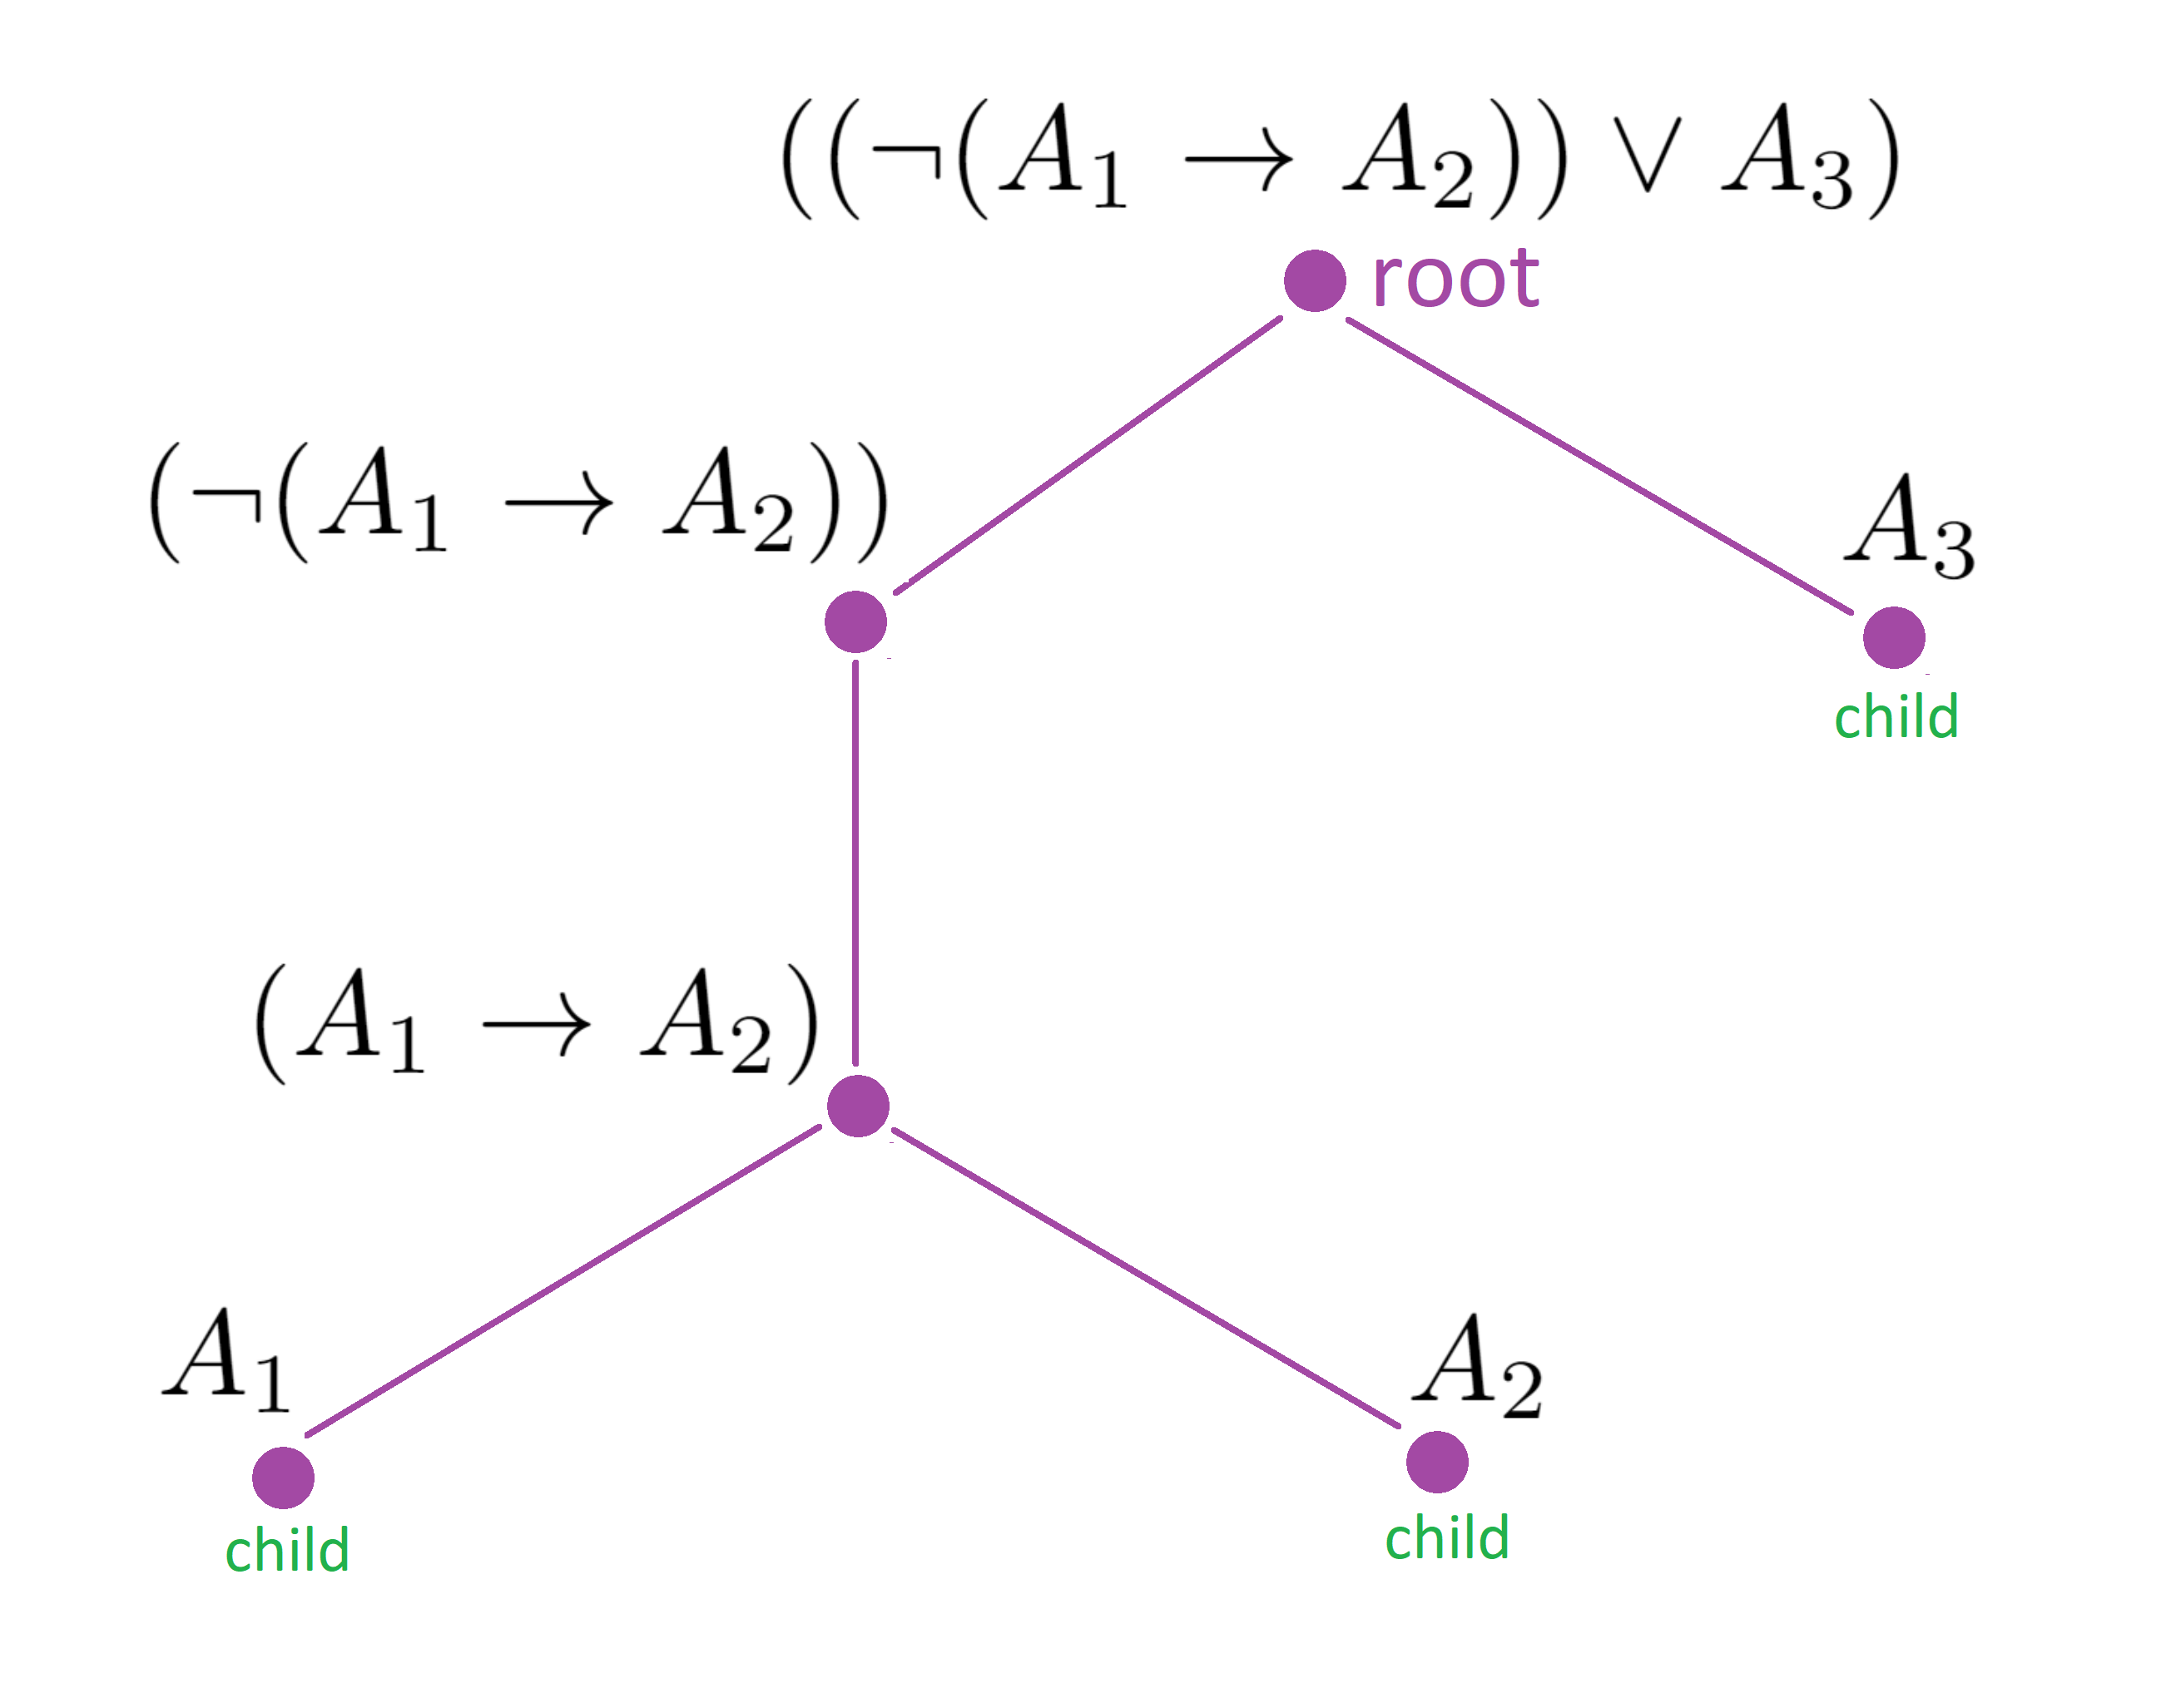
\includegraphics[width = 7cm]{1-parsing-alg-ex}
        \caption{title}
    \end{figure}
}
Back to proving the existence and uniqueness of $\overline{\nu}$ in \ref{ThrmUniqueExt}.
Let $\alpha$ be a prop. sent. of $\overline{S}$. We apply the parsing algorithm to $\alpha$ to get a unique construction tree
For the leaves, use $\nu$ go get the truth values then work our way up using the conditions (1-6) in \ref{TAConditions}.
\subsection*{A more formal notation}
TODO


\section{Induction and recursion}
\subsubsection*{Generalization of induction principle:}
Let $\mathcal{U}$ be a set and $B\subseteq \mathcal{U}$ our initial set.
$\mathcal{F} = \{f,g\}$ a class of functions containing just $f$ and $g$, where $$f:\mathcal{U}\times \mathcal{U}\to \mathcal{U}, \qquad g: \mathcal{U}\to \mathcal{U}$$
We want to construct the smallest subset $\mathcal{C}\subseteq \mathcal{U}$ such that $B\subseteq \mathcal{C}$ and $\mathcal{C}$ is closed under all elements of $\mathcal{F}$.
\defin{Closedness, Inductiveness}{ We say $\mathcal{S}\subseteq \mathcal{U}$ is 
    \begin{itemize}
        \item\graybf{closed} under $f$ and $g$ iff for all $x,y\in \mathcal{S}$ it holds $ f(x,y)\in \mathcal{S}$ and $ g(x)\in \mathcal{S}$
        \item\graybf{inductive} if $B\subseteq \mathcal{S}$ and $\mathcal{S}$ is closed under $\mathcal{F}$
    \end{itemize}
}
One way is from the top down $\mathcal{C}^* \defeq \bigcap_{\mathcal{S} \text{inductive}}{S}$
Another is from bottom up: We call $c_1 \defeq \mathcal{B}$, 
$$C_i \defeq C_{i-1} \cup \{f(x,y) : x,y\in C_{i-1}\}\cup \{g(x) : x\in C_{i-1}\}$$
and $C_* \defeq \bigcup_{n\geq 1}{C_{n}}$
Exercise: show that $C^* = C_*\eqdef C$.
Example:
\bsp{}{
    \begin{enumerate}
        \item Let $\mathcal{U}$ be the set of all expressions, $\mathcal{B}$ the set of atoms and $\mathcal{F}=\{\mathcal{E}_\square:  \square in \{\lnot, \land,\lor,\to,\leftrightarrow \}\}$
    Then $\mathcal{C}$ would be the set of all propositional formulas.
        \item Let $\mathcal{U}$ be $\RR$, $\mathcal{B}$ the set containing $0$ and $\mathcal{F}=\{S\}$, $S(x) = x+1$
        Then $\mathcal{C}$ would be the set of the natural numbers.
    \end{enumerate}
    
}
\subsubsection*{Induction principle}
$\mathcal{C}$ generated from $\mathcal{B}$ by use of elements of $\mathcal{F}$ if $S\subseteq C$ such that $\mathcal{B}\subseteq S$ and $S$ is closed under all
elements of $\mathcal{F}$, then $S = C$
proof: 
$S\subseteq C$ is clear. 
$S$ is inductive, so $C\subseteq S$.
Question: under what conditions do we get "generalized unique readability?"
The goal would be to define a function on $\mathcal{C}$ recursively i.e. to have rules for computing $\overline{h}(x)$ for $x\in B$
with some rules of computing $\overline{h}(f(x,y))$ and $\overline{h}(g(x))$ from $\overline{h}(x)$ and $\overline{h}(y)$.

\bsp{}{
    Suppose that $G$ is some additive group, generated from $\mathcal{B}$ (the set of generators), 
    $h = \mathcal{B}\to H$ where $(H,\cdot,^{-1},1)$ a group.
    When is there an extention $\overline{h}$ of $h$ s.th.
    $\overline{h}:G\to H$ is a grouphomomorphism.
    \begin{itemize}
        \item $\overline{h}(0) = 1$
        \item $\overline{h}(a+b) = \overline{h}(a)\cdot \overline{h}(b)$
        \item $\overline{h}(-a) = \overline{h}(a)^{-1}$
    \end{itemize}
    This is not always possible. \textbf{Note:} that it is possible if $G$ is generated freely by the elements of $\mathcal{B}$ and the set of atoms is independent
    (one element of $\mathcal{B}$ cannot be generated in finitly many steps by other elements of $\mathcal{B}$).
}
\defin{}{$\mathcal{C}$ is freely generated from $\mathcal{B}$ by $f,g$ if 
    \begin{itemize}
        \item $\mathcal{C}$ is generated from $\mathcal{B}$ by $f,g$ 
        \item $f|_{C^2}$ and $g|_C$ are such that\begin{itemize}
            \item $f|_{C^2}$ and $g|_C$ are one-to-one (injective)
            \item $rng(f|_{C^2})$ and $rng(g|_{C})$ and $\mathcal{B}$ are p.w. disjoint
        \end{itemize}
    \end{itemize}
}
\prop{recursion Theorem}{
    $C\subseteq U$ freely generated from $B$ by $f,g$ and $V$ a set and $h:B\to V$, $F:V^2\to V$, $G:V\to V$
    Then $\exists ! \overline{h}:\mathcal{C}\to V$ s.that 
    \begin{itemize}
        \item for all $a$ in $\mathcal{B}$ it holds $\overline{h}(a) = h(a)$
        \item for all $x,y$ in $\mathcal{C}$ it holds
        \begin{enumerate}
            \item $\overline{h}(f(x,y)) = F(\overline{h}(x),\overline{h}(y))$
            \item $\overline{h}(g(x)) = G(\overline{h}(x))$
        \end{enumerate}
    \end{itemize}
}{}
\note{}{if given conditions are satisfied then $h$ extends uniquely to a homomorphism $(C,f,g)\to (V,F,G)$}
Before we proof the recursion theorem, we will show how unique readability easily follows from it.
\note{}{Recusion Theorem implies unique readability for propositional formulas.
    What we need to check is that 
    \textbf{Claim:} The Assumptions of recursion theorem are satisfied.
    \begin{claimproof}
        {$\mathcal{F}_\lor$ is one to one, suppose $(\alpha \lor \beta) = (\delta \lor \gamma)$ then $\alpha \lor \beta) = \delta \lor \gamma)$
            And $\alpha,\delta$ are prop. formulas, so they equal to each other (else one is an initial segment of the other, hence not a prop. fla.)
            By the same argument we get $\beta$ is equal to $\gamma$.
        }
    \end{claimproof}
    \textbf{Claim: }Disjointment of ranges
\begin{claimproof}
    \begin{itemize}
        \item if $(\alpha\lor \beta)$ is $A$ then $A$ starts with $($ 
        \item if $(\alpha\lor \beta)$ is $(\gamma \to \delta)$ then by the same argument $\alpha$ is $\gamma$ but $\lor$ and $\to$ are diffrent
        \item 
    \end{itemize}

\end{claimproof}
    

}
\subsubsection*{Proof of the Rec Thm.}
$v:C\to V$ TODO partial function pfeil nur oben is called acceptable if $\forall x,y\in C$ 
\begin{enumerate}
    \item if $x\in B\cap dom(v)$ then $v(x)=h(x)$
    \item if $f(x,y)\in dom(v)$ then $x,y\in dom(v)$ and similarly for $g$
    \begin{itemize}
        \item $v(f(x,y)) = F(v(x),v(y))$
        \item $v(g(x)) = G(v(x))$
    \end{itemize}
\end{enumerate}
And when $\mathcal{U} = \{\varGamma_v : v \text{acceptable} \}$, we define
$\overline{h}\defeq \text{function w/ graph} \bigcup\mathcal{U}$

\textbf{Claim 1:} $\overline{h}$ is a function.
\begin{claimproof}
    $$S\defeq \{x\in \mathcal{C} : \exists \text{at most one $y$ w/} (x,y)\in \bigcup \mathcal{U}\}$$
    We want $S = C$, we have $S\subseteq C$,
    it is enough to show that $S$ is inductive.
    \begin{itemize}
        \item $x\in B\cap dom(v)$ for some $v$ acceptable.
        then $v(x) = h(x)$ by 1.
        also $x\notin rng f|_{C^2}$ and $x\notin rng g|_C$
        \item $x,y in \mathcal{S}$
        We want $f(x,y),g(x)\in S$
        there are $v_1,v_2$ acceptable s.t. $f(x,y)\in dom(v_1)\cap dom(v_2)$
    \end{itemize}
\end{claimproof}
\textbf{Claim 2:} $\overline{h}$ is acceptable.
\begin{claimproof}
    $\overline{h}: C \rightharpoonup V$ by definition.
    if $x\in B\cap dom \overline{h}$ then there is a $v$ acceptable, s.t. $x\in dom(v)$
    then $\overline{h}(x) = v(x)=h(x)$
    if $f(x,y)\in dom \overline{h}$ then $f(x,y)\in dom (v)$ form some $v$ acceptable.
    Hence $x,y\in dom(v)$ and therefore $x,y\in dom (\overline{h})$
    and we have $$\overline{h}(f(x,y)) = v(f(x,y)) = F(v(x),v(y)) = F(\overline{h}(x),\overline{h}(y))$$
\end{claimproof}
\textbf{Claim 3:} The domain of $\overline{h}$ equals $\mathcal{C}$. 
\begin{claimproof}
    it is enough to show that the domain of $\overline{h}$ is inductive. 
    $B\subseteq dom (\overline{h})$ bc. $B\subseteq dom (h)$ where $h$ is acceptable.
    Now we need to show closure under $f,g$. suppose $x',y'\in dom (\overline{h})$ then $x'\in dom (v_1)$ 
    for some acceptable $v_i$ lets assume $f(x',y')\notin dom (\overline{h})$
    then we extend $\overline{h}$ to a function with the same graph as $\overline{h}$.
    Then
    $\varGamma \cup \{(f(x',y'),F(\overline{x'},\overline{y'}))\}$ 
    is the graph of an acceptable function.
\end{claimproof}
\textbf{Claim 4:} Suppose both $\overline{h},\overline{\overline{h}}$ work, we schow that $S=\{x\in C: \overline{h}(x),\overline{\overline{h}}(x)\}$ is the whole set $C$.
it is enough to show that $S$ is inductive.

Let $x\in B$ then $\overline{h}(x) = h(x) = \overline{\overline{h}}(x)$.
Then for $x,y\in S$ \[\overline{h}(f(x,y)) = F(\overline{h}(x),\overline{h}(y))=  F(\overline{\overline{h}}(x),\overline{\overline{h}}(y))=\overline{\overline{h}}\dots \]
\section{Sentential connectives}
\defin{Tautological equivalence relation}{For $\alpha,\beta$ prop. sent. we define $\alpha \sim \beta$ 
iff $\alpha \sledom\models  \beta$. This defines an equivalent relation.}
\bsp{}{$A \to B \sledom\models  \lnot A \lor B$}
\note{}{
    A $k$-place boolean function is a functon of the form $f: \{0,1\}^k\to \{0,1\}$ and we 
    define $0,1$ as the $0$-place boolean functions.\\
    If $\alpha$ is a prop. sent. then it determines a $k$-place boolean function, 
    where $k$ is the number of atoms, $\alpha$ is built up from.
    If $\alpha$ is $A_1\lor \lnot A_2$ then $B_\alpha: \{0,1\}^2\to \{0,1\}$ and asign its values corresponding a truth table.
    TODO extend / rearange function
}
\prop{}{If $\alpha,\beta$ are prop. sent. with at most $n$ prop. Atoms (combined), then
    \begin{enumerate}
        \item $\alpha \models \beta $ iff $\forall x\in \{0,1\}^n$ it holds $B_\alpha(x)\leq B_\beta(x)$
        \item $\alpha \sledom \models \beta $ iff $\forall x\in \{0,1\}^n$ it holds $B_\alpha(x) = B_\beta(x)$
        \item $\models \alpha $ iff $\forall x\in \{0,1\}^n$ it holds $B_\alpha(x)=1$
    \end{enumerate}
}{}
\prop{Realisation}{
    Let $G$ be an $n$-ary boolean function for $n\geq 1$. Then there is a prop. sent. $\alpha$ such that. $B_\alpha = G$.
    We say $\alpha$ realizes $G$.
}{
    \begin{enumerate}
        \item if $G$ is constantly equal to $0$ then set $\alpha$ to $A_1 \land \lnot A_1$.
        \item Otherwise the set of inputs $\{\vec{x}_1,\vec{x}_2,\dots \vec{x}_k\}$ for which $G(\vec{x}_i)=1$ holds is not empty.\\
        We denote $\vec{x}_i = (x_{i1},x_{i2},\dots x_{in})$ and define a matrix $(x_{ij})_{k\times n}$
        We further set $\beta_{ij} = \begin{cases}
            A_j & \text{iff } x_{ij}=1\\
            \lnot A_j & \text{iff } x_{ij}=0
        \end{cases}$\\
        \graybf{Example:} 
        \begin{equation*}
            (x_{ij})=
            \begin{pmatrix}
                0&1&0\\
                1&1&0
            \end{pmatrix}\leadsto 
            \begin{pmatrix}
                \lnot A_1 & A_2 & \lnot A_3\\
                A_1 & A_2 & \lnot A_3\\
            \end{pmatrix}=(\beta_{ij})
        \end{equation*}
        We define $\gamma_i$ as $\beta_{i1} \land \beta_{i2}\land \dots \beta_{in}$ for $1\leq i\leq k$\\
    and $\alpha$ as $\gamma_1 \lor \gamma_2\lor \dots \gamma_k = \vee_{i=1}^{k}{\gamma_i} $
    Then $B_\alpha = G$ is fulfilled.
    \end{enumerate}
}
\note{}{$\alpha$ as constructed in the proof is in the so-called Disjunctive normal form (DNF).}
\coroll{Every prop. sent. is tautologically equivalent to a sentence in DNF}
\addAbbrev{i.e.}{id est (that is)}
\coroll{$\{\lnot,\land,\lor\}$ is a complete set of logical connectives, i.e. every prop. sent. is tautologically 
    equivalent to a sentence built up from atoms and $\lnot,\land,\lor$.
}
\prop{}{Both $\{\lnot, \land\}$ and $\{\lnot, \lor\}$ are complete.}{
    Its sufficient to show that every $k$-place boolean function is realisable by a prop. sent.
    built up using only $\lnot$ and $\land$. This is, because $\alpha\land \beta \sledom \models \lnot (\lnot \alpha \lor \lnot \beta)$
    We prove this by induction over the number of disjuctions of a prop. sent. $\alpha$ in DNF.
    Suppose the statement is true for $k \leq n$. For $n+1$ and $\alpha = \bigvee_{j=1}^{n+1}{\gamma_j}$ there exists an $\alpha' \sledom \models \bigvee_{j=1}^{n}{\gamma_j}$ and 
    $$\alpha = \bigvee_{j=1}^{n+1}{\gamma_j} \sledom \models \alpha' \lor \gamma_{n+1} \sledom \models \lnot (\lnot \alpha' \land \lnot \gamma_{n+1})$$
    %$\alpha\land \beta \sledom \models \lnot (\lnot \alpha \lor \lnot \beta)$
}
\note{}{We used the observation that, if $\alpha \sledom \models \beta$ and we replace a subsequence of $\alpha$ by a so called tautological equivalence 
    then the result is also tautologically equivalent to $\beta$}
TODO S.10
\bsp{$\{\to, \land\}$ is not complete.}{Let $\alpha\in PS$ built up from only $\to,\land$ from the atoms $A_1,\dots A_n$ then we claim
    $$A_1\land A_2\land \dots \land A_n \models \alpha$$
    %Furhter we can observe that $\{\to, \lor \}$ is not complete, because if $\alpha\in PS$ is only built up from $\to,\lor$ then $\lnot \alpha$
    %can be built up from $\to, \land$. This is because of
    %$$\lnot(A\to B)\sledom \models \lnot B \to \lnot A \quad \text{and}\quad \lnot(\alpha\lor \beta) \sledom \models \lnot \alpha \land \lnot \beta$$
    We can also say $\{\to, \land\}$ is not complete bc. $\lnot A$ is not tautological equivalent to a sent. built up from $\to, \land$
    \begin{proof}
        Let $C \defeq \{\alpha \in PS \text{ built up from }\to,\land \text{ and }A_1,\dots A_n \text{ for which } \bigwedge_{i=1}^n{A_i}\models \alpha\}$
        we want to show that $C = \{\alpha \in PS \text{ built up from }\to,\land \text{ and }A_1,\dots A_n \}$
        \begin{itemize}
            \item We have $\{A_1,A_2\dots,A_n\}\subseteq C$
            \item for $\alpha,\beta\in C$ it holds
            \begin{itemize}
                \item[(1)] $A_1\land\dots\land A_n \models \alpha\to\beta$
                \item[(2)] $A_1\land\dots\land A_n \models \alpha\land \beta$
            \end{itemize}
        \end{itemize}
        Therefore $C$ is closed under the fla. building operations and we have proven our claim.
    \end{proof}
    }
\note{}{$\{\land,\lor,\to,\leftrightarrow \}$ is still not complete.}
\note{}{The number of $n$-ary boolean functions existing is $2^{2^n}$
    We define a notation for $n=0$: $\bot$ (for TV = $0$) and $\top$ (for TV = $1$)
    We can conclude that $\{\lnot,\to\}$ and $\{\to, \bot\}$ are both complete, it holds $\lnot A \sledom \models A\to \bot$
}
\defin{Satisfiability}{\\ A set of prop. sent. $\Sigma$ is called \graybf{satisfiable} iff $\exists$ TA that satisfies every member of $\Sigma$.}
\section{Compactness Theorem}
\prop{Compactness Theorem}{\label{CompThrm}
    $\Sigma$ is satisfiable iff every finite subset $\Sigma_0\subseteq \Sigma$ is satisfiable. (i.e. $\Sigma$ is finitely satisfied)}{
    Let $\Sigma$ be a finitely satisfiable set of prop. sent. Outline of the proof:
    \begin{enumerate}
        \item extend $\Sigma$ to a maximal finitely satisfiable set $\Delta$ of prop. sent.
        \item construct a thruth assigment using $\Delta$
    \end{enumerate}
    \begin{enumerate}
        \item Let $\alpha_1,\alpha_2,\dots$ be an enumeration of all prop. sent. 
        and define $\Delta_n$ inductively by $\Delta_0 \defeq \Sigma$
        $$\Delta_{n+1}\defeq \begin{cases}
            \Delta_n\cup \{\alpha_{n+1}\} & \text{if satisfiable}\\
            \Delta_n\cup \{\lnot\alpha_{n+1}\} & \text{otherwise}
        \end{cases}$$
        \textbf{Claim:} $\Delta_n$ is finitely satisfiable for each $n$
        \begin{claimproof}
            By regular induction over $n$. $\Delta_0$ is finitely satisfiable. Let us assume $\Delta_n$ is finitely satisfiable.
            If $\Delta_{n+1} = \Delta_n\cup \{\alpha_{n+1}\}$ then we are finished. 
            Otherwise let $\Delta' \subseteq \Delta_n$ be a finite set that $\Delta' \cup \{\alpha_{n+1}\}$ is not satisfiable.
            It holds $\Delta' \models \lnot \alpha_{n+1}$.
            We assume that $\Delta_n\cup \{\lnot\alpha_{n+1}\}$ is not finitely satisfiable. 
            Then there exists a finite subset $\Delta'' \subseteq \Delta_n $ such that $\Delta'' \cup \{\lnot\alpha_{n+1}\}$ is (finite and) not satisfiable.
            It therefore holds $\Delta'' \models \alpha_{n+1}$
            But $\Delta'\cup \Delta''$ is a finite subset of $\Delta_n$ and by above observations $\Delta'\cup \Delta''\models \alpha_{n+1}$ and $\Delta'\cup \Delta''\models \lnot \alpha_{n+1}$
            A contradiction to the assumption that $\Delta_n$ is finitely satisfiable.
        \end{claimproof}
        We set $\Delta \defeq \bigcup_{i\in\NN}{\Delta_i}$ and get
        \begin{enumerate}
            \item $\Sigma\subseteq \Delta$
            \item (Maximality): for every prop. sent. $\alpha$ it holds $\alpha\in \Delta$ or $\lnot \alpha\in \Delta$
            \item (Satisfiability): $\Delta$ is finitely satisfiable. For every finite subset there exists a $\Delta_n$ which is a superset.
        \end{enumerate}
        \item Let $\nu$ be a TA for the prop. atoms $A_1, A_2,\dots$ such that $\nu(A) = 1$ iff $A\in \Delta$
        
        \textbf{Claim:} For every prop. sent. $\varphi$ it holds $\overline{\nu}(\varphi) =1 $ iff $\varphi\in\Delta$.
        \begin{claimproof}
            Let $S = \{\varphi \in PS \text{ s.t. } \overline{\nu}(\varphi) = 1 \text{ iff } \varphi \in \Delta\}$. \\
            \begin{itemize}
                \item $PS\supseteq S$ is clear.
                \item $PS\subseteq S$ 
                \begin{enumerate}
                    \item $\{A_1,A_2\dots\}\subseteq S$ by definition of $\nu$
                    \item closure under $\epsilon_\lnot$: Let $\varphi\in S$ then we get by maximality and satisfiability of $\Delta$: 
                    \begin{equation*}
                        \begin{split}
                            &\overline{\nu}(\lnot\varphi) = 1\\
                            \text{iff }\quad&\overline{\nu}(\varphi) = 0\\
                            \text{iff }\quad& \varphi \notin \Delta\\
                            \text{iff }\quad& (\lnot \varphi)\in \Delta
                        \end{split}
                    \end{equation*}
                    closure under $\epsilon_\to$: Let $\varphi_1,\varphi_2\in S$ similiarly
                    \begin{equation*}
                        \begin{split}
                            &\overline{\nu}(\varphi_1\to \varphi_2) = 0\\
                            \text{iff }\quad&\overline{\nu}(\varphi_1) = 1 \text{ and } \overline{\nu}(\varphi_2) = 0\\
                            \text{iff }\quad& \varphi_1 \in \Delta \text{ and }\varphi_2 \notin \Delta\\
                            \text{iff }\quad& (\varphi_1\to \varphi_2)\notin \Delta 
                        \end{split}
                    \end{equation*}
                    The closure under the other fla. building operations are similar.\qedhere
                \end{enumerate}
            \end{itemize}
        \end{claimproof}
        By this claim $\overline{\nu}$ satisfies $\Sigma$.\qedhere
    \end{enumerate}
}
\coroll{\label{CorCompThrm}
    If $\Sigma\models \tau$ then there exists a finite subset $\Sigma' \subseteq \Sigma$ s.t. $\Sigma' \models \tau$}
\begin{proof}
    Recall: $\Sigma\models \tau$ iff $\Sigma\cup\{\lnot \tau\}$ is not satisfiable.
    Suppose $\Sigma\models \tau$ but no finite subset does. \\
    Then $\forall \Sigma'\subseteq \Sigma \text{ finite } \Sigma'\cup \{\lnot \tau\}$ is satisfiable.
    By the compactness theorem $\Sigma\cup \{\lnot \tau\}$ is satisfiable which is a contradiction to $\Sigma\models \tau$.
\end{proof}
\note{}{\ref{CompThrm} and \ref{CorCompThrm} are equivalent.}


\chapter{Predicate - / first order logic}
The definitions, lemmata, propositions and theorems as well as the notes in this chapter are sourced from \cite[chapter~2]{EndertonHerbertB2001AMIt}.
\defin{A First order Language}{
    consists of infinetely many distinct symbols such that no symbol is a proper 
    initial segment of another symbol. The symbols are divided into 2 groups:
    \begin{enumerate}
        \item logical symbols\outernote{logical symbols}\\
        (These elements have a fixed meaning and the equivalence symbol $=$ is optional)
        \begin{flalign*}
            (,\:),\: \lnot,\:  \to,\:  v_1,\: v_2,\: \dots,\: =&&
        \end{flalign*}
        \item parameters\outernote{parameters}
        \begin{enumerate}
            \item quantifier symbol: $\forall$ (the range is subject of interpretation)
            \item predicate symbols: for every $n>0$ we have a set of $n$-ary predicates $P$
            \item constant symbols: Some set of constants
            \item function symbols: for every $n>0$ we have a set of $n$-ary function symbols
        \end{enumerate}
    \end{enumerate}
}
\note{}{
    \begin{itemize}
        \item The sets in Group 2, (b)-(d) can also be the empty set
        \item We could drop constants and instead introduce $0$-ary function symbols
        \item to specify language we need to specify the parameters and say if $=$ is included
        \item In the book \cite{EndertonHerbertB2001AMIt} they assume that
        some $n$-place predicate symbol is present for some $n$.
    \end{itemize}
}
\bsp{}{
    \begin{itemize}
        \item $\mathcal{L}_\text{set} = \{\in\}$, \quad $=$ included and the binary predicate symbol $\in$ "element in"
        \item $\mathcal{L}_\text{arith} = \{<,0,S,E,+,\cdot\}$
        \begin{itemize}
            \item [$=$] included
            \item [$<$] is a binary rel. symbol
            \item [$0$] is a constant
            \item [$S$] is a unary function symbol
            \item [$E$] is a unary function symbol (exponentiation)
            \item [$+,\cdot$] are binary function symbols
        \end{itemize}
        \item $\mathcal{L}_\text{ring} = \{=,+,\cdot,-,0,1\}$
        \begin{itemize}
            \item [$=$] included
            \item [$0,1$] are constants
            \item [$-$] is a unary function symbol (additive inverse)
            \item [$+,\cdot$] binary function symbols
        \end{itemize}
    \end{itemize}
}

\section{Formulas}
\defin{Expression}{An \imp{expression} is any finite sequence of symbols.
    There exist two kinds of expressions that make sense ``grammatically'' The intuition should be:
    \begin{itemize}[leftmargin=1.6cm]
        \item[Terms:] \begin{itemize}
            \item points to an object
            \item they are built up from variables and constants using function symbols %(by use of polish notation)
        \end{itemize}
        \item[Formulas:]\begin{itemize}
            \item They express assertions about objects,
            \item they are built up from atomic formulas 
            \item atomic formulas these are built up from terms using predicate symbols and $=$, if included
        \end{itemize}
    \end{itemize}
}
\defin{Term Building Operations}{
    For every $n>0$ and for every $n$-place function symbol $f$, let $\mathcal{F}_f$ be an $n$-place term building operation,
    that is $\mathcal{F}_f (t_1,\dots t_n)\defeq ft_1\dots t_n$ (polish notation for $f(t_1,\dots t_n)$).
    \imp{Term}, the set of terms is defined as the set of expressions that are built up from variables and constants by applying the term building operations
    finitely many times.
}
\bsp{}{Let $\mathcal{L} = \mathcal{L}_{arith}$, the set of terms will contain $0$, $v_{42}$, $S0$, $SSS0$, $Sv_1$, $+SOv_1$}
\defin{Atomic formula}{Any expression of the form 
    $$=t_1t_2 \text{ or } Pt_1,\dots t_n, \text{ where $t_1,\dots t_n$ are terms and $P$ is an $n$-ary predicate symbol}$$
    is called \imp{atomic formula}.}
\note{}{Atomic formulas are not defined inductively.}
\bsp{}{\emph{cont.}\quad $=v_1 v_{42}$ and $<S0 SS0$ are atomic formulas, but $\lnot = v_1 v_{42}$ is not.}
\defin{Formulas}{We define $\varepsilon_\lnot$, $\varepsilon_\to, Q_i$ to be the fla. building operations, defined as follows
    $\varepsilon_\lnot(\alpha) \defeq (\lnot \alpha)$, $\varepsilon_\to \defeq (\alpha \to \beta)$ and
    $Q_i(\gamma) \defeq \forall v_i \gamma$.
    The set of formulas\outernote{formula}is the set of expressions built up from atomic formulas by applying the fla. building operations finitely many times.
}
\bsp{}{\emph{cont.} $\forall v_1 (=Sv_10)$ is a formula we get by applying $Q_1$ on the atomic formula $=Sv_1 0$.}
\subsubsection*{Free variables}
\bsp{}{We introduce the \imp{$\exists$ quantifier} as an abbreviation: $\exists y \alpha$ means $\lnot \forall y \lnot \alpha$.\\
    "Every non-zero natual number is a succsesor" $\forall x (x\neq 0\to \exists y S(y)=x)$
    is different then "if a number is not $0$, then it is a succsesor" $x\neq 0\to \exists y S(y)=x$. 
    We say, $x$ occurs \textbf{bounded}\outernote{bounded variable}in the first formula, for the latter $x$ occures free in the formula.
    If you have an expression without free variables, it is either true or false, on the other hand
    if a variable occurs free in a formula, the truth value of it depends on the variable itself.
}
\defin{Free variables}{
    Let $x$ be a variable. We say ``$x$ occurs \graybf{free in $\varphi$}'', if
    \begin{enumerate}
        \item If $\varphi$ is an atomic fla. then $x$ occurs \graybf{free} in $\varphi$ iff $x$ occurs in $\varphi$
        \item If $\varphi \equiv (\lnot \alpha)$ then $x$ occurs free in $\varphi$ iff $x$ occurs free in $\alpha$
        \item If $\varphi \equiv (\alpha \to \beta)$ then $x$ occurs free in $\varphi$ iff $x$ occurs free in $\alpha$ or $\beta$
        \item If $\varphi \equiv \forall v_i \alpha$ then $x$ occurs free in $\varphi$ iff $x$ occurs free in $\alpha$ and $x\lnot v_i$
    \end{enumerate}
    A formula $\alpha$ is called a \imp{sentence}, if no variable occurs free in $\alpha$
}
\note{}{The above definition is well defined thanks to the recursion theorem.\\
    To prove this, define the function $h$ on the set of atoms: $h(\alpha) = \{v\in V : v\text{ occurs free in }\alpha\}$, which is the set of all variables $v_i$ that occur free in $\alpha$.
    we now want to extend $h$ to $\overline{h}$ on the set of all formulas. We observe
    \begin{itemize}
        \item $\overline{h}(\lnot \alpha) = \overline{h}(\alpha)$
        \item $\overline{h}( \alpha \to \beta) = \overline{h}(\alpha)\cup \overline{h}(\beta)$
        \item $\overline{h}(Q_i(\alpha)) = \overline{h}(\alpha)\backslash \{v_i\}$
    \end{itemize}
    Then $x$ occurs free in $\alpha$ iff $x\in \overline{h}(\alpha)$.
}
\note{}{From now on, we will now use $\neq, \land,\lor, \leftrightarrow, \exists v_i$ as abbreviations in our formulas (all can be expressed in terms of $\lnot,\to,\forall_i$), so there is no ambiguity on the in the sense of the meaning of the formulas.
    Note: We will sometimes drop the $(,)$ and not always be using polish notation.
}
\section{Semantics of first order logic}
The equivalent scheme to our TA in predicate logic. The meaning of formulas is given by \imp{structures}, 
which also determine the scope of the quantifier $\forall$, the meaning of all parameters.
\defin{structure}{A \imp{structure} $\mathcal{A}$ for a first order language $\mathcal{L}$ is a non-empty set
    set $A$ called \graybf{universe} or \graybf{underlying set of $\mathcal{A}$} together with an interpretation of each parameters of $\mathcal{L}$ i.e.
    \begin{itemize}
        \item $\forall$ ranges over the universe $A$
        \item for an $n$-ary pred. symbol $P\in \mathcal{L}$ its interpretation $P^\mathcal{A}$ is a subset of $A^n$\outernote{interpretation}
        \item for a constant $c\in \mathcal{L}$ its interpretation $c^\mathcal{A}$ is an element of $A$
        \item for an $n$-ary function symbol $f\in \mathcal{L}$ its interpretation $f^\mathcal{A}$ is a total function $$f^\mathcal{A}: A^n \to A$$
    \end{itemize}
}
\note{}{$A\neq \varnothing$, and all functions $f^\mathcal{A}$ are total.}
\bsp{}{Let $\mathcal{L} = \{\in\}$ where $\in$ is a binary relation "
    An example of an $\mathcal{L}$ structure is $(\NN, \in^\NN)$ where $\in^\NN = \{(x,y)\in \NN^2 : x<y\}$}
\defin{Assigment}{Let $\varphi$ be a $\mathcal{L}$-fla. and $\mathcal{A}$ a $\mathcal{L}$-structure. 
    Let $V$ be the set of all variables in $\mathcal{L}$. Any function $s:V\to A$ is called assignment.\outernote{assigment}
    We define the extention $\overline{s}$ of $s$ to the set of all $\mathcal{L}$-terms by
    \begin{itemize}
        \item if $x\in V$ then $\overline{s}(x) \defeq s(x)$
        \item if $c\in \mathcal{L}$ is a constant symbol, then $\overline{s}(c) \defeq c^\mathcal{A}$
        \item for $t_1,\dots t_n$ $\mathcal{L}$-terms and $f\in \mathcal{L}$ an $n$-ary function symbol, 
        $$\overline{s}(ft_1\dots t_n) \defeq f^\mathcal{A}(\overline{s}(t_1),\dots \overline{s}(t_n))$$
    \end{itemize}
}

\note{}{in the previous definition point 3. for $n=1$ yields a commutative diagram.

}
\thm{}{For any given assignment $s$ there exists a unique extention $\overline{s}$ as in the previous definition.}
{
    will follow from recursion theorem and unique decomposition of terms.
}
\newpage
\subsection*{Satisfaction and Models}
\defin{Satisfy}{ We define '$\mathcal{A}$ satisfies $\varphi$ with $s$' and write
    $\mathcal{A}\models \varphi \:[s]$\outernote{$\models_\mathcal{A}$}\\
    or $\models_\mathcal{A} \varphi \:[s]$, if (inductively over the complexity of the formula $\varphi$)
    \begin{enumerate}
        \item if $\varphi$ is atomic: \begin{itemize}
            \item $\mathcal{A} \models\: = t_1,t_2 \: [s]$ iff $ \overline{s}(t_1) = \overline{s}(t_2)$
            \item $\mathcal{A} \models P t_1,\dots t_n \: [s]$ iff $(\overline{s}(t_1),\dots \overline{s}(t_2))\in P^\mathcal{A}$
        \end{itemize}
        \item suppose $\mathcal{A}\models \varphi \: [s]$ and $\mathcal{A}\models \psi \: [s]$ are defined, then
        \begin{itemize}
            \item $\mathcal{A}\models \lnot\varphi \: [s]$ iff $\mathcal{A}\not\models \varphi \: [s]$
            \item $\mathcal{A}\models \varphi\to \psi \: [s]$ iff $\mathcal{A}\models \psi \: [s]$ or $\mathcal{A}\not\models  \varphi \: [s]$
            \item $\mathcal{A}\models \forall x \varphi \: [s]$ iff for all $a\in A$ $\mathcal{A}\models \varphi [s(x| a)]$
            where 
            \begin{equation*}
                s(x|a)(v) \defeq \begin{cases}
                s(v) \text{ if } v \neq x\\
                a \text{ if } v = x
            \end{cases}
            \end{equation*}
            
        \end{itemize}
    \end{enumerate}
}
\bsp{}{
    $\mathcal{L} = \{\forall, \leq, S, 0\}$ 
    an example of an $\mathcal{L}$-structure $\mathcal{N} = (\NN,\leq^\mathcal{N},S^\mathcal{N},0^\mathcal{N})$. Together with a specified assignment
    $s: v_n \mapsto n-1$ 
    \begin{itemize}
        \item $s(v_1) = 0$
        \item $\overline{s}(0) = 0^\mathcal{N}$ (a constant is always mapped to its realisation, the interpretation of constant $0$ in the structure $\mathcal{N}$)
        \item $\overline{s}(Sv_1) = S^\mathcal{N}(\overline{s}(v_1)) = S^\mathcal{N}(0) = 1$\\
        \item $\mathcal{N}\models \forall v_1 (S(v_1) \neq v_1) \: [s]$\\
            iff for all $a\in \NN$ we have that $\mathcal{N}\models (S(v_1) \neq v_1) [s(v_1 | a)]$\\
            iff \dots \\
            iff for all $a\in \NN$ we have $S^\mathcal{A}(a) \neq a$, which is true in our structure of the natural numbers.
        \item Is it true in $\mathcal{N}$ that $\mathcal{N}\models S(0) \leq S(v_1) \: [s]$? Yes because
        \begin{equation*}
            \begin{split}
                &\mathcal{N}\models S(0) \leq S(v_1) \: [s] \\
                &\iif \: 1\leq 1
            \end{split}
        \end{equation*}
        
    \end{itemize}
}

To know wheter $\mathcal{A}\models \varphi \: [s]$ it suffices to know where $s$ maps the variables that occur free in $\varphi$. This results from the Coincidence Lemma \ref{Thm.evalonlyfreevar}
\thm{Coincidence Lemma}{\label{Thm.evalonlyfreevar}Suppose $s_1,s_2:V\to A$ agree on all variables that occur free in $\varphi$ then 
 $$\mathcal{A}\models \varphi \:[s_1] \text{ iff }\mathcal{A}\models \varphi \: [s_2]$$
}{
    By complexity of $\varphi$
    \begin{enumerate}
        \item if $\varphi$ is $P t_1,\dots t_n$ 
        note: any var that occur in $\varphi$ occur free in $\varphi$, so $s_1,s_2$ agree on all variables that occur in the terms $t_1,\dots t_n$.\\
        So we Claim: for $t$ a term, $s_1,s_2$ assignments that agree on all variables of $t$ then $\overline{s}_1(t) = \overline{s}_2(t)$
        \begin{claimproof}
            By complexity of $t$
            \begin{itemize}
                \item $t = v_m$ then  $\overline{s}_1(t) ={s}_1(v_m) = {s}_2(v_m) =\overline{s}_2(t)$
                \item $t = c$ then  $\overline{s}_1(t) =c^\mathcal{A} =\overline{s}_2(t)$
                \item $t = ft_1\dots t_n$ inductively, assume $\overline{s}_1(t_i) =\overline{s}_2(t_i)$ for all $1\leq i\leq n$ then  TODO
            \end{itemize}
        \end{claimproof}
        \item if $\varphi$ is $ =t_1,t_2$ is similar
        \item if $\varphi$ is $\lnot \alpha$ then $\mathcal{A}\models \lnot \alpha  \: [s_1]$ iff $\mathcal{A}\not\models \alpha  \: [s_1]$ iff $\mathcal{A}\not\models \alpha  \: [s_2]$ iff $\mathcal{A}\models \lnot \alpha  \: [s_1]$
        \item if $\varphi$ is $\alpha \to \beta$ then $\mathcal{A}\models  \alpha \to \beta  \: [s_1]$ iff .. or .. iff for s2 iff ... or .. 
        \item if $\varphi$ is $ \forall x \alpha$ then the assumption is that $s_1,s_2$ .. the free variables of $\alpha$ are the free variables of $\varphi$ exept for $x$.
        but because $s_1(x|a) = s_2(x|a)$ they both agree on all free variables of $\alpha$.
        \[\begin{split}
            \mathcal{A}\models \forall x \varphi  \: [s_1] &\iif \fora a\in A \mathcal{A}\models \varphi  \: [s_1(x| a)]\\
            & \iif \fora a\in A \mathcal{A}\models \varphi  \: [s_2(x| a)]\\
            & \iif \mathcal{A}\models \forall x \varphi  \: [s_2]
        \end{split}\]
    \end{enumerate}
    
}
Notation: if all free variables of $\varphi$ are among $v_1,\dots v_n$ and the assigment $s(v_i) = a_i$ for all $1\leq i\leq n$ we write 
$$\mathcal{A}\models \varphi \llbracket a_1,a_2,\dots, a_n\rrbracket\defeq \mathcal{A}\models \varphi \: [s]$$
\note{}{If $\sigma$ is a sentence then we can not have $\mathcal{A}\models \sigma$ and $\mathcal{A}\not\models \sigma$ because $A\neq \varnothing$.}
\coroll{If $\sigma$ is a sentence then either $\mathcal{A}\models \sigma \: [s]$ for all $s:V\to A$ or 
$\mathcal{A}\not\models \sigma \: [s]$ for all $s:V\to A$.
}
\noindent Notation: $\mathcal{A}\models \sigma$ and we say ``$\sigma$ is true in $\mathcal{A}$'' or ``$\mathcal{A}$ is a model of $\sigma$'' or ``$\sigma$ holds in $\mathcal{A}$''.

\defin{Model}{$\mathcal{A}$ is sayed to be ``a model of a set of sentences $\Sigma$'' $\mathcal{A}\models \Sigma$, if for every sentence $\sigma\in \Sigma$ it holds $\mathcal{A}\models \sigma$ }
\bsp{}{$\mathcal{L} = \{0,1,+,-,\cdot\}$
A Structure could be $\mathcal{R} = (\RR, 0,1,+,-,\cdot)$ or $\mathcal{C} = (\mathbb{C}, 0,1,+,-,\cdot)$
then the sentence 
$\sigma: \quad \exists x (x\cdot x = -1)$ then $\mathcal{R}\not\models \sigma$ but $\mathcal{C}\models \sigma$
}
\note{}{$\land,\lor,\leftrightarrow,\exists$ work as expected. That is 
 $\mathcal{A}\models (\alpha \land \beta) \: [s]$ iff $\mathcal{A}\models \alpha \: [s]$ and $\mathcal{A}\models \beta \: [s]$
 $\mathcal{A}\models (\alpha \lor \beta) \: [s]$ iff $\mathcal{A}\models \alpha \: [s]$ or $\mathcal{A}\models \beta \: [s]$
 $\mathcal{A}\models \exists x \alpha \: [s]$ iff $\mathcal{A}\models \lnot \forall x \lnot \alpha \: [s]$\\
 iff $\mathcal{A}\not\models \forall x \lnot \alpha \: [s]$\\
 iff it is not true that forall $a \in A$ $\mathcal{A}\models \lnot \alpha [s(x|a)]$\\
 iff there is $a\in A$ such that $\mathcal{A}\models \alpha [s(x|a)]$
}

\subsection*{Logical implication}
Let $\Gamma$ be a set of $\mathcal{L}$-formulas, $\varphi$ a $\mathcal{L}$-formula.
\defin{Logical implication}{
    We say ``$\Gamma$ logically implies $\varphi$'' $\Gamma \models \varphi$, if\\
    for every $L$-structure $\mathcal{A}$ and for every assigment $s:V\to A$ 
    $$\text{if } \mathcal{A}\models \gamma [s]\text{ for every $\gamma\in \Gamma$, then }\mathcal{A}\models \varphi \: [s]$$
}

\defin{Logical equivalence}{Two formulas $\varphi,\psi$ are called logically equivalent, if 
$\varphi \models \psi$ and $\psi \models \varphi$.
}
\defin{Valid}{A formula $\varphi$ is called valid, if $\models \varphi$ i.e. $\varnothing\models \varphi$ i.e. for every $\mathcal{L}$-structure $\mathcal{A}$ and every $s:V\to A$ it is $\mathcal{A}\models \varphi \: [s]$
}
\bsp{}{
\begin{enumerate}
    \item $\forall x_1 P x_1 \models P x_2$\\
    Suppose $\mathcal{A}\models \forall x_1 P x_1 \: [s]$.
    then for all $a\in A$ it is $\mathcal{A}\models P x_1 [s(x_1|a)]$ in particular, $a\in P^\mathcal{A}$ for $a = s(x_2)$
    \item  $\forall P x_2 \not\models \forall x_1 P x_1$\\
    We need a counterexample to $\forall P x_2 \models \forall x_1 P x_1$. Let $A = \{a_1,a_2\}$ $s(x_2) = a_1$ and $P^\mathcal{A} = \{a_1\}$
    then $\mathcal{A}\models Px_2 \: [s]$.
    \item Is the following valid? $\models \exists x(Px \to \forall y P y)$ yes
    \item $\Gamma,\alpha\models \varphi$ iff $\Gamma \models \alpha \to \varphi$. (on next problem set, quite important)
\end{enumerate}
}

\section{definability in a structure}
By choosing a language $\mathcal{L}$, we specify which constant, function and relation symbols we can use when constructing formulas. If we then fix a structure $\mathcal{A}$, some $n$-ary relations that may are not in our structure, can still be expressed by a formula $\varphi$. For example given the structure $\mathcal{N} = (\NN;0,+)$ with equality and the usual addition on $\NN$, we can view the set
\[P_< \defeq \{(n,m)\in \NN : \varphi(n,m)\},\quad \varphi(n,m)\equiv \exists x \, (\lnot(x=0)\land n+x=m)\]
That gives us the usual interpretation of $<$ in the natural numbers, namely $n<m$ iff $\varphi(n,m)$ iff $(n,m)\in P_<$. 
\defin{definability in a structure}{ 
    We say that a general $n$-ary relation $P$ on $A$ (we will just call it $P$, it does not have to be in the language) is definable in $\mathcal{A}$, if there is a $\mathcal{L}$-formula
    $\varphi$ with free variables among $\{v_1,\dots,v_n\}$ such that 
    \[P = \{(a_1,\dots a_n) \in A^n: \mathcal{A} \models \varphi\: \llbracket a_1,\dots a_n\rrbracket\}\]
    We also say that $\varphi$ defines $P$ in the structure $\mathcal{A}$.
    
    TODO definability by points:\outernote{definable by points}
    We say that a general $n$-ary relation $P$ on $A$ is definable \graybf{by points} in $\mathcal{A}$, if there is a $\mathcal{L}$-formula
    $\varphi$ with free variables among $\{v_1,\dots,v_{n+m}\}$ and $b_1,\dots b_m\in A$ such that 
    \[P = \{(a_1,\dots a_n) \in A^n: \mathcal{A} \models \varphi\: \llbracket a_1,\dots a_n, b_1,\dots b_m\rrbracket\}\]
}
\bsp{}{
    \begin{enumerate}
        \item $x = x$ would define the entire universe.
        \item $\lnot x = x$ would define the empty set.
    \end{enumerate}
}
\bsp{}{
\begin{enumerate}
    \item TODO
    \item $\mathcal{R} = (\RR,0,1,+,-,\cdot)$ Q: is $[0,\infty)$ definable in $\mathcal{R}$
    Yes because $\exists y (y\cdot y = x)$
    Indeed we can even define the $\leq$ relation on $\RR^2$ by $x\leq z \defaq \exists y (x+y\cdot y = z)$ 
\end{enumerate}
}
\defin{definability of classes of structures}{
    Let $\Sigma$ be a set of sentences. $\tau$ a sentence.
    The class of models of $\Sigma$ is the class $\Mod \Sigma =\{\mathcal{A} : \mathcal{A}\models \Sigma\}$.
    Let $K$ be a class of structures. We are going to call $K$ an elementary class (EC) if there is a single sentence $\tau$ such that $K = \Mod \tau$.
    $K$ is called an elementary class in the wider sence (EC$_\Delta$) if there is a set of sentences $\Sigma$ such that $K = \Mod \Sigma$

}
\bsp{}{Let $\mathcal{L} = \{0,1,+,\cdot\}$ and 
    $\tau$ be a sentence that expresses the field axioms (the unary inverse functions are not in our language but are definable.)
    $\Mod \tau$ is the class of all the fields, which is EC.
    The class of all fields of characteristic $0$: Let $\sigma_p: \lnot(1 + \dots +1 = 0)$ and $\Sigma = \{\tau\} \cup \{\sigma_p : p\in \mathbb{P}\}$ 
    yields that $\Mod \Sigma$ is the class of fields with characteristic $0$, therefore it is EC$_\Delta$, we will later see that it is not EC.
}
\bsp{}{
    Let $E$ be a binary relation, $\mathcal{L} = \{E\}$ then a graph is a realisation $\mathcal{G} = (V,E^\mathcal{G})$ 
    such that $V\neq \varnothing$, $E^\mathcal{G}$ is irreflexive and symmetric.
    By definition the universe is not empty, we still have to check irreflexive and symmetric.
    \begin{itemize}
        \item irreflexive: $\forall x (\lnot x E x)$
        \item symmetric: $\forall x \forall y (x E y \to y E x)$
    \end{itemize}
    We take $\tau$ to be $\forall x \forall y ((\lnot x E x)\land (x E y \to y E x))$
    Then $\Mod \tau$ is the class of all graphs and is therefore EC
    Note: the class of all finite graphs is neither EC nor EC$_\Delta$. proof later.
}
Until now, we have no notion that tells us when two graphs are the same or at least similar.
\section{Homomorphisms of structures}
\defin{Homomorphism}{
    Suppose that $\mathcal{A},\mathcal{B}$ are two $\mathcal{L}$-structures. then a Homomorphism of $\mathcal{A}$ into $\mathcal{B}$ is a map
    $h: A \to B$ satisfying the below conditions
    \begin{itemize}
        \item for every $n$-ary predicate $P\in \mathcal{L}$ it is 
        $$(a_1,\dots a_n)\in P^\mathcal{A} \:\iif\: (h(a_1),\dots h(a_n))\in P^\mathcal{B}$$
        (this def. a strong Homomorphism, other textbooks maybe only reqire ``$\to$'' direction)
        \item for every $n$-ary function $f\in \mathcal{L}$ and for all $\underline{a} = (a_1,\dots a_n)\in A^n$ it holds 
        $$h(f^\mathcal{A}(\underline{a})) = f^\mathcal{B}(h(a_1),\dots h(a_n))$$
        \item for every constant symbol $c\in \mathcal{L}$ it is $h(c^\mathcal{A}) = c^\mathcal{B}$ \\(could also skip this if we consider constants as $0$-ary functions)
    \end{itemize}
}
\note{}{Intuativly a Homomorphism of $\mathcal{A}$ into $\mathcal{B}$ is a map $A \to B$ that preserve all funciton and relation symbols in some sense, (in general however not the definable relations)}
\defin{Isomorphism}{
    \begin{itemize}
        \item $h:A\to B$  is called isomorphism of $\mathcal{A}$ into $\mathcal{B}$ if $h$ is a homomorphism and injective (in other textbooks: an isomorphic embedding of $\mathcal{A}$ into $\mathcal{B}$)
        \item $h:A\to B$  is called isomorphism of $\mathcal{A}$ onto $\mathcal{B}$,\outernote{onto}if \\
        $h$ is a bijective homomorphism $A\to B$
        \item $\mathcal{A}$\outernote{isomorphic}and $\mathcal{B}$ are called isomorphic if there is an isomorphism of $\mathcal{A}$ onto $\mathcal{B}$
    \end{itemize}
}
\note{}{
    %TODO: in general 
}
\bsp{}{
    $\mathcal{L}= \{+,\cdot\}$
    $\mathcal{N} = (\NN, +^\NN, \cdot^\NN)$ and $\mathcal{B} = (B,+^\mathcal{B},\cdot^\mathcal{B})$ where $B = \{0,1\}$ and 
    \begin{tabular}{c|c c}
        $+^\mathcal{B}$ & $e$ & 0\\\hline
        $e$ & $e$ & 0\\
        0 & 0 & $e$
    \end{tabular}
    \begin{tabular}{c|c c}
        $\cdot^\mathcal{B}$ & $e$ & 0\\\hline
        $e$ & $e$ & $e$\\
        0 & $e$ & 0
    \end{tabular}
    let $h:\NN \to B$ a Homomorphism?
    $h(n) = \begin{cases}
        e & \text{ if $n$ is even}\\
        0 & \text{ else}
    \end{cases}$
    need at first that $h(m+n ) = h(m) +^\mathcal{B} h(n)$
    and $h(m\cdot n) = h(m)\cdot^\mathcal{B} h(n)$.
    it is indeed a Homomorphism.
}
\defin{Substructure}{Suppose we have two $\mathcal{L}$ structures with $A\subseteq B$. We call $\mathcal{A}$ a substructure of $\mathcal{B}$ 
    (notation: $\mathcal{A}\subseteq \mathcal{B}$ or we might say $\mathcal{B}$ is an extention of $\mathcal{A}$ ), if
    \begin{itemize}
        \item for every $n$-ary relation $P^\mathcal{A} = P^\mathcal{B}|_A$
        \item for every $n$-ary function $f^\mathcal{A} = f^\mathcal{B}|_A$
        \item for every constant symbol $c$ in $\mathcal{L}$ it is $c^\mathcal{A} = c^\mathcal{B}$
    \end{itemize}
}
\bsp{}{
    $\mathcal{L} = \{\leq\}$ then $\mathcal{N} = (\NN, \leq)$ and $\mathcal{P} = (\NN^+, \leq ^\mathcal{P})$ where $\leq^\mathcal{P}$ is the restriction of $\leq$ to the positive natual numbers.
    $\mathcal{P} \subseteq \mathcal{N}$ and there exists a isomorphic embedding $id: \NN^+\to \NN$ from $\mathcal{P}$ into $\mathcal{N}$
    They are even isomorphic ($h:\NN \to \NN^+, h(n) = n+1$) so in fact $\mathcal{P} \cong \mathcal{N}$.
}
\bsp{}{
    $(\mathbb{Q},+)\subseteq(\mathbb{C},+)$
}
\note{}{If $\mathcal{A}\subseteq \mathcal{B}$ then in particular $\mathcal{A}$ is closed under all constant and functions in $\mathcal{B}$
    So suppose that $\mathcal{B}$ is a substructure and $A\subseteq B$ and $A\neq \varnothing$ and $A$ is closed under $f^\mathcal{B}$, $c^\mathcal{B}$ 
    Can then $A$ be made into a substructure $\mathcal{A}$ of $\mathcal{B}$.
    $f^\mathcal{A}$ would be the restriction of $f^\mathcal{B}$ to $A^n$, constants $c^\mathcal{A} = c^\mathcal{B}$ 
    and if $P \in \mathcal{L}$ is an $n$-ary predicate then $P^\mathcal{A}$ should be $P^\mathcal{B}\cap A^n$.
    If $\mathcal{L}$ has no const. or fuction symbols then any subset can be made into a substructure of a structure on $\mathcal{L}$.
}

\noindent Our next question will be: what is the relation of the above notions with truth and satisfiability
The answer will be given by the so called Homomorphism theorem.
\newpage
\thm{Homomorphism Theorem}{
    Let $h:A\to B$ be a homomorphism of $\mathcal{A}$ into $\mathcal{B}$ and $s:V\to A$ an assignment then $h\circ s: V\to B$ is an assigment and it holds
    \begin{enumerate}
        \item for all terms $t$ it is $h(\overline{s}(t))=\overline{(h\circ s)}(t)$
        \item for all quantifier free formulas $\varphi$ that do not contain $=$ we have 
        $$\mathcal{A}\models \varphi \: [s]\iif\mathcal{B}\models \varphi  \: [h\circ s]$$
        \item if $h$ is additionally injective then we can drop the requirement ``no $=$'' in (2)
        \item if $h$ is homomorphism of $\mathcal{A}$ onto $\mathcal{B}$ then we can drop the requirement "q.f." in (2)
    \end{enumerate}
}{
    \begin{enumerate}
        \item problem set
        \item \begin{itemize}
            \item case $\varphi\equiv Pt$ then $\mathcal{A}\models Pt \: [s]$ iff $\overline{s}(t)\in P^\mathcal{A}$ iff $h(\overline{s}(t))\in P^\mathcal{B}$ iff $\overline{(h\circ s)}(t)\in P^\mathcal{B}$ 
            iff $\mathcal{B}\models Pt  \: [h\circ s]$
            \item case $\varphi\equiv  \lnot \psi$ $\mathcal{A}\models \lnot \psi \: [s]$ iff $\mathcal{A}\not\models \psi \: [s]$ iff $\mathcal{A}\not\models \psi \: [s]$ iff %TODO
            \item case $\varphi\equiv  \psi \to \alpha$
        \end{itemize}
        \item $\mathcal{A}\models =t_1t_2 \: [s]$ iff $\overline{s}(t_1)=\overline{s}(t_2)$ iff $h(\overline{s}(t_1))=h(\overline{s}(t_2))$ iff (by (a))$\overline{(h\circ s)}(t_1) = \overline{(h\circ s)}(t_2)$ 
        iff $\mathcal{B}\models =t_1t_2 \: [h\circ s]$
        \item $\varphi$ $ \forall s: V\to A$ $\mathcal{A}\models \varphi \: [s]$ iff $\mathcal{B}\models \varphi  \: [h\circ s]$, want $\mathcal{A}\models \forall x \varphi \: [s]$ iff 
        $\mathcal{B}\models \forall x \varphi  \: [h \circ s]$
        1. $\mathcal{B}\models \forall x \varphi  \: [(h\circ s)]$
        iff for all $s:V\to A$, $a\in A$ (req. surjectivity) it is $\mathcal{B}\models \varphi  \: [(h\circ s)(x | h(a))]$
        iff $\mathcal{B}\models \varphi  \: [h\circ (s(x |a))]$
        iff (inductive assumption)$\mathcal{A}\models \varphi  \: [s(x|a)]$ because $a$ was arbitrary it is $\mathcal{A}\models \forall x \varphi \: [s]$
        2. Suppose $\mathcal{B}\not\models \forall x \varphi  \: [(h\circ s)]$ then there exists a $b\in B$ such that $\mathcal{B}\models \lnot \varphi  \: [(h\circ s)(x | b)]$
        by surjectivity we can find $a\in A$ such that $h(a)=b$ and it is $\mathcal{B}\models \lnot \varphi  \: [(h\circ s)(x | h(a))]$
        By the inductive assumption $\mathcal{A}\models \lnot \varphi  \: [s(x|a)]$ and $\mathcal{A}\not\models \forall x \varphi \: [s]$
    \end{enumerate}
}

\defin{elementarily equivalent}{$\mathcal{A}$ and $\mathcal{B}$ are called elementarily equivalent (notation: $\mathcal{A}\equiv \mathcal{B}$) if $\mathcal{A}$ and $\mathcal{B}$ satisfy the same sentences.}
\note{}{$\mathcal{A}\cong \mathcal{B}$ implies $\mathcal{A}\equiv \mathcal{B}$
    The converse is not true.
    For instance DLO (dence linear order) w/o endpoints is complete, so two structures on DLO are equivalent 
    $(\mathbb{Q},<)\equiv (\RR,<)$ but they are not isomorphic because the universes have diffrent cardinality. 
}
\bsp{}{
    $\mathcal{N} = (\NN, \leq)$ and $\mathcal{P}=(\NN^{>0},\leq )$ $h:n\mapsto n-1:\mathcal{P}\to \mathcal{N}$ isomorphism.
    so i.p. $\mathcal{N} \equiv \mathcal{P}$.
    but $id:\mathcal{P}\to \mathcal{N}$ is only isomorphic embedding, so for example

    $\mathcal{P}\models \forall y(x\neq y\to x\leq y)  \: \llbracket 1 \rrbracket$ and
    $\mathcal{N}\not\models \forall y(x\neq y \to x\leq y) \:\llbracket 1 \rrbracket$, but
    $\mathcal{N}\models \forall y(x\neq y\to x\leq y) \: \llbracket h(1) \rrbracket$
}
\defin{Automorphism}{An automorphism is an isomorphism of the form $h:A\to A$ from $\mathcal{A}$ onto $\mathcal{A}$}
\note{}{Every structure has a trivial automorphism $id:A\to A$}
\defin{Rigid}{ $\mathcal{A}$ is called rigid, if the only automorphism on $\mathcal{A}$ is the trivial automorphism.}
\bsp{}{ If every element is definable then the structure is rigid.
    For example $(\NN,0,S)$ and $(\NN,<)$ every element is definable, therefore the structures are rigid.
    %TODO examples structures with many automorphism
    }
\coroll{\label{HomThm:coroll}
    Let $h$ be an automorphism on $\mathcal{A}$, $R\subseteq A^n$ definable in $\mathcal{A}$ then for all $a\in A^n$
    $a\in R$ iff $(h(a_1),\dots h(a_n))\in R$.
    Suppose $\varphi$ defines $R$ in $\mathcal{A}$, then 
    $$\mathcal{A}\models \varphi \: \llbracket a_1,\dots a_n\rrbracket \quad \iif \quad \mathcal{A}\models \varphi \: \llbracket h(a_1),\dots h(a_n)\rrbracket$$
}
\note{}{Corollary \ref{HomThm:coroll} can be used to show that some $R\subseteq A^n$ is not definable in $\mathcal{A}$
}
\bsp{}{
    $\mathcal{R}=(\RR,<)$ then $\NN$ is not definable in $\mathcal{R}$.
    What do automorphisms of $\mathcal{R}$ look right? 
    $h:\RR\to \RR$ is a bijection and $x<y$ iff $h(x)<h(y)$ so $h$ is strictly increasing.
    for example $x\mapsto x+ \frac{1}{2}$ or $x\mapsto x^3$.  
}
\section{Unique readability for terms}
\defin{}{
    We define $K$ on symbols from which terms are built up (variables, constants, function symbols).
    $K(s) = 1-n$ where $s$ is a symbol and $n$ is the number of terms that need to follow s in order to obtain a term.
    $K(x) = 1 = K(c)$ and $K(f) = 1-n$ where f is an $n$-ary funciton symbol
    We now extend $K$ to the set of all expressions which are built up from above symbols (variables, constants, function symbols):
    $K(s_1,\dots s_n) = K(s_1) + \dots + K(s_n)$ (unique because no symbol is a finite sequence of other symbols)
}
\lemma{}{
    Let $t$ be a term. Then $K(t)=1$
}{
    $K(x) = 1 = K(c)$ and $K(ft_1,\dots t_n) = 1-n + n = 1$ 
}
\defin{terminal segment}{A terminal segment of string of symbols $(s_1,\dots s_n)$ is $(s_k,s_{k+1},\dots s_n)$ for some $1\leq k\leq n$.}
\lemma{}{Any terminal segment of terms is a concatenation of one or more terms.}{
    True for variables and constants. 
    $ft_1\dots t_n$ the only non trivial case is $t'_k t_{k+1}\dots t_m$ where $t_k$ is $t''_k t_k'$
}
\coroll{\label{FO:Unique-readability-Ko}
    If $t_1$ is a proper initial segment of a term $t$ then $K(t_1)<1$.
    \begin{proof}
        let $t$ be $t_1 t_2$ where $t_1$ is a proper initial segment then $K(t) = 1$ and $K(t_2)\geq1$ therefore $K(t_1)\leq 0$
    \end{proof}
}
\prop{Unique readability for terms}{
    The set of terms is freely generated from the set of variables(Var) and the set of constant symbols (Const) by the term building operations $\mathcal{F}_f$ (for each function symbol $f$).
}{
    By Definition \ref{freely-generated}:
    \begin{itemize}
    \item disjointment of ranges: Let $f$ and $g$ be two distinct funciton symbols then 
        \[\begin{aligned} 
            &\rng\mathcal{F}_f \cap \rng\mathcal{F}_g =\varnothing\\
            &\rng\mathcal{F}_f \cap Var =\varnothing\\
            &\rng\mathcal{F}_f \cap Const =\varnothing
        \end{aligned}
        \]
    \item $\mathcal{F}_f|_{\text{terms}}$ are one-to-one (injective):
        assume $ft_1\dots t_n = f t'_1\dots t'_n$ and assume $t_1 \neq t_1'$ 
        then one is a proper initial segment of the other. By Corollary \ref{FO:Unique-readability-Ko} 
        its $K$-value has to be less than $1$ so it is not a term. By induction we get 
        $t_1 = t_1', \dots, t_n=t_n'$.
    \end{itemize}
}
\defin{}{Extend $K$ to the set of all expressions by
    \begin{enumerate*}[label=(\roman*)]
        \item $K(() = -1$ $K()) = 1$ 
        \item $K(\forall) = 1$ 
        \item $K(\lnot) = 0$ 
        \item $K(\to) = -1$ 
        \item $K(P) = 1-n$ for an $n$-ary rel. symb. $P$. 
        \item $K(=) = -1$
        \item $K(s_1\dots s_n) = K(s_1) + K(s_n)$ for $s_i\in Terms\cup\{(,),\forall,\lnot,\to,P,\dots,=\}$
    \end{enumerate*}
     
    The idea is that $K$ tells us the number of symbols that at least need to follow to obtain a formula.
}
\lemma{}{
    for every formula $\varphi$ it is $K(\varphi) = 1$
}{
    induction on $\varphi$
}
\lemma{}{for every proper initial segment $\alpha'$ of a formula $\alpha$ we have $K(\alpha')<1$}{}
\coroll{No proper initial segment of a formula is a formula.
    The set of flas. is freely generated from the set of atomic flas. by operations $\mathcal{E}_\lnot,\mathcal{E}_\to,Q_i$
    \begin{proof}
        \begin{itemize}
            \item $\mathcal{E}_\lnot,Q_i$ are one to one
            \item $\mathcal{E}_\to|_{\text{Flas.}}$ then itemwise and use of prev. lemmas
            \item p.w. disjointness of ranges
        \end{itemize}
    \end{proof}}


\section{A parsing algorithm for first order logic}

\section{Deductions (formal proofs)}
\defin{Modus Ponens}{We will use one rule of interference, Modus Ponens(MP).\addAbbrev{MP}{Modus Ponens}\outernote{MP} Our notation will be: 
$$\frac{\alpha, \alpha\to \beta}{\beta}$$
And it reads as follwos: "If $\alpha$ and $\alpha \to \beta$ then $\beta$."
This rule is the formalisation of the rather informal statement: "If we know a statement $\alpha$ is true, 
and this statement implies another statement $\beta$, then $\beta$ must also be true."

}
\defin{Deduction}{A formal proof (decuction) of a fla $\varphi$ from a set of formulas $\Sigma$ is a finite sequence of formulas 
    $(\alpha_0,\alpha_1,\dots,\alpha_n)$ such that $\alpha_n = \varphi$ and for every $i<n$ $\alpha_i$ is either a logical axiom or $\alpha_i\in\Sigma$ or 
    $\alpha_i$ is obtained from $\alpha_k$ and $\alpha_l$ where $0\leq k,l<i$ by the use of MP, in particular $\alpha_k = \beta \to \alpha_i$ and $\alpha_l = \beta$.
    If a deduction of $\varphi$ from $\Sigma$ exists, we say "$\varphi$ is deducible from $\Sigma$" or "$\varphi$ is a theorem of $\Sigma$".
}
\note{}{Deductions are not unique. However we do have an induction principle:
    If a set of formulas contains all logical axioms and all of $\Sigma$ and is closed under MP, then it contains all theorems of $\Sigma$.
}
\subsubsection{Logical axioms}
\defin{Generalization}{$\psi$ is a generalization of $\varphi$ if $\psi = \forall x_{i_1}\dots \forall x_{i_k} \varphi$ 

}
\defin{Logical axioms}{Let $x,y$ be variables and $\alpha, \beta$ formulas. then the logical axioms are generalizations of the following formulas:
    \begin{enumerate}
        \item tautologies
        \item $\forall x \alpha \to \alpha_t^x$ where $t$ is substitutable for $x$ in $\alpha$ 
        \item $\forall x (\alpha \to \beta) \to (\forall x \alpha \to \forall x \beta)$
        \item $\alpha\to \forall x \alpha$ where $x$ does not occur free in $\alpha$
    \end{enumerate}
    if our language contains $=$ then 
    \begin{enumerate}
        \item $x=x$ 
        \item $x=y \to (\alpha \to \alpha')$ where $\alpha'$ is obtained from $\alpha$ by replacing some of the occurences of $x$ with $y$.
    \end{enumerate}
    
}
\subsubsection*{Ad axiom group (2), Substitution: }
\defin{Substitution}{Let $\alpha,\beta$ be formulas, $x$ a variable and $t$ a term then $\alpha_t^x$ is expression obtained from $\alpha$ by substituting $t$ for $x$ 
    We define substitution inductive as follows:
    \begin{enumerate}
        \item if $\alpha$ is atomic then $\alpha = \text{expression obtained from $\alpha$ by replacing all $x$'s by $t$'s
        }$
        \item $(\lnot \alpha)^x_t = \lnot (\alpha^x_t)$
        \item $( \alpha\to \beta)^x_t = (\alpha^x_t)\to  (\beta^x_t)$
        \item $(\forall y \alpha)^x_t = \begin{cases}
            \forall y  (\alpha^x_t) &\text{ iff } x\neq y\\
            \forall x \alpha &\text{ iff } x=y
        \end{cases}$
    \end{enumerate}
}
\bsp{}{
    \begin{itemize}
        \item $ \alpha^x_x = \alpha$
        \item Let $\alpha = \lnot \forall y x = y$ what is $\forall x \alpha \to   \alpha^x_z$?
        \[\forall x \lnot \forall y x=y \leadsto \lnot \forall y z=y\]
        What is $\forall x \alpha \to \alpha_y^x$
        $\forall x \lnot \forall y x=y$ is true in all structures with a universe $A$ with $|A|\geq 2$.
        \[\forall x \lnot \forall y x=y\leadsto  \lnot \forall y y = y\]
        and $\lnot \forall y y = y$ is an antitautology (it is always false).
        \item 
    \end{itemize}
}
So we have to define substitutable
\defin{substitutable}{\addAbbrev{SUB}{substitutable}
    Let $x$ be a variable, $t$ a term. Then $t$ is substitutable for $x$ in $\alpha$ if
    \begin{enumerate}
        \item $\alpha$ atomic then $t$ is SUB for $x$ in $\alpha$
        \item then $t$ is SUB for $x$ in $\lnot \alpha$ iff then $t$ is SUB for $x$ in $\alpha$
        \item then $t$ is SUB for $x$ in $\alpha\to \beta$ iff then $t$ is SUB for $x$ in $\alpha$ and $\beta$
        \item then $t$ is SUB for $x$ in $\forall y \alpha$ iff either
        \begin{itemize}
            \item $x$ does not occur free in $\forall y \alpha$ or
            \item $y$ does not occur in $t$ and $t$ is SUB for $x$ in $\alpha$
        \end{itemize}
    \end{enumerate}
}
\bsp{}{For instance the following is a logical axiom.
    \[\forall x_3 (\forall x_1 (Ax_1 \to \forall x_2 Ax_2)\to (Ax_2\to \forall x_2 A x_2))\]
    It is a generalization of $\forall x_1 (Ax_1 \to \forall x_2 Ax_2)\to (Ax_2\to \forall x_2 A x_2)$
    which is by point two a substitution with $\alpha = Ax_1 \to \forall x_2 Ax_2$. Then $\alpha_{x_2}^{x_1} = Ax_2\to \forall x_2 A x_2$
    And $x_2$ is indeed substitutable for $x_1$ in $\alpha$ because it does not get bounded.
    
    \[\forall x_1 (\forall x_2 B x_1 x_2 \to \forall x_2 B x_2 x_2)\]
    is a generalization of point (2), but $x_2$ is not substitutable for $x_1$ in $\alpha = $, therefore it is not a logical axiom.
}
\subsubsection{Ad (1): tautologies}
\defin{Tautologies of first order language}{Tautologies are the formulas obtained from tautologies of propositional logic by replacing all propositional atoms by formulas of first order logic.
    
    An alternative definition is:
    Divide all formulas of first order logic into two groups:
    \begin{enumerate}
        \item atomic formulas and generalizations of first order formulas (these are called prime formulas)
        \item all other formulas i.e. of the form $\lnot \alpha$ and $\alpha \to \beta$ (non-prime formulas)
    \end{enumerate}
    So any first order formula is built up from the prime formulas using finitly many times the formula building operations. $\mathcal{E}_\lnot$ $\mathcal{E}_\to$ 
    We have unique readability because the set of formulas is freely generated.
}
\bsp{}{\[\lnot (\forall y (Px \to Py))\to (Px\to \forall y \lnot Py)\]
is built up from $\lnot (\forall y (Px \to Py))$ and $Px\to \forall y \lnot Py$.
which itself $\forall y (Px \to Py)$ and 
$Px$ and $\forall y \lnot Py$ where they are all prime formulas.
}
\bsp{}{Is the following a tautology?
\[(\forall y (\lnot Py)\to \lnot Px)\to (Px\to \lnot\forall y \lnot Py)\]
We construct the construction tree into prime formulas and then assign truth values to them and evalue the truth value of the whole formula.
It is indeed a tautology.
}
\note{}{
    \begin{itemize}
        \item $\forall x(Px \to Px)$ is a prime formula which corresponds to a propositional atom, and therefore not a tautology.
But it is a generalization of a tautology and therefore by (1) a logical axiom.
        \item $\forall x Px \to Px$ is not a tautology but is a logical axiom by group (2).
    \end{itemize}
}
\note{}{
    $\Gamma \models_{\text{taut}} \varphi$ from propositional logic can be translated to first order logic.
}
\lemma{}{If $\Gamma\models_{\text{taut}}\varphi$ then $\Gamma \models\varphi$}{
    Problem set.
}
\note{}{The converse fails. For instance $\forall x Px \models Pc$. However $Pc$ is a diffrent propositional atom 
then $\forall x Px $ they have no connection between them when viewed in propositional logic. 

We will prove $\Gamma\models \varphi$ iff $\Gamma\vdash \varphi$ (the first direction is completeness and the converse soundness.)}
\thm{}{$\Gamma\vdash \varphi$ iff $\Gamma \cup \Lambda \models_{\text{taut}}\varphi$}{
    \begin{itemize}
        \item Let $\Gamma \vdash \varphi$ and $v$ be a truth assigment that satiesfies every element in $\Gamma \cup \Lambda$. Induction on deduction of $\varphi$ from $\Gamma$.
            \begin{itemize}
                \item if $\varphi \in \Gamma\cup \Lambda$ then we are done
                \item if $\varphi$ is obtained from $\alpha$, $\alpha\to \varphi$ by MP then $v$ satiesfies $\alpha$ and $\alpha \to \varphi$
                
                $\{\alpha, \alpha\to \varphi \} \models_{\text{taut}} \varphi$
            \end{itemize}
        \item Assume $\Gamma \cup \Lambda \models_{\text{taut}}\varphi$. Then by the compactness theorem for propositional logic there are $\gamma_1\dots, \gamma_n\in\Gamma$ and $\lambda_1,\dots \lambda_m\in\Lambda$ such that
            \[\gamma_1\to \gamma_2\to \dots \to \gamma_n \to \lambda_1\to \dots \to \lambda_m\]
            is a tautology (always grouped to the left) because $\Gamma \cup \{\alpha\}\models_{\text{taut}}\beta$ iff $\Gamma \models_{\text{taut}}(\alpha \to \beta)$
    \end{itemize}
}
\section{Generalization and deduction theorem}
\note{}{Intuativly if $\Gamma$ does not assume anything about $x$ and $\Gamma$ proves $\varphi$ then $\Gamma$ proves $\forall x \varphi$}
\thm{Generalization theorem}{If $\Gamma \vdash \varphi$ and $x$ does not occur free in $\Gamma$, then $\Gamma \vdash \forall x \varphi$}{
    We use axiom group 4, $\alpha \to \forall x \alpha$ if $x$ is not occuring free in $\alpha$.
    Since $x$ does not occur free in $\sigma\in\Gamma$, if $\varphi \in \Thm \Gamma$ then $\forall x \varphi \in \Thm \Gamma$.
    Induction principle:
    $S$ the set of flas. If $\Lambda\cup \Gamma\subseteq S$ and $S$ is closed under MP then $S$ contains $\Thm (\Gamma)$.
    It is enough to show that $\{\varphi: \Gamma \vdash \forall x \varphi\}$ contains $\Gamma \cup \Lambda$.
    and is closed under MP.
    \begin{enumerate}
        \item if $\varphi$ is a logical axiom then $\forall x \varphi$ is a generalization and therefore also a logical axiom, so $\Gamma \vdash \forall x \varphi$
        \item Lets assume $\varphi in \Gamma$. then $x$ does not occur free in any element of $\Gamma$, then $\varphi \to \forall x \varphi$ is a logical axiom and $\Gamma \vdash \forall x \varphi$ by MP.
        \item Closedness under MP. suppose $\varphi$ is obtained from $\psi$, $\psi \to \varphi$ by MP. Then by induction hyphothesis $\Gamma \vdash \forall x \psi$ and $\Gamma \vdash \forall x (\psi  \to \varphi)$
        Then $\forall x (\psi \to \varphi) \to (\forall x \psi \to \forall x \varphi)$ is a logical axiom in group 3.
        Then by MP $\Gamma \vdash \forall x \psi \to \forall x \varphi$\\
        By MP again $\Gamma \vdash \forall x \varphi$
    \end{enumerate}
}
\note{}{Suppose $x$ has free occurence in $\Gamma$ 
    for example $Px \not\models \forall x Px$ so we can not have $Px \vdash \forall x Px$ (want $\models$ iff $\vdash$)
}
\note{}{
    Proof of Generalization theorem can be used to obtain a deduction of $\forall x \varphi$ from $\Gamma$ from a deduction of $\varphi$ from $\Gamma$.
}
\lemma{Rule T}{If $\Gamma\vdash \alpha_1$, $\Gamma\vdash \alpha_2$,\dots $\Gamma\vdash \alpha_n$ and $\{alpha_1,\alpha_2,\dots \alpha_n\}\models_{\text{taut}}\beta$ then $\Gamma \vdash \beta$. }{
    $\alpha_1\to \alpha_2 \to \dots \to \alpha_n \to \beta$ is a logical axiom because it is a tautology.
    Apply MP $n$-times.
}
\thm{Deduction theorem}{If $\Gamma \cup \{\gamma\}\vdash \varphi$ then $\Gamma \vdash (\gamma \to \varphi)$}{
    Assume $\Gamma \cup \{\gamma\}\vdash \varphi$.
    $\Gamma \cup \{\gamma\}\vdash \varphi$ iff $\Gamma \cup \{\gamma\}\cup \Lambda \models_{\text{taut}} \varphi$ \\
    iff $\Gamma \cup \Lambda \models_{\text{taut}} \gamma \to \varphi$ (exercise sheet 1, ex 7)\\
    iff $\Gamma \vdash (\gamma \to \varphi)$
}
\note{}{Deduction theorem is an equivalence. $\Gamma \vdash \gamma \to \varphi$ then $\Gamma \cup \{\gamma\}\vdash \gamma$. the statement follows by MP.}


\coroll{(Contraposition): If $\Gamma\cup \{\varphi\}\vdash \lnot \psi$ then $\Gamma\cup \{\psi\}\vdash \lnot \varphi$ }
\begin{proof}
    Suppose $\Gamma\cup \{\varphi\}\vdash \lnot \psi$ then by deduction theorem $\Gamma \vdash \varphi\to \lnot \psi$
    We observe that $\{\varphi \to \lnot \psi\}\models_{\text{taut}} \psi \to \lnot \varphi$.

    By rule T: $\Gamma \vdash \psi \to \lnot \varphi$ and by the converse of the deduction theorem, by MP we have $\Gamma\cup \{\psi\}\vdash \lnot \varphi$
\end{proof}


\defin{Inconsistence}{A set of flas. $\Gamma$ is called inconsistent, if for some (euqivalent to all) fla. $\beta$ it is $\beta, \lnot \beta \in \Thm \Gamma$.}
\note{}{If $\Gamma$ is inconsistent, then for $\alpha\in \Thm \Gamma$.
Then $(\beta \to (\lnot \beta \to \alpha))$ is a tautology. Use $\beta$ from definition of inconsistence and use MP twice.
}

\coroll{(Reductio ad absurdum): If $\Gamma;\varphi$ inconsistent, then $\Gamma \vdash \lnot \varphi$.}
\begin{proof}
    Suppose that $\Gamma;\varphi$ is inconsistent. then for any $\beta$ $\Gamma;\varphi\vdash \beta$ and $\Gamma;\varphi\vdash \lnot \beta$ 
    By the deduction theorem $\Gamma\vdash \varphi\to \beta$ and $\Gamma\vdash \varphi\to \lnot \beta$, therefore 
    $\{\varphi \to \beta, \varphi \to \lnot \beta \}\models_{\text{taut}} \lnot \varphi$
    By Rule T: $\Gamma \vdash \lnot \varphi$.
\end{proof}

\note{}{strategies for finding deductions can be found in the textbook \cite{EndertonHerbertB2001AMIt}.}
\thm{Generalization on constants}{
    Suppose $\Gamma \vdash \varphi$ and $c$ is a constant symbol that does not occur in $\Gamma$.
    Then there is a variable $y$ ($y$ does not occur in $\varphi$) s.th. $\Gamma \vdash \forall y (\varphi)^c_y$.
    and moreover also there is a deduction of $\forall y (\varphi)^c_y$ in which $c$ does not occur.
}{
    We will take a deduction $\langle\alpha_1,\dots \alpha_n \rangle$ of $\varphi$ from $\Gamma$. 
    Pick the variable $y$ as the first variable in any $\alpha_i$ for each $i$.
    \graybf{Claim:} $\langle(\alpha_1)^c_y,\dots (\alpha_n)^c_y \rangle$ is a deduction of $(\varphi)^c_y$ from $\Gamma$.
    \begin{claimproof}
        We need to verify that every member $(\alpha)^c_y$ is actually provable from $\Gamma$.
        \begin{itemize}
            \item if $\alpha_k\in\Gamma$ then $c$ does not occur in $\alpha_k$ then $(\alpha)^c_y = \alpha_k$
            \item if $\alpha_k\in \Lambda$ then $(\alpha_k)^c_y$ is also a logical axiom.
            \item lets say $\alpha_k$ was obtained by $\alpha_i$, $\alpha_i \to \alpha_k$ $i<k$ by MP.
            Now take $(\alpha_i \to \alpha_k)^c_y = (\alpha_i)^c_y\to (\alpha_k)^c_y$. (induction hyphothesis) $(\alpha_k)^c_y$ is obtained from $(\alpha_i)^c_y$ nad $(\alpha_i \to \alpha_k)^c_y$.
            by MP. 
        \end{itemize}
    \end{claimproof}
    Because formal proofs are finite, there is a $\Gamma_0\subseteq \Gamma$ finite such that $\Gamma_0$ consists of the elements of $\Gamma$ used in our deduction 
    $\langle(\alpha_1)^c_y,\dots (\alpha_n)^c_y \rangle$ (is therefore deduction of $(\varphi)^c_y$ from $\Gamma_0$).
    And because we assumed that $y$ does not occur in $\Gamma_0$, so we can use the generalization theorem on $\Gamma_0\vdash (\varphi)^c_y$ and yield $\Gamma_0\vdash \forall y (\varphi)^c_y$ 
}
\subsubsection{Alphpabetic Variants}
We will formalize and proof the statement "You can always rename your bound variables".
Why is that impoirtant? Suppose we want to proof that it is provable that 
$\forall x \forall y P(x,y)\to \forall y P(y,y)$
If we want to use a logical axiom of group 2, we would need to check if $y$ is actually SUB for $x$. We obviously do not have that because $y$ would get bounded.
$\vdash \forall x \forall y P(x,y) \to \forall x \forall z P(x,z)$ 
$\vdash \forall x \forall z P(x,z) \to \forall y P(y,y)$ 
\thm{Existence of alphabetic variants}{
    Let $\varphi$ be a fla., $x$ a variable, $t$ a term. Then there exists a fla. $\varphi'$ 
    such that $\varphi$ differs from $\varphi$ only in the choice of names of the bound variables.
    And \begin{enumerate}
        \item  $\varphi' \vdash \varphi$ as well as $\varphi \vdash \varphi'$
        \item $t$ is SUB for $x$ in $\varphi'$
    \end{enumerate}
}{
    Define $\varphi'$ inductively on complexity of $\varphi$.
    \begin{itemize}
        \item if $\varphi$ is atomic, then $\varphi'= \varphi$
        \item $(\lnot \varphi)' = \lnot \varphi'$ \begin{enumerate}
            \item $\varphi' \vdash \varphi$ and $\varphi \vdash \varphi'$, we want: 
            $\lnot \varphi' \vdash \lnot \varphi$ as well as $\lnot \varphi \vdash \lnot \varphi'$
            Ok by Contraposition.
            \item ok by definition of SUB
        \end{enumerate}
        \item $(\varphi \to \psi)' = \varphi' \to \psi'$
            \begin{enumerate}
                \item By assumption: 
                We want $(\varphi \to \psi )\vdash (\varphi \to \psi)'$, it is enough to show $\varphi \to \psi; \varphi' \vdash \psi'$
                We have \[\begin{aligned}
                    \varphi \to \psi &; \varphi' \vdash \varphi\\
                    \varphi \to \psi &; \varphi' \vdash \psi\\
                \end{aligned}\]
                \item ok by definition of SUB
            \end{enumerate}
        \item $(\forall y \varphi)'$\begin{itemize}
            \item[Case 1:] No occurence of $y$ in $t$. or $x=y$ (that is, $t$ is substitutable for $x$ in $\varphi$). We define $(\forall y \varphi)' = \forall y \varphi'$. All we need to check is part (a). 
                We have that $\forall y \varphi \vdash \varphi$ because $\forall y \varphi \to \varphi$ is an axiom group 2.
                So $\forall y \varphi \vdash \varphi'$ and therefore by the generalization theorem $\forall x \varphi \vdash \forall y \varphi'$
            \item[Case 2:] If $y$ does occur in $t$ and $x\neq y$. let $z$ be the variable that is the first variable that does not occur in $\varphi', x, t$ then set
                $(\forall y \varphi)' = \forall z (\varphi')^y_z$
                \begin{enumerate}
                    \item[2.] want $t$ SUB for $x$ in $(\forall y \varphi)'$ \\
                    $z$ does not occur in $t$ (choice of $z$)
                    $t$ is SUB for $x$ in $\varphi'$. (ind assumption)
                    Then $t$ is SUB für $x$ in $\forall z (\varphi')^y_z$ iff $t$ is SUB for $x$ in $(\varphi')^y_z$ because $x\neq z$.
                    \item[1.] $\varphi \vdash \varphi'$ (by ind. assumption)
                    Then $\forall y \varphi \vdash \forall y \varphi'$, because
                    \[\vdash \forall y (\varphi \to \varphi')\to (\forall y \varphi \to \forall y \varphi') \text{(axiom of group 3)}\]
                    then \[\forall y (\varphi \to \varphi')\text{gen thm}\]
                    and by MP: \[ \forall y \varphi \to \forall y \varphi'\]
                    
                    We have $\forall y \varphi' \vdash (\varphi')^y_z$ (axiom of group 2, z does not occur in $\varphi'$)
                    By Gen Thm. $\forall y \varphi' \vdash \forall z (\varphi')^y_z$
                    Then 


                    Want $\forall z (\varphi')^y_z \vdash \forall y \varphi$ \\
                    $\forall z (\varphi')^y_z \vdash ((\varphi')^y_z)^z_y$ (ax of group 2.), $y$ is SUB for $z$ in $(\varphi')^y_z$ bc.
                    $\varphi'$ does not contain $z$ so all occurences of $z$ in $(\varphi')^y_z$ are free. (we substituted $z$ for free occ of $y$.)
                    (Re-replacement lemma $ ((\varphi')^y_z)^z_y = \varphi'$ , see problem set.)
                    So we have $\forall z (\varphi')^y_z\vdash \varphi$
                    We also know that $\varphi' \vdash \varphi$ by the inductive hyphothesis. 
                    So $\forall z (\varphi')^y_z \vdash \varphi$
                    So $\forall z (\varphi')^y_z \vdash \forall y \varphi$ (Gen Thm.)
                \end{enumerate}
        \end{itemize}
    \end{itemize}
}
\note{}{$\varphi'$ constructed in proof is also called an alphabetic variant of $\varphi$ }

if our language contains equality:
\begin{enumerate}
    \item $\vdash \forall x x = x$ (ax 5.)
    \item $\vdash \forall x \forall y (x=y \to y = x)$ p.122
    \item $\vdash \forall x \forall y \forall z (x=y \to (y=z \to x = z))$ (Exercise 11. in \cite{EndertonHerbertB2001AMIt})
    \item $\vdash \forall x_1 \forall x_2 \forall y_1 \forall y_2 (x_1=y_1 \to (x_2=y_2 \to (Px_1x_2 \to Py_1y_2)))$, similarly for any $n$-ary predicate. p.128
    \item $\vdash \forall x_1 \forall x_2 \forall y_1 \forall y_2 (x_1=y_1 \to (x_2 = y_2 \to (fx_1x_2 = fy_1y_2)))$, similarly for $n$-ary formula symbol, p.122
\end{enumerate}


\section{Soundness and completeness}
In first order logic it holds:
\begin{itemize}
    \item soundness: If $\Gamma \vdash \varphi$ then $\Gamma \models \varphi$
    \item completeness: If $\Gamma \models \varphi$ then $\Gamma \vdash \varphi$
\end{itemize}
For the proof of soundness we will have to show that all our axioms are valid. For this we will need the following two lemmas.
\lemma{pre-substitution lemma}{Let be a map TODO}{}
\lemma{Substitution lemma}{If $t$ SUB $x$ in $\varphi$ then $\mathcal{A}\models \varphi_t^x\: [s]$ iff $\mathcal{A}\models \varphi\: [s(x|\overline{s}(t))]$}{
    \begin{enumerate}
        \item $\varphi$ atomic: use pre-substitution lemma.
        \item $\varphi$ is of the form $\lnot \psi$ or $\psi \to \theta$ - use induction
        \item $\varphi$ is of the form $\forall y \psi $ and $x$ does not occur free in $\varphi$\\
        $\varphi^x_t = \varphi$ wts. $\mathcal{A}\models \varphi_t^x\: [s]$ iff $\mathcal{A}\models \varphi\: [s(x|\overline{s}(t))]$\\
        By \ref{Thm.evalonlyfreevar}, this is indeed the case, so the lemma holds.
        \item $\varphi$ is $\forall y \psi$ where $x$ occurs free in $\varphi$ and $t$ is SUB for $x$ in $\varphi$.
        Then it must be: $y$ does not occur in $t$ and $t$ is SUB for $x$ in $\psi$.\\
        then $\overline{s}(t) = \overline{s(y|a)}(t)$ for every $a\in A$. Moreover we also have, that $\varphi^x_t = \forall y \psi^x_t$ bc. $x\neq y$\\
        Then $\mathcal{A}\models \varphi_t^x \: [s]$ iff $\mathcal{A}\models \forall y \psi_t^x \: [s]$\\
        iff $\mathcal{A}\models \psi_t^x \: [s(y|a)]$ and for all $a\in A$.\\
        iff $\mathcal{A}\models \psi \: [s(y|a)(x|\overline{s(y|a)}(t))]$ (inductive assumption) and for all $a\in A$\\
        By above: iff $\mathcal{A}\models \psi \: [s(y|a)(x|\overline{s}(t))]$ for all $a\in A$\\
        iff $\mathcal{A}\models \forall y \psi \: [s(x|\overline{s}(t))]$
    \end{enumerate}
}


\thm{}{If $\Gamma \vdash \varphi$ then $\Gamma \models \varphi$}{
    Proof by induction on $\varphi$.
    We have to show: 
    \begin{enumerate}[label=(\roman*)]
        \item that every logical axiom is valid
        \item logical implication is preserved by MP
    \end{enumerate}
    \begin{enumerate}
        \item[On (\romanNum{2})] Assume 1. we have to show that if  $\Gamma \vdash \varphi$ then $\Gamma \models \varphi$
        \begin{itemize}
            \item $\varphi\in \Lambda$ by 1.
            \item $\varphi \in \Gamma$ then $\Gamma \models \varphi$
            \item $\varphi$ follows by MP from $\psi,\psi \to \varphi$ then by assumption $\Gamma\models \psi$ and $\Gamma\models \psi \to \varphi$
            Therefore $\Gamma\models \varphi$
        \end{itemize}
        \item[On (\romanNum{1})] \cite*[exercise 6, section 2.2]{EndertonHerbertB2001AMIt} consists in showing that if a logical axiom is valid, then also its generalization.
        So generalizations of valid formulas are valid, we therefore may only consider logical axioms that are not generalizations of another logical axiom.
        \begin{enumerate}
            \item[Ax of 1.] can be found in \cite*[exercise 3, section 2.3]{EndertonHerbertB2001AMIt} 
            \item[Ax of 2.] wts. $\forall x \varphi \to \varphi^x_t$ is valid, where $t$ is SUB for $x$ in $\varphi$.\\
                simple case: $\forall x Px \to Pt$ is valid.
                Let $\mathcal{A}\models \forall x P x [s]$ then $\mathcal{A}\models \forall x P x [s(x|a)]$ for every $a\in A$. so i.p. for $a = \overline{s}(t)$
                this means $\overline{s}(t)\in P^\mathcal{A}$ that is $\mathcal{A}\models Pt$.
                In more generality we will need the substitution lemma:
                We have $\mathcal{A} \models \forall x \varphi \: [s]$\\
                this is equivalent to $\forall a \in A$ we have $\mathcal{A}\models \varphi [s(x|a)]$ 
                then in particular $\mathcal{A}\models \varphi [s(x|\overline{s}(t))]$ and
                by the substitution lemma we have the equivalence to $\mathcal{A}\models \varphi^x_t\:[s]$
            \item[Ax of 3.] can be found in \cite*[exercise 3, section 2.2]{EndertonHerbertB2001AMIt} 
            \item[Ax of 4.] can be found in \cite*[exercise 4, section 2.2]{EndertonHerbertB2001AMIt} 
            \item[Ax of 5.] $x=x$: $\mathcal{A}\models x = x[s]$ because $s(x) = s(x)$
            \item[Ax of 6.] $x=y \to (\alpha \to \alpha')$ where $\alpha$ is atomic fla, and $\alpha'$ is obtained from $\alpha$ by remplacing some occurances of $x$'s with $y$'s.
                By the deduction theorem, is enough to show that the set of formulas $\{x=y, \alpha\}\models \alpha'$.
                Let $\mathcal{A}$ be a structure, $s$ an assigment such that $\mathcal{A}\models x=y [s]$\\
                \graybf{Claim: } for every term $t$ if $t'$ is obtained from $t$ by replacing some $x$'s by $y$'s, then $\overline{s}(t) = \overline{s}(t')$.
                \begin{claimproof}
                    Induction on terms.
                \end{claimproof}
                \begin{itemize}
                    \item $\alpha$ of the form $t_1 = t_2$ then $\alpha'$ is $t_1' =t_2'$, use prev. claim.
                    \item $\alpha$ of the form $P t_1 \dots t_n$ similar
                \end{itemize}
        \end{enumerate}
    \end{enumerate}
}

\coroll{$ \vdash \varphi \leftrightarrow \psi$ then $\varphi,\psi$ are logically equivalent.}
\coroll{$\varphi'$ an alphabetic variant of $\varphi$ then $\varphi,\varphi'$ are logically equivalent.}
\defin{}{A set of formulas $\Gamma$ is called satisfiable, whenever there is a structure $\mathcal{A}$ with an assigment into $A$ that for all $\sigma\in \Gamma$
    $\mathcal{A}\models \sigma \: [s]$
}
\coroll{\label{FO:SAT_implies_CON}If $\Gamma$ is satisfiable then $\Gamma$ is consistent}
\note{}{Corollary \ref{FO:SAT_implies_CON} is equivalent to Soundness (see Exercises)}

\subsubsection{completeness}
\thm{Completness Theorem}{$\Gamma \models \varphi \implies \Gamma \vdash \varphi$ }{}
\thm{Completness Theorem'}{Every consistent set of formulas is satisfiable.}{}

\note{}{
    \begin{itemize}
        \item The completeness Theorem is equivalent to completeness theorem'
        \item The completeness Theorem holds for language of any cardinality.
        \item We will assume for simplicity that the Language is countable.
    \end{itemize}
}
\begin{proof}
    Let $\Gamma$ be a consisten t set of flas in some language $\mathcal{L}$
    The idea of the proof:
    \begin{itemize}
        \item 1.-3. build a new set of formulas $\Delta$
        \begin{itemize}
            \item $\Gamma \subseteq \Delta$
            \item $\Delta$ consistent and maximal
            \item For every fla $\varphi$ and every variable $x$ there is constant $c$ $\lnot \forall x \varphi\to \lnot \varphi^x_c\in \Delta$
        \end{itemize}
        \item 4. Build $\mathcal{A}$ by $A$ is the set of terms (in expanded language) such that
        Every fla in $\Delta$ w/o. equality ($=$) is satisfiable in $\mathcal{A}$
        \item accomodate $=$
    \end{itemize}
    \begin{enumerate}
        \item Add a countable infinite set of new constant symbols to the language $\mathcal{L}$ and call it $\mathcal{L}'$\\
        \graybf{Claim: }$\Gamma$ is a consistent set of flas. in $\mathcal{L}'$.
        \begin{claimproof}
            Why? If not, then $\Gamma\vdash \beta \land \lnot \beta$ where deduction is in $\mathcal{L}'$ 
            and there occurs finitly many new constant symbols in this deduction.
            By generalization on constants the new constants in the proof can be replaced by new variables. We get a 
            deduction in the old language $\mathcal{L}$ and that contradicts the assumption that $\Gamma$ is consistent.
        \end{claimproof}
        \item Want to add for every formula $\varphi$ and every variable $x$ $\lnot \forall x \varphi\to \varphi^x_c$ \\
        and need to stay consistent. Fix enumeration of pairs $(\varphi, x)$ where $\varphi'$ is a $\mathcal{L}'$-fla., $x$ variable.
        $$\theta_1 \defeq \forall x_1 \varphi_1 \to \lnot{\varphi_1}^{x_1}_{c_1}$$
        where $c_1$ is the first new constant that does not occur in $\varphi_1$
        \vdots
        $$\theta_n \defeq \forall x_n \varphi_n \to \lnot{\varphi_n}^{x_n}_{c_n}$$
        where $c_n$ is the first new constant that does not occur in $\varphi_n$ and does not occur in $\theta_k$ for $k<n$.\\
        $\Theta = \{\theta_1,\dots \}$\\
        \graybf{Claim:} $\Gamma \cup \Theta$ is consistent.
        \begin{claimproof}
            Suppose it is not. Then let $m$ be minimal such that $\Gamma\cup \{\theta_1 \dots \theta_{m+1}\}\vdash \beta \land \lnot \beta$.
            Then by (Raa) $\Gamma\cup \{\theta_1 \dots \theta_{m}\}\vdash \lnot \theta_{m+1}$
            $\theta_{m+1}$ is of the form $$\forall x_m \varphi_m \to \lnot{\varphi_n}^{x_m}_{c_m}$$
            then by (Rule T) $$\Gamma\cup \{\theta_1 \dots \theta_{m}\}\vdash \lnot \forall x \varphi$$ and 
            $$\Gamma\cup \{\theta_1 \dots \theta_{m}\}\vdash \varphi_c^x$$ (star..TODO)
            
            %($\lnot (\alpha \to \beta)\models_{\text{taut}}\alpha\land \lnot \beta$)
            star: $\Gamma \cup \{\theta_1,\dots \theta_m\}\vdash \forall x \varphi$
            By generalization on constants:
            $\Gamma \cup \{\theta_1,\dots \theta_m\}\vdash \forall x (\varphi_c^x)^c_x$
            since $c$ does not occur on the left.
            also $(\varphi^x_c)^c_x = \varphi$ bc $c$ does not occur in $\varphi$.
            Now we have 
            $$\Gamma\cup \{\theta_1 \dots \theta_{m}\}\vdash \lnot \forall x \varphi$$
            and 
            $$\Gamma \cup \{\theta_1,\dots \theta_m\}\vdash \forall x (\varphi_c^x)^c_x$$ 
            which is a contradiction to minimality of $m$ or the consistentness of $\Gamma$.
        \end{claimproof}
        \item Extend $\Gamma \cup \Theta$ to maximal consistent set.
        $\Lambda$ is the set of logical axioms in $\mathcal{L}'$ we know that $\Gamma\cup \Theta$ is consistent. so we know that there is no $\beta$ 
        \[\Gamma \cup \Theta \cup \Lambda  \models_{\text{taut}} \beta \land \lnot \beta\]
        So we find $v$ a truth assigment on prime flas. that satisfies $\Gamma \cup \Theta \cup \Lambda$ and we are going to use this truth assigment to find the maximal set 
        \[\Delta \defeq \bigl\{\varphi : \overline{v}(\varphi)=1\bigr\}\]
        Then for every $\varphi$ either $\varphi\in \Delta$ or $ \lnot \varphi\in \Delta$ so we have maximality and we also have consistency bc.
        $\Delta \vdash \varphi$ then $\Delta \models_{\text{taut}} \varphi$ because $\Lambda\subseteq \Delta$ and that means 
        $\overline{v}(\varphi)=1$ so $\varphi\in \Delta$.
        So we have that $\Delta$ is consistent. and we say that $\Delta$ is deductively closed i.e. $\Delta\vdash \varphi$ then $\varphi \in \Delta$.
        \item Construction of an $\mathcal{L}'$ structure $\mathcal{A}$ from $\Delta$.
        We will firstly replace $=$ with $E$ bin. predicate symbol.
        $A=$ set of all $\mathcal{L}'$-terms\\
        $E^\mathcal{A}$ def. by $uE^\mathcal{A} t \iif u=t\in \Delta $\\
        $f^\mathbf{A}$ def by $f^\mathbf{A}(t_1,\dots t_n) = ft_1\dots t_n$\\
        $c^\mathcal{A} \defeq c$\\
        $P^\mathcal{A}$ then $P^\mathcal{A}t_1,\dots t_n$ iff $Pt_1\dots t_n\in \Delta$
        We take the assignment $s:Var \to A$ by $s(x) = x$\\
        \graybf{Claim 1: } $\overline{s}(t) = t$ for every term $t$
        \graybf{Claim 2: } for every $\varphi$ let $\varphi^*$ be obtained from $\varphi$ by replacing each $=$ with $E$ then $\mathcal{A}\models \varphi^* \: [s] \iif \varphi \in \Delta$
        \begin{claimproof}
            \begin{itemize}
                \item $\varphi$ atomic then $\varphi$ is $Pt$\\
                \[\mathcal{A}\models \varphi^* \: [s] \iif \mathcal{A}\models Pt \: [s] \iif \overline{s}(t)\in P^\mathcal{A} \iif t\in P^\mathcal{A}\]
                $\varphi$ is $uEt$ then
                \[\mathcal{A}\models \varphi^* \: [s] \iif \mathcal{A}\models uEt \: [s] \iif \overline{s}(u)E\overline{s}(t)\iif u=t\in \Delta\]
                \item $\lnot \varphi$
                \[\mathcal{A}\models \lnot\varphi^* \: [s] \iif \mathcal{A}\not\models \varphi \: [s] \iif \varphi\notin \Delta \iif \lnot \varphi \in \Delta\]
                \item $\varphi \to \psi$
                \[\mathcal{A}\models \varphi^*\to \psi^* \: [s] \iif \mathcal{A}\not\models \varphi^* \: [s] \text{ or }\mathcal{A}\models \psi^* \: [s] \iif \mathcal{A}\models \lnot \varphi^* \: [s] \text{ or }\mathcal{A}\models \psi^* \: [s] \iif \lnot \varphi \in \Delta \text{ or } \psi\in \Delta \iif (\varphi \to \psi)\in \Delta\]
                \item $\forall x \varphi$
                wts. $\mathcal{A}\models \forall x \varphi^* \: [s] \iif \forall x \varphi \in \Delta$
                Suppose $\mathcal{A}\models \forall x \varphi^* \: [s]$ then $\mathcal{A}\models \varphi^* \: [s(x|c)]$ where $c$ is such that $\lnot \forall x \varphi \to \lnot \varphi^x_c\in \Delta$
                Provided that we have substitutability we have by substitution lemma %and soundness theorem
                we know $\mathcal{A} \models (\varphi^x_c)^*\: [s]$
                By the inductive hyphothesis $\varphi^x_c\in \Delta$ and $\lnot\varphi_c^x\notin \Delta$ 
                so we do not have $\lnot \forall x \varphi\notin \Delta$ and by maximality of $\Delta$ we have 
                $ \forall x \varphi \in \Delta$.

                Suppose $\mathcal{A}\not\models \forall x \varphi^* \: [s]$ then $\mathcal{A}\not\models \varphi^* \: [s(x|t)]$ for some $t$. By the substitution lemma (providet that $t$ is SUB for $x$ in $\varphi$) we can replace $x$ by $t$ in the formula.

                $\mathbf{A} \not\models (\varphi^x_t)^*\:  [s]$ by the inductive hyphothesis $\varphi^x_t\notin\Delta$ then $\forall x \varphi \notin \Delta$ becasue $\Delta$ is deductively closed.
                If $t$ is not SUB for $x$ in $\varphi$, we know that there exists a logically equivalent alphabetic variant $\varphi'$ of $\varphi$ such that $t$ is SUB for $x$ in $\varphi'$.
            \end{itemize}
        \end{claimproof} 
        So at this point we have: 
        If $\mathcal{L}$ does not contain $=$ then take $\mathcal{A}$ reduction to $\mathcal{L}$ and $\mathcal{A}$ w/s satisfies $\Delta$.
        \item Define $\mathcal{A}/E$ and assigment \\
        \graybf{Claim: } $E^\mathcal{A}$ is a congruence on the structure $\mathcal{A}$ compatible with the predicates and formulas.
        \begin{itemize}
            \item $E^\mathcal{A}$ is equivalence relation
            \item $P^\mathcal{A}$ compatible w/ $E^\mathcal{A}$ i.e. $P^\mathcal{A}t_1,\dots t_n \iif P^\mathcal{A} s_1,\dots s_n$ whenever $t_i E^\mathcal{A} s_i$ for all $1\leq i \leq n$.
            \item $f^\mathcal{A}$ compatible w/ $E^\mathcal{A}$ i.e. $f^\mathcal{A}(\underline{t})E^\mathcal{A} f^\mathcal{A}(\underline{s})\iif \underline{t}E^\mathcal{A}\underline{s}$
        \end{itemize}
        \defin{}{$\mathcal{A}/_E$ is the structure w/ universe $A/_E$ and $([t_1],\dots [t_n])\in P^{\mathcal{A}/_E} $ iff $(t_1,\dots t_n)\in P^\mathcal{A}$
            $f^{\mathcal{A}/_E}([t_1],\dots [t_n]) = [f^\mathcal{A}(t_1,\dots t_n)]$
            Let $h:A \to A/_E: t\mapsto [t]$ quotient map. note $h$ is surjective. $E^{A/_E}$ realized by equality on $A/_E$:
            $[t]E^{\mathcal{A}/_E}[s]$ iff $t E^\mathcal{A} s$ iff $[t] = [s]$ 
        }
        \graybf{Claim:} $\mathcal{A}/_E$ satisfies $\Delta$ w/ $h\circ s$.
        \begin{claimproof}
            Let $\varphi\in \Delta$, $\mathcal{A}\models \varphi^*[s]$ by (4)
            Want to show $\mathcal{A}\models \varphi^*[s] \iif \mathcal{A}/_E \models \varphi^* [h\circ s]$ by Homomorphism Thm.($\varphi^*$ has no occurence of $=$, surjectivity)
            realisation of $E$ in $A/_E$ is the equality in $A/_E$.
            Take the reduct of $\mathcal{A}/_E$ to $\mathcal{L}$. 
        \end{claimproof}
    \end{enumerate}
\end{proof}

Exam exam


\coroll{compactness statements 
\begin{enumerate}
    \item $\Gamma \models \varphi$ then there is a finite subset $\Gamma_0\subseteq \Gamma$ s.th. $\Gamma_0\models \varphi$
    \item every finitly satisfiable set of formulas is satisfiable
\end{enumerate}
}
\begin{proof}
    \begin{enumerate}
        \item $\Gamma\models \varphi$ then by completeness $\Gamma \vdash \varphi$ where the deduction uses only formulas 
        from some $\Gamma_0\subseteq \Gamma$ finite. By soundness, $\Gamma_0\models \varphi$
        \item $\Gamma$ finitly satisfiable. Suppose $\Gamma$ is not satisfiable then by completeness $\Gamma$ is not consistent.
        So there has to be some $\Gamma_0\subseteq \Gamma$ such that $\Gamma_0\vdash \beta \land (\lnot \beta)$ so $\Gamma$ is not finitly satisfiable (by soundness).
    \end{enumerate}
\end{proof}




\subsection{Sizes of models}
Let $\Gamma$ be a consistent set of formulas. Is it possible to 

\bsp{}{
    \begin{enumerate}
        \item For each $n\in \NN$ there is $\Gamma$ such that all models of $\Gamma$ that have size $n$.
        \item DLO (Dense liniear order) w/o endpoints: no finite models
    \end{enumerate}
}
\lemma{}{
    $\Gamma$ such that all models are finite. Then there has to be 
    $m\in\NN$ such that $|\mathcal{A}|\leq m$ for every model 
    $\mathcal{A}\in\Mod\Gamma$}{
    
}{  Suppose $\Gamma$ has models of arbitrarily large finite size. \\
    Idea: Expand language by new constant symbols $c_0,c_1,\dots$.
    \[\theta_1 \defeq \ c_0 \neq c_1\]
    \[\theta_2 \defeq \ c_0 \neq c_1 \land c_1\neq c_2 \land c_0 \neq c_2 \]
    \vdots
    \[\theta_n \defeq \ \bigwedge_{i,j=0 i\neq j}^{n}c_i\neq c_j\]
    \[\Theta \defeq \{\theta_1, \theta_2 \dots \}\]
    $\Gamma\cup \theta$ finitely satisfiable.
    By the compactness theorem there exists a $\Theta_0\subseteq \Theta$ finite TODO. then there is a maximal element $\theta_k$
    By the compactness theorem reduct to language of $\Gamma$ is an infinite models 
    of $\Gamma$ which is a contradiction to all models of $\Gamma$ are finite.
}

\note{}{There is no sentence in the language of groups / rings /\dots 
    that would be satisfied in all finite 
    groups/rings/\dots and not satisfied in all infinite groups/rings/\dots
}


\lemma{}{
    \begin{enumerate}
        \item FIN, the class of all finite $\mathcal{L}$-structures is not EC$_\Delta$
        \item INF, the class of infinite $\mathcal{L}$-structures is EC$_\Delta$ but not EC.
    \end{enumerate}
}{
    \begin{enumerate}
        \item Suppose FIN is EC$_\Delta$. By definition there is a set of formulas $\Gamma$ such that 
        $$\Mod \Gamma = \{\text{ the collection of all finite $\mathcal{L}$-structures}\} = \text{ FIN}$$
        But then $\Gamma$ has only finite models, but of arbitrarily large size. That contradicts our previous lemma.
        \item \[\begin{aligned}
            \varphi_1 & \quad \exists x x=x\\
            \varphi_2 & \quad \exists x_1 \exists x_2 x_1\neq x_2\\
            \vdots&\quad \vdots\\
            \varphi_n & \exists x_1 \dots \exists x_n \bigwedge_{i,j=0 i\neq j}^{n}{x_i \neq x_j}
       \end{aligned}
       \]
       and $\Gamma \defeq \{\varphi_1, \dots\}$ and INF is indeed EC$_\Delta$.
       Suppose INF $=\Mod(\tau)$ then $\Mod(\lnot \tau)$ would be FIN, a contradiction to (a). 
    \end{enumerate}
    
}


Recall the proof of completeness theorem. $\mathcal{L}$, $|\mathcal{L}= \aleph_0$
$\Gamma$ consistent set of $\mathcal{L}$-formulas. $\mathcal{A}/_E$ countable.


\subsection{Completness for uncountable languages}

Use (AC) in the form of Zorn's Lemma and Zermelo's Theorem
\thm{Zorn's Lemma}{$P$ partially ordered set such that every chain has an upperbound in $P$ then $P$ contains a maximal element.}{}
\thm{Zermelos's Theorem}{Every set can be well-ordered. That is linearly ordered such that every non-empty set has a smallest element.}{}
$\omega$ is the first infinite ordinal. then it is also a cardinal and is called $\aleph_0$

\[A_0 = \{(\varphi_\alpha, x_\alpha): \alpha < \lambda\}\]

\vdots

\[|\mathcal{A}/_E | \leq \lambda\]


\chapter{Boolean Algebra}
From \cite{krivine1998théorie}?
Our language in this chapter will be $\mathcal{L} = \{0,1,+,\cdot,\overline{\phantom{x}}\}$, where $+,\cdot$ are binary operations and $\overline{\phantom{x}}$ is a unary operation. We will sometimes write $x+y\cdot z$ instead of $x + (y\cdot z)$ for more clarity.
The axioms for boolean algebras are
\begin{equation*}
    \begin{matrix*}[l]
        \forall x,y,z \: \bigl(x+(y+z) = (x+y)+z \land x\cdot (y\cdot z) = (x \cdot y ) \cdot z\bigr) & \text{(Associativity $+,\cdot$)}\\[3pt]
        \forall x,y \: \bigl(x+y=y+x \land x\cdot y = y\cdot x\bigr) & \text{(Commutativity of $+,\cdot$) }\\[3pt]
        \forall x \: \bigl(x+x = x \land x\cdot x = x\bigr)& \text{(Idempotence) }\\[3pt]
        \forall x,y,z \: \bigl(x\cdot (y+z) = x\cdot y + x\cdot z \land x+(y\cdot z) = (x+y)\cdot (x+z)\bigr) & \text{(Distributivity) }\\[3pt]
        \forall x,y \: \bigl(x\cdot (x+ y) = x  = x+ (x\cdot y) \bigr)& \text{(Absorbtion)}\\[3pt]
        \forall x,y \: \bigl(\overline{x+y} = \overline{x}\cdot \overline{y}\land \overline{x\cdot y} = \overline{x}+ \overline{y}\bigr)& \text{(De Morgan's Laws) }\\[3pt]
        \forall x \: \bigl( x+0 = x \land x\cdot 0 = 0 \bigr)& \text{(Laws of $0$)}\\[3pt]
        \forall x \: \bigl( x+1 = 1\land x\cdot 1 = x \bigr)& \text{(Laws of $1$)}\\[3pt]
        \forall x \: \bigl(x + \overline{x} = 1 \land x\cdot \overline{x} = 0 \land \overline{\overline{x}} = x\bigr)& \text{(Laws of $\overline{\phantom{x}}$)}\\
    \end{matrix*}
\end{equation*}
$BA$ denotes the $\mathcal{L}$-theory of boolean algebras, i.e. the deductive closure of the axioms above.\\%TODO is this needed? 2025-02-07
Every model of $BA$ is called a boolean algebra.

\note{}{Every boolean algebra $\mathcal{B}$ can be partially ordered by 
$$x\leq y \quad\iif\quad x+y = y$$ 
It is easy to see that $\leq$ is reflexive, antisymmetric and transitive. In this ordering the smallest set is $0$ and the largest one is $1$.
In this notion the supremum and infimum of two elements are equal to
\[\sup\{x,y\} = x+y, \quad \inf\{x,y\} = x\cdot y\quad\text{(see Exercises)}\]
That makes every boolean algebra to a complemented, distributive \imp{lattice}, see appendix.
}
\bsp{}{$X\neq \varnothing$ and $S\subseteq \mathcal{P}(X)$ such that 
    \begin{itemize}
        \item $\varnothing\in S$
        \item $X\in S$ 
        \item $S$ is closed under (finite) intersections and unions and complements.
    \end{itemize}
    Then $(S; \varnothing,X,\cup,\cap,\overline{\phantom{x}})$ is called a boolean algebra of sets and $\leq$ corresponds to $\subseteq$.
}
\note{}{Conversly, it is true that every boolean algebra is isomorphic to a boolean algebra of sets. In fact it can be embedded in a boolean algebra of all subsets of a set. The next section yields the choice of the set.}
\section{Stone Representation Theorem}
\defin{(Ultra-)Filter}{Suppose $\mathcal{B}\models BA$. A non-empty subset $F\subseteq B$ is called a filter on $\mathcal{B}$, if
\begin{itemize}[leftmargin=1.5cm]
    \item[(F1)] $0\notin F$
    \item[(F2)] $\forall a \forall b\: (a\in F \land b\in F) \to a\cdot b\in F$
    \item[(F3)] $\forall a \forall b\: (a\in F \land a \leq b) \to b\in F$
\end{itemize}
An \imp{Ultrafilter}of $\mathcal{B}$ is a filter $\mathcal{F}$ that satisfies
\begin{itemize}[leftmargin=1.5cm]
    \item[(UF)]$\forall a\in B a\in \mathcal{F} \lor \overline{a}\in \mathcal{F}$.
\end{itemize}
}
The congruence with filters defined in functional analisis seems unambiguous, 
however the one key difference
here is that a filter on $\mathcal{B}$ is a subset of $B$. If $\mathcal{B}$ is a boolean algebra of 
the set $X$ then a filter in our definition would coincide with a filter on the maximal element $X$.

Recall: Let $X\neq \varnothing$, $\tau \subseteq \mathcal{P}(X)$ then $(X,\tau)$ is called a topological space, if 
    \begin{enumerate}[leftmargin=1.5cm]
        \item[(T1)] $\varnothing, X\in \tau$
        \item[(T2)] $\forall I \forall (\sigma_i)_i\in \tau^I: \bigcup_{i\in I}(\sigma_i)\in \tau$
        \item[(T3)] $\forall n\in \NN \forall (\sigma_i)_i\in \tau^\{1,\dots n\}: \bigcup_{1\leq i\leq n}(\sigma_i)\in \tau$
    \end{enumerate}
    And $\tau'\subseteq \mathcal{P}(X)$ is called a base for the topology $\tau$ on $X$,
    if every open set in $\tau$ is the union of sets in $\tau'$.
\defin{Stone space}{
    A stone space is a non-empty topological space $(X,\tau)$ which 
    \begin{enumerate}
        \item has a basis $\sigma \subseteq \tau$ (for the topology) of clopen sets
        \[\begin{matrix*}[l]
            \forall V \in \sigma \: X\setminus V \in \tau & \text{(clopen)}\\[3px]
            \forall U \in \tau \forall x\in U \exists V\in \sigma \: x\in V\subseteq U & \text{(basis)}
        \end{matrix*}\]
        \item is compact (every open cover contains a finite subcover)
        \item and hausdorff (every two distinct points can be seperated by open sets) 
        \[\forall x, y\in X\: x\neq y \to \exists U_x,U_y\in \tau \: x\in U_x \land y\in U_y\land U_x\cap U_y= \varnothing\]
    \end{enumerate}

    Let $\mathcal{B}$ be a boolean algebra. We define 
    $S(\mathcal{B}) \defeq\{\text{the set of all ultrafilters on $\mathcal{B}$}\}$
    and call it the stonespace of $\mathcal{B}$.\outernote{$S(\mathcal{B})$}
}
The clarification that $S(\mathcal{B})$ is indeed a stonespace in the sense of the above definition will be given by the Stone-Representation theorem.

\note{}{
    Let $\mathcal{B}\models BA$ then 
    \begin{enumerate}
        \item for a filter $F$ on $\mathcal{B}$ it holds $1\in F$ (by $F\neq \varnothing$ and (F3))
        \item Any subset $F'\subseteq B$ satisfying (F3) satisfies (F1) iff $F'\neq B$.
        \item $\langle a\rangle \defeq \{x\in S(\mathcal{B}): a\in x\}$ where $a$ runs through $B$ forms a basis for a topology on the stonespace of $\mathcal{B}$
    \end{enumerate}
}
Back on $\langle a\rangle = \{x\in S(\mathcal{B}): a\in x\}$. It holds
\begin{itemize}
    \item $\varnothing = \langle 0\rangle $
    \item $S(\mathcal{B}) = \langle 1\rangle $
    \item $\langle a\rangle \cap \langle b\rangle  = \langle a\cdot b\rangle $
\end{itemize}
Every filter on $B$ can be extended to an ultrafilter on $\mathcal{B}$ (Zorn's Lemma).

In fact, suppose $\mathcal{F}\subseteq B$ has (FIP). i.e. for any $n\in\NN$ $\forall f_1,\dots f_n\in \mathcal{F}$ it is $f_1\cdot \dots \cdot f_n \neq 0$. Then $\mathcal{F}$ extends to an ultrafilter on $\mathcal{B}$.
(see Exercises)

\thm{Stone Representation Theorem}{
    \begin{enumerate}[label=(\roman*)]
        \item If $\mathcal{B}\models BA$, then $S(\mathcal{B})$ is a Stone-space
        \item If $\mathcal{S}$ is a Stone space then the clopen subsets of $\mathcal{S}$ form a boolean algebra denoted by $B(\mathcal{S})$.
        \item Every boolean algebra $\mathcal{B}$ is isomorphic to the boolean algebra $B(S(\mathcal{B}))$ with $a\mapsto \langle a\rangle$. Hence $\mathcal{B}$ is isomorphic to a subalgebra of the boolean algebra $\mathcal{P}(S(\mathcal{B}))$ of sets
        \item Every stonespace $\mathcal{S}$ is homeomorphic to the stonespace $S(B(\mathcal{S}))$
        $$x\mapsto \{a\in S(\mathcal{B}) : x\in a\}$$
    \end{enumerate}
}{
    \begin{enumerate}[label=(\roman*)]
        \item We have the base for a topology $\langle a\rangle= \{x\in S(\mathcal{B}): a\in x\}$. 
        $\langle a\rangle$ is clopen : It is clearly open.
        $$\langle a\rangle^c = \overline{\langle a\rangle} = \{x\in S(\mathcal{B}): a\notin x\}=\{x\in S(\mathcal{B}): \overline{a}\in x\}=  \langle \overline{a}\rangle$$
        hausdorff: 
        Let $x,y\in S(\mathcal{B})$ such that $x\neq y$.
        then $\exists a\in B a\in x\land \overline{a}\in y$ 

        then $x\in \langle a\rangle, y\in \langle \overline{a}\rangle$.

        compact:
        we use the fact: If $X$ is a topological space then 

        Every open cover of $X$ contains a finite subcover iff 
        any family of closed sets which has (FIP), has non-empty intersection.

        Supposed $(F_i)_{i\in I}$ a family of closed subsets of $S(\mathcal{B})$ such that $I\neq  \varnothing$ and $\bigcap_{i\in I}F_i = \varnothing$. we want to show that there is a finite intersection which is empty, i.e. $\exists i_1, \dots i_k\in I \bigcap_{1\leq m\leq k}F_{i_m}$
        such that $(F_i)_{i\in I}$ can not have (FIP).

        WMA that $F_i = \langle a_i \rangle$ for some $a_i\in B$.
        Assume $\bigcap_{i\in I}\langle a_i\rangle = \varnothing$.
       
        If $a_i\cdot \dots \cdot_{i_k} \neq 0$ For all $\{i_1,\dots i_k\}\subseteq I$ Then $\{a_i : i\in I\}\subseteq B$ has (FIP), so it extends to an ultrafilter on $\mathcal{B}$ (using Zorns lemma).
        \begin{multicols}{2}
            $X$ set, a filter / ultrafilter on $X$ is some $\mathcal{F}\subseteq \mathcal{P}(X)$ s.th.
            If $\mathcal{F}$ has (FIP) then $\mathcal{F}$ extends to UF
        
            $\mathcal{B}$ boolean algebra, then a filter / ultrafilter of $\mathcal{B}$ is a subset $\mathcal{F}\subseteq B$ s.th.
            If $\mathcal{F}\subseteq B$ has (FIP), then $\mathcal{F}$ extends to UF $\mathcal{U}$ of $\mathcal{B}$
            i.e. $\forall i\in I a_i\in \mathcal{U}$ so $\mathcal{U}\in \bigcap_{i\in I}F_i $ but we assumed $\bigcap_{i\in I}\langle a_i\rangle = \varnothing$
        \end{multicols}
        So there exists some $i_1\dots i_k$ such that $\bigcap_{1\leq j\leq k}\langle a_{i_j}\rangle =\varnothing$ and 
    \end{enumerate}
}
\defin{Atomic, Atomless}{An atom is an element of a boolean algebra such that $a\neq 0$ and there is no element in the boolean algebra that is strictly inbetween $0$ and $a$.
\[\forall y (0\leq y\leq a\to (y=0\lor y=a))\]
A boolean algebra $\mathcal{B}$ is called atomic, if 
\[\forall a (a\neq 0 \to \exists y (y\leq a \land y \text{ is atomic}))\]
A boolean algebra is atomless if it contains no atoms
}
\note{}{There exists boolean algebras that are neither atomic nor atomless.}
\note{}{Axioms for atomic boolean algebras: add
    \[\forall a (a\neq 0 \to \exists y (y\leq x \land y\neq 0 \land \forall z(0\leq z\leq y\to (z=0\lor z=y))))\]

    Axioms for atomless: add
    \[\forall y y\neq 0 \to \exists z (0<z<y)\]
}


\section{Lindenbaum-Tarski Algebras}
Let $\mathcal{L}$ be a first order Language, $\mathcal{L}_0$ the set of all $\mathcal{L}$-sentences and $\sim$ the logical equivalence relation.
On the quotient set $\mathcal{L}_0/_\sim$ we can define $\land,\lor,\lnot$ py passing to representatives. This is well defined and does not depend on the choice of representatives.

\defin{Lindenbaum-Tarski algebra}{With the above notation
    $$B_L = (\mathcal{L}_0/_\sim;\bot/_\sim,\top/_\sim,\lor,\land,\lnot)$$ forms then a boolean algebra.
(it is called Lindenbaum-Tarski algebra for $\mathcal{L}$)

Note that $\bot$ is logically equivalent to $\exists x x\neq x$
and $\top$ is logically equivalent to $\forall x x=x$

The construction can be extended to equivalence modulo some $\mathcal{L}$-theory $T$ (or $T\subseteq \mathcal{L}_0$)
Let $n\in \NN$ and $\underline{x} = (x_1,\dots x_n)$
For $\varphi,\psi\in \mathcal{L}_{\underline{x}}$, where $\mathcal{L}_{\underline{x}}$ are the $\mathcal{L}$-formulas with free variables among $\{x_1,\dots x_n\}$

Define $\varphi\leq_T\psi$ iff $T\models \forall \underline{x} (\varphi\to \psi)$

We can define $T$-equivalence: $\varphi \sim_T \psi$ iff $\varphi\leq_T \psi$ and $\psi\leq_T \varphi$

$$\mathcal{B}_n = ({\mathcal{L}_{\underline{x}}}/_{\sim_T}; \bot/_{\sim_T},\top/_{\sim_T},\land,\lor,\lnot)$$
Is then again a boolean algebra, whose isomorphism type depends only on $T$ and it is called the $n$-th Lindenbaum-Tarski-algebra of $T$.
In the case we take the $0$-th L-T algebra of $\varnothing$ $B_L= B_0(\varnothing^{\models0})$

}

\defin{Recap}{
    \begin{itemize}
        \item The deductive closure of a set of sentences $\Sigma$ is $\{\varphi : \sigma \models \varphi\}$
        \item A contradiction is any sentence of the form $\varphi \land \lnot \varphi$
        \item A set of sentences is consistent, if its deductive closure does not contain a contradiction.
        \item A $\mathcal{L}$-theory is a set of sentences that is consistent and deductively closed.
    \end{itemize}
}
The question we know ask ourselves is: what is the stone space of a Lindenbaum-Tarski algebra?
\note{}{
    \begin{itemize}
        \item $\mathcal{L}$-theories are indeed exactly the filters of $\mathcal{B}_L$
        \item complete $\mathcal{L}$-theories are exactly the ultrafilters of $\mathcal{B}_L$
    \end{itemize}
}
Let $S_L$ equal the set of all complete $\mathcal{L}$-theories then our compactness theorem

\[\Gamma \models \varphi \implies \exists \Gamma'\subseteq \Gamma \text{ finite } \Gamma\models \varphi\]
is equivalent to 
\thm{Compactness Theorem *}{
    $S_L$ with stone topology is compact.
}{}
Two things we would like to show:
\begin{itemize}
    \item Compactness theorem $\implies$ Compactness theorem *\\
    By showing that $S_L=S(B_\mathcal{L})$
    \begin{claimproof}
        \begin{itemize}
            \item[$\subseteq$] Let $T$ be complete $\mathcal{L}$-Theory. by consistency and abuse of notation $0\notin T$. and $T$ is closed under conjunction.
            So for all $\varphi,\psi\in T$ we have $\varphi\land\psi\in T$.
            $\varphi\in T$ and $\varphi\leq \psi$ then $\models \varphi\to \psi$ so $\varphi\models \psi$ and $\psi\in T$ bc. $T$ is deductively closed.
            \item[$\supseteq$] Let $x\in S(\mathcal{B}_\mathcal{L})$ 
            completeness: By maximality of $x$, $\forall \varphi$ either $\varphi/_\sim \in x$ or $\lnot \varphi/_\sim\in x$.

            deductively cloesdness: $x\models \gamma$ then by compactness Theorem $\exists x'\subseteq x x'\models \gamma$ and $x'\in x$, so by if $x'\in x$ and $x'\leq \gamma$, then $\gamma\in x$ hence deductive closure

            consistency: $0\notin x$ and $x$ is deductively closed.
        \end{itemize}
    \end{claimproof}
    \item Compactness theorem * $\implies$ compactness theorem
    $\Gamma = \{\gamma_i : i\in I\}$ set of $\mathcal{L}$-sentences.
    We want: $\Gamma\models \varphi$ then $\exists \Gamma'\subseteq \Gamma \text{ finite } \Gamma'\models \varphi$

    \begin{claimproof}
        Suppose, by contradiction that it is not the case.

        $\forall I'\stackrel{\text{ fin }}{\subseteq} I \{\gamma_i : i\in I'\}\cup \{\lnot \varphi\}$ is consistent.

        \[\implies \forall I'\stackrel{\text{ fin }}{\subseteq} I \bigcap_{i\in I'} \langle\varphi_i\rangle\cap \langle\lnot \varphi\rangle \neq \varnothing\]

        \[\{\langle\varphi_i\rangle : i\in I\}\cup \{ \langle\lnot \varphi\rangle \}\]
        is a collection of closed sets with (FIP).
        By using compactness of $S_L$ with stone topology,
        \[\bigcap_{i\in I} \langle\varphi_i\rangle\cap \langle\lnot \varphi\rangle \neq \varnothing\]
        hence $\Gamma \not\models \varphi$.
    \end{claimproof}

\end{itemize}


























\chapter{Set Theory of ZFC}
The contents on this chapter are at least partially sourced on \cite{krivine1998théorie}.
\bsp{Russel's paradox}{Let $A = \{a : a\notin a\}$. If any collection of elements is a set, then $A$ would be a set.
Question: is $A\in A$? if yes, then $A\notin A$, if not then $A\in A$}
\noindent Trying to resolve this, we will introduce the ZFC (Zermelo-Frankel axioms w/ choice) System.
Let $\mathcal{L}=\{\in\}$ be a Language of first order, where $\in$ \dots binary relation "beeing element of"
For $(\mathcal{U},\in)$ 
If $\mathcal{A} = (\mathcal{U},\in^\mathcal{A})\models \text{ZFC}$, then the elements of the universe $\mathcal{U}$ are called sets.
We will show roughly that some definably sets are not sets (in the sense of ZFC), others are not. The latter will be called classes.
\section{First axioms of ZFC}
\defin{Axiom of extensionality}{\label{Ax1}
    $$\forall x \forall y (x=y \leftrightarrow \forall u (u\in x \leftrightarrow u\in y))$$}
In other words, two sets are the same if they have the same elements. This will give us later uniqueness in construction of other sets.
\defin{Pairing Axiom}{\label{Ax2}
    for any two sets $a,b$ one can form a set whose elements are precicely $a,b$
$$\forall x\forall y \exists z \forall u \: u\in z \leftrightarrow (u = x \lor u = y)$$
Our notation will be $z=\{x,y\}$
}
In words: For any two sets there exists a set whose members are those two sets.

\note{}{
    \begin{itemize}
        \item $\{x,y\}$ is unique by \ref{Ax1}
        \item $\{x\}$ is a set. from \ref{Ax2}, take $x= y$
    \end{itemize}
}
\lemma{}{Let $x,y$ be sets. We define the ordered pair $(x,y) \defeq \{\{x\},\{x,y\} \}$. 
    Then it holds $(x,y) = (a,b)$ iff $x = a$ and $y = b$
}{By cases
    \begin{itemize}
        \item if $x=y$, then $(x,y) = \{\{x\} \}$ therefore $a=b$ and by \ref{Ax1} it holds $x=a$.
        \item if $x\neq y$, then $\{\{x\},\{x,y\} \} = \{\{a\},\{a,b\} \}$ iff $\{x\} = \{a\}$ and $\{x,y\} = \{a,b\}$. That is, iff $x=a$ and $y=b$.
    \end{itemize} }
\note{}{The set $(x,y)$ exists, because its obtained by repeatedly using \ref{Ax2}}

\lemma{}{Let $x,y,a,b$ be sets. Then $(x,y) = (a,b)$ iff $x = a$ and $y = b$}{
    \begin{itemize}
        \item case $x=y$, then $(x,y) = \{\{x\}\}$ is a singleton then $(a,b)$ is a singleton, 
        wlog $\{a\} = \{a,b\}$ then $a = b = x$.
        \item case $x\neq y$ and $\{\{x\},\{x,y\}\} = \{\{a\},\{a,b\}\}$ then $\{x\} = \{a\}$ and $\{x,y\} = \{a,b\}$ because by \ref{Ax1} a singleton can not be equal to a set of size $2$.
    \end{itemize}
}
\defin{n-tuples}{
    Define $(x_1,\dots x_n)$ inductively:
    \begin{itemize}
        \item $(x_1,x_2)$ already defined
        \item $(x_1,\dots x_n) \defeq (x_1 (x_2,\dots x_n))$
    \end{itemize}
}
\lemma{}{For all $n>1$
    $(x_1,\dots, x_n) = (y_1,\dots, y_m)$ iff $n=m$ and $\forall i\leq n x_i = y_i$
}{Exercise}

\defin{Union Axiom}{For every set $x$ there is a set $z$ consisting of all elements of the elements of $x$.
    $$\forall x \exists z \forall y (y\in z \leftrightarrow \exists u (u\in x \land y\in u))$$
    We call $z$ the union of $x$, notation: $\cup_x\defeq z$}

\defin{}{\[x\cup y \defeq \bigcup_{\{x,y\}}\]

}
\bsp{}{
    \begin{enumerate}
        \item $\bigcup_{(x,y)} = \{x,y\}$.
        \item $(x_1,x_2,\dots x_n) = \bigcup_{\{x_1\}, {x_2,\dots x_n}}$ 
    \end{enumerate}
}   
\note{}{
    \begin{itemize}
        \item $\forall x_1, \dots x_n$ then there is axactly one set with elements $x_1,\dots x_n$

        \item $x\cup (y\cup z) = (x\cup y)\cup z$
    \end{itemize}
}

\defin{Power set Axiom}{Let $x\subseteq y$ be the abbreviation for $\forall z(z \in x \to z\in y)$ The \graybf{Powerset Axiom} states, that for every set $x$
there exists a set $z$ consisting of all subsetes $y\subseteq x$ that are themselve sets.
    $$\forall x\exists z \forall y (y\in z \leftrightarrow y\subseteq x)$$
    Notation: $\mathcal{P}(x)\defeq z$.
}
Or in words: ``For every set $x$ there is a set $z$ consisting of all subcollections of $x$ that are themselve sets.''
class relations  

\subsection{Classes and functions}
\defin{Classes}{All the unary $\mathcal{L}$-definable relations (w/ parameters) are called classes.}
\bsp{}{
    \begin{itemize}
        \item $\varphi (x) : x = x$ defines a class that is not a set
        \item $\varphi(x) : \exists u (u\in x \land \forall v \: (v\in u \to v\in x))$
    \end{itemize}
}
\defin{Class functions}{
    Suppose we have a formula $\phi(x_1,\dots x_n, y)$. Then we say $\phi$ defines a class function $R_\phi$ iff 
    \[\forall x_1\dots \forall x_n \forall y \forall y' ((\phi(x,y)\land \phi(\underline{x},y'))\to y = y')\]
    We can then define the domain and image of the class function.
    \[\dom R_\phi : \: \{\underline{x} : \:\exists y \phi( \underline{x},y)\}\]
    \[\imag R_\phi : \: \{y : \:\exists \underline{x} \phi(\underline{x},y)\}\]
    Note that $R_\phi(\underline{x})=y$ iff $\phi(\underline{x},y)$
}
\defin{Axiom of replacement / substitution}{\label{Ax5}
    Let $\varphi(x,y,\underbar{a})$ a $\mathcal{L}$-fla., w/ free variables among $x,y$ and set-parameters $\underbar{a}$.
    Suppose $\varphi$ defines a class function on $\mathcal{U}$, than the followoing is an axiom:
    $$\forall u \exists z \forall y\: (y\in z \leftrightarrow \exists x (x\in u \land \varphi(x,y,\underbar{a})))$$
    i.e. the image of a set under a class function is a set.
}
\defin{Axiom scheme of comprehension}{\label{Ax6}
    Let $\psi(x,\underline{a})$ be an $\mathcal{L}$-formula. Then the followoing is an axiom:
    \[\forall u \exists z \forall v \:(v\in z \leftrightarrow(v\in u\land \forall \psi(v,\underline{a})))\]
    i.e. all elements of a set that satisfy a given $\mathcal{L}$-formula form a set.
}
\note{}{\ref{Ax6} follows from \ref{Ax5}}
\defin{Set existence}{\label{Ax7}
    \[\exists x x = x\]
    i.e. $U\neq \varnothing$. - this is clear when we view it as a universe of a structure.
}
\note{on the existence of the empty set}{
    Let $u$ be any set (there exists one by \ref{Ax7}), $\psi(x) \equiv x\neq x$ then by \ref{Ax6} $\varnothing \defeq \{x\in u : \psi(x)\}$
    is a set.
}
\note{}{We can derive pairing from replacement \ref{Ax5}, extensionality, powerset and set existence.
From set existence: $\varnothing$ is a set
By powerset, replacement(comprehension): $\{\varnothing\}$ is a set.
    \[\mathcal{P}(\{\varnothing\}) = \{\varnothing ,\{\varnothing\}\}\]
    is a set.
    Then by defining a class function $R_\phi (x) = y$, 
    $$\phi (x,y)\equiv (x=\varnothing\land y = a)\lor (x = \{\varnothing\}\land y = b)$$
}

\note{}{If the domain of a class function is a set then the graph of the class function is a set. %check if really is graph
    $R_\phi$ defined by $\phi(x,y,\underline{a})$ then the domain $u\defeq \dom R_\phi \in \mathcal{U}$
    Image $v\defeq \imag R_\phi \in \mathcal{U}$ by replacement 
    \[\{(x,y) : x\in u \land y \in v \land \phi(x,y,\underline{a})\}\]
    is the graph of $R_\phi$
    The above would be a set if $u\times v$ which can be shown by using comprehenson (exercise).
}
\defin{Function}{A function $f:a\to b$ where $a,b$ are sets is a subset of $a\times b$ that satisfies the followoing
    \begin{itemize}
        \item $\forall x \: (x\in a \to \exists y \in b (x,y)\in f)$
        \item $\forall x \forall y \forall y' (((x,y)\in f \land (x,y')\in f)\to y = y')$
    \end{itemize}
}
\subsubsection*{Families of sets and cartesian products}
Suppose we have a function $a: I \to X$. set $a_i$ to the unique $x\in X$ s.th. $(i,x)\in a$
\defin{}{
    \[\bigcup_{i\in I}a_i = \{z\in \bigcup X : \exists i\in I z\in a_i\}\]
    \[\bigcap_{i\in I}a_i = \{z\in \bigcup X : \forall i\in I z\in a_i\}\]
    \[\prod_{i\in I}a_i = \{f:I\to \bigcup X : \forall i\in I z\in a_i\}\]
}
\note{}{
    If $I=\varnothing$ then $\bigcap_{i\in I}a_i = \bigcup X$
}
\subsubsection*{Class relations and well ordering}
Types of well ordered sets
\defin{}{
    Let $R$ class relation, $C$ class
    Then $R$ defines a strict ordering on $C$, if
    \begin{enumerate}[label = (\roman*)]
        \item  $ \forall x \forall y \forall z \: R(x,y)\to (C(x)\land C(y)) $ 
        \item  $ \forall x \forall y \forall z \: \lnot(R(x,y)\land R(y,x)) $ 
        \item  $ \forall x \forall y \forall z \: (R(x,y)\land R(y,z))\to R(x,z) $ 
    \end{enumerate}
    The ordering is linear, if additionally
    \begin{enumerate}[label=(\roman*)]
        \setcounter{enumi}{3}
        \item $\forall x \forall y \: (C(x)\land C(y))\to (x=y\lor R(x,y)\lor R(y,x))$
    \end{enumerate}
}
\defin{Well ordering}{Let $R$ be a strict ordering on $C$ 
    $x$ is a set such that $\forall y \in x C(y)$
    Then $x$ is called well-ordered by $R$, if
    \[\forall \varnothing \neq y \subseteq x \text{has a smallest element}\]
    i.e.
    \[\forall y \biggl((\varnothing \neq y \land y\subseteq x) \to \exists y' \bigl(y'\in y \land \forall z (z\in y \to( R(y',z)\lor y'=z))\bigr)\biggr)\]
}
\defin{Initial segment}{
    Let $x$ be a set, well ordered by $R$.
    Then $y\subseteq x$ is called an initial segment of $x$, if
    \[\forall s\forall t \: (s\in x \land t \in x) \to  \bigl((t\in y \land R(s,t))\to s\in y\bigr)\]
}
notation: If $y\in x$, $x$ is well-ordered
Then $\delta_y(x) = \{z\in x : z<y\}$\
$<$  strict, $\implies$ $y\notin \delta_y(x)$


\note{}{If $x$ is well-ordered and $y\subseteq x$ then
    \begin{center}
        $y$ is an initial segment of $x$ iff $y = x $ or $y = \delta_z(x)$ for some $z\in x$
    \end{center}

    Let $y\subseteq x$ an initial segment. Suppose $x\neq y$ that means $x\backslash y \neq \varnothing$
    Let $z$ be the smallest element of $x\backslash y$ (exists by well-ordering of $x$) 
}
\defin{Propper class}{A class $C$ is a proper class if it is not a set.
    i.e. if $C$ is given by $\phi(x,\underline{a})$ then there is not $z\in \mathcal{U}$ such that
    $\forall x x\in z \iif \phi (x,\underline{a})$
}
\bsp{}{$\mathcal{U}$ is a proper class
    If $\mathcal{U}$ was a set then $\{x : x\notin x\}$ would be a set.

    the class of all ordinals is a proper class.
}

\defin{well-ordering (class)}{A class relation $R$ defining a strict ordering on a class $C$
    is a well-ordering, if \\
    For every $x\in C$ the class initial segment $\delta_x(C) = \{y : R(y,x)\}$ is a set that is well ordered by $R$
}
\section{Ordinals}
\defin{Tranistivity of sets}{A set $x$ is called transitive if 
\[\forall y (y\in x \to y\subseteq x)\]
}
\note{}{
    It corresponds to Tranistivity of the belonging relation $\in$. $z \in y\in x \to z\in x$
}
\defin{Ordinal}{An ordinal is a transitive set which is well ordered by $\in$.}
\note{}{The collection of all ordinals form a class relation, notation: 
$\Ord, \On$\outernote{$\Ord$}\outernote{$\On$}\\
    Proof: Write down formula 
}
\bsp{}{
    \begin{itemize}
        \item $\varnothing$, $\{\varnothing\}$, $\{\varnothing , \{\varnothing\}\}$ are ordinals
    \end{itemize}
}
\lemma{Characterization of ordinals}{$\alpha$ ordinal
    \begin{itemize}
        \item the initil segments of $\alpha$ are $\alpha$ itself and the elements of $\alpha$
        \item if $\beta \in \alpha$ then $\beta $ is an ordinal.
        \item $\alpha\notin \alpha$
    \end{itemize}
}{Problem set}
\lemma{}{
    Let $\alpha,\beta\in \Ord $ TODO then either $\alpha = \beta$, or $\alpha\in \beta$ or $\beta\in \alpha$.
}{
    Let $\gamma \defeq \alpha\cap \beta$
    Claim: $\gamma$ is initial segment of both $\alpha $ and $\beta$
    \begin{claimproof}
        $x\in y\in \gamma$ then $x\in y \in \alpha$ and $x\in y \in \beta$. but $\alpha, \beta$ are ordinals, so
        $x\in \alpha$ and $x \in \beta$ and $x \in \gamma$
    \end{claimproof}
    Then by previous lemma, either 
    \begin{itemize}
        \item $\gamma = \alpha$ and $\gamma = \beta$: done 
        \item $\gamma = \alpha$ and $\gamma \in \beta$: $\alpha\in \beta$
        \item $\gamma \in \alpha$ and $\gamma = \beta$: $\beta\in \alpha$.
        \item $\gamma \in \alpha$ and $\gamma \in \beta$ we have $\gamma \in \alpha\cap \beta = \gamma$ which is impossible
    \end{itemize}
}
\prop{}{$\Ord$ is well-ordered by $\in$}{
    We need to show that if $\alpha\in\Ord $ then $\delta_{\alpha}(On)$ is a set that is well ordered by $\in$.

    $\delta_{\alpha}(On) = \{\beta \in\Ord  : \beta\in \alpha\} = \alpha$
    Because $\alpha$ is a well-ordered set, and by the lemma TODO $\Ord $ is linearly ordered by $\in$
}
\lemma{}{
    $\Ord$, the class of all ordinals is a proper class, well-ordered by $\in$
}{
    Suppose $\Ord $ would be a set $z$.\\
    $\Ord $ is well ordered by $\in$
    $\Ord $ is transitive: $y\in x \in\Ord $ then $y\in\Ord $ by lemma
    so $\Ord $ would be an ordinal and $\Ord \in\Ord $ which is not possible by Lemma TODO.
}

\note{}{
    \begin{itemize}
        \item If $\alpha\in\Ord $ then the initial segments of $\alpha$ are $\alpha$ and the elements of $\alpha$.
        \item If $\alpha\in\Ord $ and $\beta\in \alpha$ then $\beta \in \Ord $
        \item $\alpha,\beta\in\Ord $ then $\alpha\subseteq \beta$ iff $\alpha\in \beta$ or $\alpha = \beta$
        $\to$: If $\alpha\neq \beta$. Then by linear ordering of $\in$ 
        \item $\alpha\subseteq \beta$ iff $\alpha = \beta$ or $\alpha\in \beta$.
    \end{itemize}
}

%07.01.2025

\lemma{ }{
    If $\alpha\in \Ord $ then $\alpha\cup \{\alpha\} \in \Ord $ and $\alpha\cup \{\alpha\}$ is the successor of $\alpha$ in the ordering $\in$
}{
    \begin{itemize}
        \item $\alpha\cup \{\alpha\}$ transitive:\\
        $x\in y \in \alpha\cup \{\alpha\}$ if $y\in \alpha$ then $x\in \alpha$ hence $x\in \alpha\cup \{\alpha\}$.
        else $y = \alpha$ then $x\in \alpha\cup \{\alpha\}$ 
        \item $\alpha\cup \{\alpha\}$ well-ordered:\\
        $\varnothing\neq x\subseteq  \alpha\cup \{\alpha\}$ if $x\cap \alpha\neq \varnothing$ then there is $x_0\in x\cap \alpha$ smallest.
        $x_0 \in \alpha$ and is smallest element in  $\alpha\cup \{\alpha\}$
        otherwise $\varnothing \neq x \subseteq \{\alpha\}$ then $\alpha$ is the smallest element.
        \item  $\alpha\cup \{\alpha\}$ is successor of $\alpha$\\
        $\alpha\in \alpha\cup \{\alpha\}$
        assume  $\alpha\in \beta \in \alpha\cup \{\alpha\}$
        if $\beta\in \alpha$ then $\alpha\in\beta\in\alpha$, so by transitivity, $\alpha\in \alpha$ which is not possible.\\
        else $\beta = \alpha$
    \end{itemize}
}

\note{}{If $\alpha,\beta$ are ordinals then we will use $\alpha\in \beta$, $\alpha<\beta$, $\alpha\subsetneq \beta$ interchangable.

$\gamma\in \Ord $ then $\gamma = \{\alpha\in \Ord : \alpha\in \gamma\}$
}
\lemma{}{
    $X$ a set of ordinals, then $\sup X = \bigcup X$ is an ordinal and $\forall \alpha\in X \alpha\subseteq \bigcup X$ and $\bigcup X$ is smallest with this property.
}{
    \begin{itemize}
        \item $\bigcup X$ transitive: $x\in y\in \bigcup X$. then $\exists \alpha\in X$ such that $y\in \alpha$. then $x\in \alpha$ hence $x\in \bigcup X$
        \item $\bigcup X$ well-ordered by $\in$: $\bigcup X$ contained in $\Ord $ and is a set, but $\Ord $ is well-ordered, so $\bigcup X$ is well-ordered.
        \item $\alpha\in X$ then $\alpha\subseteq \bigcup X$.
        \item $\alpha\in X$ then $\alpha\subseteq \bigcup X$.
        Let $\beta\in \bigcup X$ then there exists $\alpha\in X$ such that $\beta\in \alpha$ so $\beta$ is not an upper bound for $X$.
    \end{itemize}
}

\lemma{}{
    Suppose that $\alpha,\beta\in \Ord $ and $f:\alpha\to \beta$ that is strictly increasing i.e. 
    $\forall \gamma,\delta\in \alpha \gamma<\delta \to f(\gamma)<f(\delta)$
    Then $\alpha\subseteq \beta$ and $\forall \gamma\: \gamma\leq f(\gamma)$
}{
    By contradiction, Let $\gamma\in \alpha$ be the smallest element with $f(\gamma)<\gamma$ then by minimality of $\gamma$,
    $f(\gamma)\leq f(f(\gamma))$. 
    Because $f$ is strictly increasing $f(f(\gamma))<f(\gamma)$. So we get $f(\gamma)\leq f(f(\gamma))<f(\gamma)$ but 
    $f(\gamma)\notin f(\gamma)$ because $f(\gamma)\in \beta$.

    Suppose $\beta\in \alpha$ then $f(\beta)<f(\alpha)<\beta$ so $f(\beta)<\beta$, a contradiction.
}

\thm{}{
    $f:\alpha\to \beta$ isomorphism between $(\alpha,\in)$, $(\beta,\in)$ and $\alpha,\beta\in \Ord $ then $\alpha = \beta$ and $f$ is unique such isomorphism, hence $f = id_\alpha$.
}{
    $\alpha = \beta$:\\
    Apply previous lemma to $f,f^{-1}$ hence $\alpha\subseteq \beta$ and $\beta\subseteq \alpha$
    uniqueness:\\
    $\gamma\in \alpha$ then $\gamma\leq f(\gamma)$  and $\gamma\leq f^{-1}(\gamma)$ by prev lemma
    we get 
    $\gamma\leq f(\gamma)\leq \gamma$ so $f(\gamma) = \gamma$
}

\note{}{$y\mapsto \beta_y$ for $y\in Y$ is function defined on $Y$ and maps to
    $Z = \{\beta(x) : x\in Y\}$ (is a set by replacement)
}

\thm{}{
    Let $(X,<_X)$ be well-ordered, then there is a unique isomorphism onto an ordinal $(\alpha, \in)$
}{
    uniqueness:\\
    Suppose we have $f:(X,<_X)\to(\alpha,\in)$, $g:(X,<_X)\to(\beta,\in)$ isomorphisms
    then $f\circ g^{-1}$ and by prev thm: $\alpha = \beta$ and $f\circ g^{-1}= id_\alpha$ so $f=g$.
    
    Existence:\\
    define $y = \{x\in X : \: (\delta_x,<_X) \text{  is isomorphic to an ordinal}\}$
    where $\delta_x \defeq \delta_x(X)$.

    For each $y\in Y$ there is a unique ordinal $\beta_y\in \Ord $ such that $(\delta_y, <_X)$ 
    and $(\beta(y), \in)$ are isomorphic.

    \textbf{Claim:} $Y$ is initial segment of $X$
    \begin{claimproof}
        If $x<_Xy\in Y$, $f:\delta_y\to \beta(y)$ isomorphism, then $f$ maps $\delta_x\subseteq \delta_y$ to initial segment of $\beta$, hence to an ordinal. 
    \end{claimproof}
    $y\mapsto \beta_y$ for $y\in Y$ is function defined on $Y$ and maps to
    $Z = \{\beta(x) : x\in Y\}$ (is a set by replacement)\\
    \textbf{Claim:} $Z = \{\beta(x) : x\in Y\}$ is an initial segment in $\Ord $
    \begin{claimproof}
        if $\gamma\in \beta(x)$, $x\in Y$ have isomorphism between $(\delta_x,<_X)$ and $(\beta_x,\in)$ so its preimage $y$ and $(\delta_y, <_X)$ is mapped to the initial segment determined by gamma, so to $(\gamma, \in)$ hence $(\delta_y, <_X)$ isom to $\gamma$
    \end{claimproof}
    So $Z$ is initial segment of $\Ord $ and $Z$ is a set. So $\alpha\defeq Z$ is itself an ordinal
    and $y\mapsto \beta_y$ isomorphism between $Y$ and $\alpha$.

    Assuming $Y\subsetneq X$, then there is a minimal $x_0\in X\backslash Y$ 
    $\delta_{x_0} = Y$ ($Y$ is initial segment) $Y\cong \alpha$ hence $x_0\in Y$, a contradiction.
}

\subsection{Transfinite induction} % or inductive definitions

Suppose $\phi(x)$ (possibly with parameters)
to prove 
\begin{equation}\label{star}
    \forall \alpha\in \Ord  \phi(\alpha) \iif \forall \alpha \forall \beta ((\beta<\alpha\to \phi(\beta))\to \phi(\alpha))
\end{equation}
\ref{star} $\implies \forall \alpha\in \Ord  \phi(\alpha)$

Suppose ther is $\alpha\in \Ord $ such that $\lnot \phi(\alpha)$ then let $\alpha$ be smallest with the property.

proof by induction on ordinals (proof by transfinite induction) is a proof of $\forall \alpha\in \Ord  \phi(\alpha)$ by proving \ref{star}

Let $F$ be a class function in one variable and $a$ a set contained in $\dom (F)$ 
Then $F|_{a} = \{(x,y)\in (a,b) : F(x) = y\}$ where $b = \{F(x) : x\in a\}$ (which is a set by replacement).

Let $H$ be any class function in one variable.

\defin{H-inductive}{A function $f$ is called H-inductive, if 
    \begin{enumerate*}
        \item $\alpha \defeq \dom(f) \in \Ord $ and 
        \item $\forall \beta \in \alpha f|_\beta\in \dom (H)$ and 
        \item $f(\beta) = H(f|_\beta)$
    \end{enumerate*}
}   

$f:\alpha\to X$ then $H$ gives you a way to extend the $f$.
$H$ extends $f$ to a function on $\alpha\cup\{\alpha\}$
$$f(\alpha) = H(f)$$

\lemma{}{
    For every class function $H$ and ordinal $\alpha$ there is at most one H-inductive function on $\alpha$ with domain $\alpha$.
}{
    Suppose not. $f,g:\alpha\to X$ different H-inductive functions.
    Let $x_0$ the smallest element of $\alpha$ such that $f(x_0)\neq g(x_0)$. By $x_0$ smallest, 
    $f|_{x_0}= g|_{x_0}$
    By H-inductiveness
    $$f(x_0) = H(f|_{x_0}= H(g|_{x_0}) = g(x_0)$$
    A contradiction.
}
\lemma{}{
    Let $H$ be a class function, $\alpha\in \Ord $ such that any function $f:\beta\to X$ where $\beta\in \Ord $
    belongs to $\dom (H)$ then there is an H-inductive function $f:\alpha\to X$.
}{
    $\tau = \{\beta<\alpha : \text{ there is H-inductive }f_\beta : \alpha\to X\}$
    $\tau$ is a set and initial segment of $\alpha$ hence $\tau \in \Ord $ and $\tau\subseteq \alpha$

    $\beta\mapsto f_\beta$ for $\beta\in \tau$ is well-defined function by uniqueness of $f_\beta$.

    Moreover for $\gamma<\beta<\tau$ we have $f|_\beta|_\gamma  = f|_\gamma$ (H-ind, uniqueness)

    $f\defeq \bigcup_{\beta<\tau}f_\beta$ is H-inductive function (graphs agree on intersection, each of the $f_\beta$ are H-ind). The domain 
    $$\dom(f) = \sup_{\beta<\tau}(\beta) = \bigcup_{\beta<\tau}(\beta) = \sigma\in \Ord $$

    If $\sigma =\alpha$ %sigma or tau???
    we are finished, otherwise we can define 

    $\tilde{f}$ such that $\tilde{f}|_\sigma = f$ and $\tilde{f}(\sigma) = H(f)$
    $\tilde{f}$ is now H-inductive, and $\dom (\tilde{f}) = \sigma\cup\{\sigma\}$ 
    a contradiction $\sigma$, the domain of $f$.
}

%09.01.2025
%H-induction is like transfinite recursion

\thm{Transfinite Recursion}{
    Let $A$ be a class, $M$ be a class of all functions $f:\alpha\to X$ for $\alpha\in\Ord$ arb.
    $X$ a subset of $A$ and $H$ a class function in one variable defined on all of $M$ with values in $A$.
    Then there exists a unique class function $F$ defined on $\Ord$ such that $\forall \alpha F(\alpha) = H(F|_\alpha)$
}{
    define $F$ by 
    $$F(\alpha) = y \iif \text{there is an H-inductive function $f:\alpha\to X$, $X$ subset of $A$ and $y = H(f)$}$$
    It is well defined by the prev two lemmas TODO
}

\subsection{Axiom of Choice}
\defin{Axiom of Choice (AC)}{
    For every set $X$ and $A\subseteq \mathcal{P}(X)$ that consists of pairwise disjoint, non-empty subsets of $X$ there is a set $T\subseteq X$ such that $\forall a\in A \:\# a\cap T = 1$. \\
    $T$ as above is called a transversal.
}
\defin{(AC')}{
    (Existence of choice function.) 
    For every set $X$ there exists a function $\pi : \mathcal{P}\setminus \{\varnothing\}\to X$ such that for every non-empty subset $a\subseteq X$ $\pi(a)\in a$
}
\defin{(AC'')}{
    Let $(X_i)_{i\in I}$ be an indexed family of non-empty sets then \\
    $\prod_{i\in I}{X_i}\neq \varnothing$.
    ($(X_i)_{i\in I}$  could also be thought of as a function $i\mapsto X_i:I\to X$)
}
In the next Problemset: $AC \leftrightarrow AC'\leftrightarrow AC''$

\thm{Zermelo}{
    ``Well-ordering theorem'': Every set can be well-ordered.\\
}{
    By contradiction. Suppose $X$ is a set which can not be well-ordered. 
    Choose a choice function $\pi:\mathcal{P}(X)\backslash \varnothing \to X$ 
    define a class function $H$ by $H(f) = y$ iff $f$ is a function with
    \begin{enumerate*}[label = (\roman*)]
        \item $\dom f = \alpha \in \Ord$
        \item $\imag f\subsetneq X$
        \item $y = \pi (X\backslash \imag f)$
    \end{enumerate*}

    note: \begin{itemize}
        \item $H$ is defined on class of all $H$-inductive functions, 
    whose image is a proper subset of $X$. $\imag f\subsetneq X$.
        \item each $H$-inductive function is injective
    \end{itemize}
    If $f$ is a $H$-inductive function that is also surjective, then we are done because $f$ induces well-ordering on $X$.

    By our assumption, every $H$-inductive function has to be not surjective.
    So $H$ is defined on all $H$-inductive functions, and we can use Transfinite recursion theorem
    and get an $H$-inductive class function $F:\Ord\to X$ 
    which is injective

    Suppose $\alpha<\beta<\gamma$ and $F(\alpha) = F(\beta)$. 
    $F(\alpha) = \pi(X\backslash\imag F|_\alpha)$
    $F(\beta) = \pi(X\backslash\imag F|_\beta)$
    
    Then $F$ is an injection from a proper class into $\imag F$, a set, which is impossible.
}

\thm{Zorn's Lemma}{
    Let $(X,\leq)$ be a partially ordered set (poset) such that all linearly ordered subsets (called chains) have an upperbound. Then $(X,\leq)$ has a maximal element. i.e. $\exists y\in X \forall x\in X y\not < x$
}{
    Let $A \defeq \{Y\subseteq X : \exists x\in X \forall y\in Y y<x\}$
    Take $\pi:\mathcal{P}(X)\backslash \{\varnothing\}\to X$ a choice function.

    Define $$p:A\to X, \quad p(Y) \defeq \pi (\{x\in X : \forall y\in Y y<x\})$$
    Define a class function $H$ by $H(f) = y$ iff 
    \begin{enumerate*}[label = (\roman*)]
        \item $f$ is a function with $\dom f \in \Ord$
        \item $\imag f\in A$
        \item $y = \pi(\imag f)$
    \end{enumerate*}

    We get 
    \begin{itemize}
        \item  any $H$-inductive $f:\alpha\to X$ is strictly increasing. ($\star$)
        $f:\alpha\to X, f(\alpha\cup \{\alpha\}) = H(f)>\imag f$
        \item The image of any $H$-inductive function $f:\alpha \to X$ is linearly ordered, so by assumption has an upperbound.
        
        i.e. $\exists x_f\in X \: \forall \beta < \alpha f(\beta) < x_f$
    \end{itemize}
    The idea now is similar to above therorem.
    Suppose $f:\alpha \to X$ is $H$-inductive but $H$ is not defined on $f$, then the image of $f$ has no strict majorant, so there is $\beta<\alpha$ such that $x_f = f(\beta)$. 
    Then $x_f$ has to be maximal for $X$.

    If $H$ is actually defined on all $H$-inductive functions, then there is an $H$-inductive class function $F:\Ord \to X$.
    $F$ is strictly increasing by $\star$.
    So have injective of proper class into set. a contradiction.
}

\subsection{Ordinal arithmetic}

Or how to think of the natural numbers to be contained in $\Ord$

\defin{successor / limit ordinals}{
    \begin{itemize}
        \item $0\defeq \varnothing$ is the smallest ordinal
        \item $\beta\in \Ord$ then its successor ordinal is defined by $\beta+1 \defeq \beta\cup\{\beta\}$
        \item $\beta$ is called a \imp{successor ordinal} if there is $\alpha\in \Ord$ such that 
        $\beta = \alpha + 1$
        \item $\beta\in \Ord$ is called a \imp{limit ordinal} if $\beta \neq 0$ and $\beta$ is not a successor ordinal
        \item $\beta\in \Ord$ is called a natual number / finite ordinal, if $\beta = 0$ or for every $\alpha\leq \beta$ we have ``$\alpha$ is a successor ordinal or $\alpha = 0$''
    \end{itemize}
}
\bsp{}{
    $0 = \varnothing$, $1 = \varnothing \cup \{\varnothing\} = \{\varnothing\}$,\dots 
}
\note{}{
    If $(X,<_X), (Y,<_Y)$ are well-ordered sets then we can well-order both their cartesian product 
    $X\times Y$
    and \imp{disjoint union} $X \sqcup Y\defeq (X\times \{0\})\cup (Y\times \{1\})$ by the reverse lexiographical order:
    $$(x_0,y_0)\sphericalangle (x_1,y_1)\iif y_0<_Y y_1 \lor (y_0 = y_1\land x_0<_X x_1)$$
    For $(x_0,y_0), (x_1,y_1)$ in $X\times Y$ or $X\sqcup Y$, in the latter case $y_0 <_Y y_1$, if $y_0 = 0$ and $y_1 = 1$.
    Note that in this case the the ordering of $X \sqcup Y$ corresponds to
    $$(a,i)\sphericalangle (b,j) \iif \begin{cases}
        i=j=0 \text{ and } a<_X b\text{, or}\\
         i=j=1 \text{ and } a<_Y b\text{, or}\\
         i<j
    \end{cases}$$
}
\newpage
\defin{Sum and product of ordinals}{
    Let $\alpha,\beta\in\Ord$, then 
    \begin{enumerate}[label=(\roman*)]
        \item $\alpha+\beta$ is the unique $\gamma\in \Ord$ such that $\gamma$ is order-isomorphic to the 
        sum / disjoint union $\alpha\sqcup\beta$
        \item $\alpha\cdot\beta$ is the unique $\gamma\in\Ord$ such that $\gamma$ is order-isomorphic to the 
        product of $\alpha$ and $\beta$
    \end{enumerate}
}
Properties of sum and product.
\lemma{}{
    \begin{enumerate}
        \item $+$ is associative, $0$ is a $2$-sided add. identity
        \item $\cdot$ is associative
        \item $\alpha\cdot 0 = 0$, $\alpha \cdot 1 = \alpha = 1\cdot \alpha$
        \item $\alpha\cdot(\beta+ \gamma) = \alpha\cdot\beta + \alpha\cdot\gamma$
        \item $\lambda$ limit ordinal then $\alpha\cdot \lambda = \sup_{\beta<\lambda} \alpha \cdot \beta$
    \end{enumerate}
}{Problem set}
\note{}{
    Right now it would be consistent to assume $\cdot$ is commutative, but no longer after the next axiom
}

\defin{Axiom of infinity}{
    There exists an infinite ordinal.

    i.e. there exists an ordinal that is not a natural number.
}
\note{}{
    \begin{itemize}
        \item The natural numbers form an initial segment in $\Ord$.
        \item Let $\omega$ be the smallest infinite ordinal, i.p. $\omega$ is a limit ordinal
    \end{itemize}
}
\bsp{}{
    \begin{enumerate}
        \item $\omega\cdot 2 \stackrel{?}{=} 2 \cdot \omega$, observations:
            \begin{itemize}
                \item $\omega\cdot 2 = \omega + \omega$
                \item $2\cdot \omega = \omega$
                \item $\omega + \omega \neq \omega$
            \end{itemize}
        \item $\omega + 2 \neq 2 + \omega$, observations:
        \begin{itemize}
            \item $2+\omega = \omega$
            \item $\omega + 2$ has maximal element
        \end{itemize}
    \end{enumerate}
}


%14.01.2025

Exponentiation
\defin{}{
    $\alpha^\beta$ is defined recursively on $\beta$:
    \begin{enumerate}
        \item $\alpha^0 \defeq 1$
        \item $\alpha ^{\beta+1} \defeq \alpha^\beta \cdot \alpha$
        \item $\alpha^\lambda \defeq \sup_{\delta < \lambda}{\alpha^\delta}$ for a limit ordinal $\lambda$
    \end{enumerate}
}
\note{}{
    We can define exponentiation as given by the class function $EXP : \Ord \times \Ord \to \Ord$ defined by
    \[Exp(\alpha,\beta) = \gamma \quad\iif\quad \text{There exists a function } f:\beta+1\to \Ord 
    \text{ such that for all } \xi<\beta\text{ it holds}\]
     
    \begin{itemize}
        \item $f(\beta) = \gamma$
        \item if $\xi=0$ then $f(\xi) = 1$
        \item if $\xi = \delta+1$ then $f(\xi) = f(\delta)\cdot\alpha$
        \item if $\xi$ is a limit ordinal then $f(\xi) = \sup_{\delta < \xi}{f(\delta)}$
    \end{itemize}
}
TODO
uniqueness follows from recursion theorem.
\subsubsection*{Cardinals}
\defin{}{Given a set $X$, the cardinality of $X$ (denoted by $|X|$, $card(X)$) is the smallest ordinal for which there is a bijection with $X$.}
\note{}{Every set has a cardinality. 
This is bc every set can be well-ordered (by Zermelo's Theorem, which is equivalent to AC) and then we get an order-preserving bijection.
In fact the statement ``$card(X)$ is defined for each set $X$'' is equivalent to AC.
}
\defin{}{We call two sets $X,Y$ equinumerous, if 
there is a bijection between them.
}
$X,Y$ equinumerous if $|X| = |Y|$
\thm{}{Let $X,Y$ be non-empty sets Then the following is equivalent.
\begin{enumerate}[label = (\roman*)]
    \item there is an injection of $X$ into $Y$
    \item there is a surjection of $Y$ into $X$
    \item $|X| \leq |Y|$
\end{enumerate}
}{
    ``$\romannumeral 1 \implies \romannumeral 2$'' don't need AC
    ``$\romannumeral 2 \implies \romannumeral 1$'' need AC
    
}
\thm{Cantor-Schröder-Bernstein}{
    $|X| = |Y|$ iff there is an injection $X\to Y$ and an injection $Y\to X$
}{
    % ``$ \implies$'' clear with AC
    % ``$ \impliedby$'' clear with AC
    
}
Proof is clear with AC, but can proof it without AC
need to do some kind of back and fourth argument
\thm{Cantor}{
    For every set $X$ we have $|\mathcal{P}(X)|>|X|$
}{
    Suppose its not, then there exists a set $X$ with $|X|\geq |\mathcal{P}(X)$.\\
    We can find a surjection $\pi:X\to \mathcal{P}(X)$ 
    $Y = \{x\in X : x\notin\pi(x)\}$
    Let $y\in X$ be such that $\pi(y) = Y$
    Either $y\in Y$ or $y\notin Y$
    If $y\in Y$ then by definition of $Y$, $y\notin Y$ 
    If $y\notin Y$ then by definition $y\in Y$
}
Note this says: there is no largest set.
\subsection{Cardinals}
\defin{Cardinal}{$\kappa\in\Ord$ is called a cardinal, if $\kappa = |\kappa|$}
\note{}{The class $Card$ of all cardinals is a proper class.
\begin{claimproof}
    Suppose $Card$ is a set. then $\sup Card = \gamma\in \Ord$
    Then $|\mathcal{P}(\gamma)|>|\gamma|\geq |\lambda|$ for every cardinals $\lambda\in Card$
    that is a contradiction %TODO
\end{claimproof}
}
\defin{finite sets}{A set $X$ is called finite, if 
    $|X|$ is a finite ordinal, otherwise $X$ is called infinite.
}
\note{}{In particular a set is fininite iff $\omega$ injects into it.}% note: this is to keep in mind, good kriterium
\prop{Galileo}{
    A set $a$ is infinite iff it properly injects into itself.
}{
    $\implies$
    Suppose $a$ is infinite, then by note use $\omega$ injects into it 
    show $\omega$ injects properly in it self

    $\impliedby$ want: set finite then it does not inject properly into itself
    show: every finite ordinal is a cardinal inductively, then $\kappa = |\kappa|$

}
$\aleph$-function

\note{}{
    $Card$ is cofinial in $\Ord$
    For every $\alpha\in \Ord$ there is $\gamma\in Card$ with $\alpha<\gamma$

    And $Card$ is a proper subclass of $\Ord$, well ordered by the same ordering $\in$ as in $\Ord$

    There is a unique function (class function) from the class of all ordinals to the infinite cardinals 
    that preserves $\in$ \dots this function is called $\aleph$
    
}
\defin{}{Instead of $\aleph(0)$ we will write subscript $\aleph_0$
}
\begin{itemize}
    \item $\aleph_0 = |\omega|$
    \item $\aleph_{\alpha+1}$ is the smallest cardinal larger than $\aleph_\alpha$
\end{itemize}
\note{}{For every cardinal $\kappa$ there is a smallest cardinal $\kappa^+$ such that $\kappa<\kappa^+$ this is not the successor in the sense of the ordinals. It is
\begin{itemize}
    \item $n^+ = n+1$
    \item $\aleph_\alpha^+ = \aleph_{\alpha+1}$
\end{itemize}
}
\note{}{For every ordinal $\gamma$ we have
    $|\gamma|\leq \gamma<|\gamma^+|$
}
Similarly as with ordinals we will call cardinals of the form $\kappa^+$ successor cardinals.\outernote{successor cardinals} and non-zero, non-successor cardinals will be called limit cardinals.\outernote{limit cardinals}
\prop{}{\label{Aleph:cont}
    The function $\aleph$ is continuous with respect to the interval topology induced by $\in$. i.e.
    If $\lambda$ is a limit ordinal then $\aleph_\lambda = \sup_{\delta<\lambda}{\aleph_\delta}$
}{
    let $\gamma \defeq \sup_{\delta<\lambda}\aleph_{\delta}$
    have $|\gamma|\leq \gamma <|\gamma|^+$
    Assume $\gamma<\aleph_\lambda$
    then there exist a $\xi_0<\lambda$ such that $|\gamma| = \alpha_{\xi_0}$
    
    Then we would have $\gamma<|\gamma|^+=\aleph_{\xi_0+1}\leq \sup_{\delta<\lambda} \aleph_{\delta}$
    which is a contradiction.
    
    we have shown that $\aleph_\lambda\leq \sup_{\delta<\lambda}\aleph_{\delta}$ (TODO: other direction?)
}
\defin{countable sets}{
    A set $X$ is called to be countable iff $|X|\leq \aleph_0$ 
    and we say $X$ is uncountable otherwise.}

\subsubsection*{Continuum hypothesis (CH)}
\hypothesis{(CH)}{
    \[|\mathcal{P}(\omega)| = \aleph_1\]
    i.e. there is no cardinality between $|\RR|$ and $|\NN|$
    or $|\RR|$ is the first uncountable cardinality.
}

It can be shown that CH is independent of ZFC. (method to show this is called forcing, very popular method)

\subsubsection*{Cardinal arithmetic}
\defin{}{Let 
    $\kappa,\lambda$ be cardinals then 
    $\kappa\otimes \lambda\defeq |\kappa\times\lambda|$
    $\kappa\oplus \lambda\defeq |(\kappa\times\{0\})\cup(\lambda\times\{1\})|$
    
}
\note{}{$\oplus,\otimes$ are commutative and associative.}
\thm{}{
    If $\kappa$ is infinite, then $\kappa\otimes\kappa = \kappa$
}{
    By induction on $\kappa$. What is ment by that is induction on $\alpha$ where $\aleph_\alpha =\kappa$.

    Base case: We should check it for $\omega$ 
    $\aleph_0\times \aleph_0 = \aleph_0$ is like finding bijection of $\omega^2 $ onto $\omega$.(diagonal)

    Now suppose: 
    $\forall \beta<\kappa |\beta|\otimes |\beta||\beta\times\beta| = |\beta|$

    On The cartesian product define order such that we get order isomorphism, then this is also a bijection.

    Define ordering on $\kappa\times \kappa$
    \[(\alpha,\beta)\prec (\alpha',\beta')\iff \begin{cases}
        \max\{\alpha,\beta\}<\max\{\alpha',\beta'\}\text{, or}\\
        \max\{\alpha,\beta\} = \max\{\alpha',\beta'\}\text{ and } \alpha<\alpha'\text{, or}\\
        \max\{\alpha,\beta\} = \max\{\alpha',\beta'\}\text{ and } \alpha =\alpha'\text{ and }\beta<\beta'\\
    \end{cases}\]
    \textbf{Claim:}$\prec$ is a well-ordering (Exercise)

    \textbf{Claim:} $(\kappa\times \kappa,\prec)$ is order-isomorphic to $(\kappa,\in)$
    From the claim we imediately get $|\kappa\times \kappa| = |\kappa|$
    \begin{claimproof}
        $\kappa\times \kappa = \bigcup_{\alpha<\kappa}\alpha\times \alpha$
        increasing union.
        then $\{\xi\times \xi\}$ is an initial segment of $\kappa\times\kappa$ (with respect to $\prec$)
        Consider $(\xi\times\xi,\prec)$ then by our inductive assumption this will have to be isomorphic to some ordinal $\gamma\in\Ord$.
        We know that the cardinality of that ordinal $\gamma$
        $|\gamma| = |\xi\times \xi| \stackrel{\text{ind. Hyp.}}{=}|\xi|<|\kappa|$
        So also $|\gamma|<|\kappa|$. so then $(\kappa\times\kappa,\prec)$ is order-isomorphic to $(\kappa,\in)$
    \end{claimproof}
}
\coroll{
    For every infinite cardinal $\kappa$ we have $\kappa \oplus \kappa = \kappa$
}
\begin{proof}
    Proof of corollary:
    $\kappa\oplus \kappa = |\kappa\times 2| \leq |\kappa\times\kappa| =|\kappa|$
\end{proof}

\defin{}{Define for $\kappa,\lambda$ cardinals
    $\kappa^\lambda \defeq |\{f: f \text{ is a function from $\lambda$ to $kappa$}\}|$
}
Note $2^\kappa = |\mathcal{P}(X)|$
\lemma{}{
    If $\lambda\geq \omega$ and $2\leq \kappa\leq \lambda$ then $\kappa^\lambda = 2^\lambda$.
}{
    \[2 ^{\lambda} = 2 ^{\lambda\otimes\lambda} = 2 ^{\lambda^\lambda}\geq\lambda^\lambda\geq \kappa^\lambda\]
    $ 2 ^{\lambda^\lambda}\geq\lambda^\lambda$ think of function that constantly maps to $0$ is part TODO image 5
    The other implication is obvious.
}
%16.01.2025
\defin{}{
    A function $f:\alpha\to\beta$, where $\alpha,\beta$ are ordinals is said to be cofinal,
    if $\imag f$ is unbounded in $\beta$
    i.e. 
    \[\forall \gamma\in \beta\exists \xi \in \alpha \gamma\leq f(\xi)\]
}
The cofiniality of $\beta\in\Ord$ (denoted by $cof(\beta)$)
    is the smallest ordinal $\alpha$ such that there exists a function $f:\alpha\to\beta$ that is cofinal. Note: $cof(\beta)\leq \beta$, 

\bsp{}{
    $cof 1 = cof (\{\varnothing\}) = 1$ and in more generality
    $cof(\alpha + 1) = cof(\alpha \cup \{\alpha\}) = 1$
}
\note{}{ $cof (\beta)$ is always a cardinal.
    Let $\beta\in \Ord$ and let $f:cof(\beta)\to \beta$ be cofinal.
    Then $|cof(\beta)|\leq cof (\beta)|$ and there exists a bijection $h: |cof(\beta)|\to cof\beta$,
    so $f\circ h$ yields cofinal map and by minimality of $cof(\beta)$ have $|cof(\beta)| = cof (\beta)|$ 

    If $\beta$ limit ordinal then there is a strict increasing cofinal map $h:cof(\beta)\to \beta$ 
    Let $f:cof(\beta)\to \beta$ be cofinal define $h:cof(\beta)\to \beta$ by
    $$h(\xi) \defeq \max\{f(\xi), \sup_{\gamma<\xi}(h(\gamma)+1)\}$$
}
\prop{}{\label{limit:samecof}
    Suppose $\alpha,\beta$ are limit ordinals, $f:\alpha\to \beta$ strictly increasing and cofinal.
    Then $cof(\alpha) = cof(\beta)$
}{ One side is obvious
    \begin{itemize}
        \item $cof(\alpha)\geq cof(\beta)$ is clear
        \item $cof(\alpha)\leq cof(\beta)$
        Let $g:cof(\beta)\to \beta$ be cofinal
        define $h:cof(\beta)\to\alpha$ by 
        $$h(\xi) = \min\{\gamma<\alpha : f(\gamma)>g(\xi)\}$$
        cofinal in $\alpha$
    \end{itemize}
}
\coroll{For a limit ordinal $\alpha$, $cof(\aleph_\alpha) = cof(\alpha)$}
\begin{proof}
    Use \ref{Aleph:cont} and \ref{limit:samecof} on $f = \aleph$
\end{proof}
\coroll{For every ordinal $\beta$, $cof(\beta) = cof(cof(\beta))$}
\begin{proof}
    By cases
    \begin{itemize}
        \item $\beta$, $cof(\beta)$ are limit ordinals: there exists a strictly increasing map $cof(\beta) \to \beta$ result follows from \ref{limit:samecof}
        \item $\beta, cof(\beta)$ are not limits
        then $\beta = \alpha\cup \{\alpha\}$, $cof(\beta) = 1$ and $cof(cof(\beta)) = cof(1) = 1$
    \end{itemize}
\end{proof}
\defin{regular ordinals}{An ordinal $\beta$ is called regular, if $cof(\beta) = \beta$ (it is fixed point of cofininality map)}
\note{}{regular ordinals are cardinals and the first regular, infinite cardinal is $\omega$}
\lemma{}{$\kappa^+$ is reglular for $\kappa\geq \omega$}{
    If $f:\alpha\to \kappa^+$ is cofinal, then $\kappa^+ = \bigcup_{\gamma<\alpha} f(\gamma) = \sup_{\gamma<\alpha}f(\gamma)$.
    Each $f(\gamma)$ is an ordinal of cardinality less then $\kappa^+$ hence is less or equal than $\kappa$
    $$\kappa^+ = |\bigcup_{\gamma<\alpha}f(\gamma)| \leq |\alpha\times \kappa| \leq \max\{|\alpha|,|\kappa|\}$$
    because $\kappa<\kappa^+$ we have $\kappa^+ \leq|\alpha| = \alpha$ TODO check
}
\note{}{$\alpha$ limit ordinal then $cof(\aleph_\alpha) = \alpha$\\
If $\aleph_\alpha$ is regular then $cof \aleph_\alpha = cof \alpha \leq \alpha\leq \aleph_\alpha$
So $\alpha = \aleph_\alpha$
}
\defin{}{Let $\kappa$ be a cardinal.
    \begin{itemize}
        \item $\kappa$ is called weakly inaccessible, if
    $\alpha$ is a regular limit cardinal strictly greater than $\omega$
    \item $\kappa$ is called (strongly) inaccessible, if $\kappa>\omega$, $\kappa$ regular and
    for every $\lambda<\omega$ we have $2^\lambda<\kappa$
    \end{itemize}
}
We will se that 
    $\kappa$ inaccessible implies that $\kappa$ is not a union of fewer that $\kappa$ sets each of cardinality less that $\kappa$
\note{}{Existence of inaccessible cardinals does not follow from ZFC.}
Why care then?

Axiom of existence of inaccessible cardinals:
\begin{equation}
    (IC) \text{inaccessible cardinals exist}
\end{equation}

(AC) has less desirable consequences e.g. Banach-Tarski-Paradox

If we drop AC we could not prove that the lebesgue meassure is countably additive,
so we may want to replace AC by something weaker (e.g. DC, dependent choice).
Various nice results that depent on AC still hold. 

LM the axiom that states: every set of reals is lebesgue meassurable
\thm{}{Con\dots consistency. 
    Con(ZF+DC+LM) is equal to Con(ZF + IC)
}{}
Note: We do now that ZF can not prove IC, but we dont know yet if ZF can prove the negation of IC.

\lemma{}{
    If $\kappa$ is an infinite cardinal and $\lambda\geq cof(\kappa)$ then $\kappa^\lambda>\kappa$
}{
    Fix a cofinal map $f:\lambda\to \kappa$.
    Consider any function $G:\kappa\to\kappa^\lambda$
    It suffices to show that $G$ can not be surjective.

    $\kappa^\lambda$ is technically the set of functions $\lambda\to\kappa$
    define $h:\lambda\to\kappa$ by 

    \[h(\xi) = \min\{\kappa \setminus(G(\alpha)(\xi)) : \alpha \leq f(\xi)\}\]
    If $h\in \imag G$ then there is $\alpha\in \kappa$ s.t. $G(\alpha) = \kappa$
    pick $\xi <\lambda$ s.t. $f(\xi)\geq \alpha$
    Then $h(\xi) = G(\alpha)(\xi)$ but by construction of $h$, $G(\alpha)(\xi) \neq h(\xi)$ so contradiction.
}
\coroll{If $\lambda\geq \omega$ then $cof(2^\lambda)>\lambda$
}
\begin{proof}
    We know that $(2^\lambda)^\lambda = 2^{(\lambda\otimes \lambda)} = 2^\lambda$
    So if $cof(2^\lambda)\leq \lambda$ then by lemma $(2^\lambda)^\lambda>2^\lambda$, a contradiction.
\end{proof}
\thm{(König)}{
    Let $I$ be a set, $(A_i)_{i\in I}$ and $(B_i)_{i\in I}$ indexed families of sets.

    If $\forall i\in I |A_i|<|B_i|$ then 
    $|\bigsqcup_{i\in I}A_i|<|\prod_{i\in I}B_i|$
}{Exercise with hints.}
Note: above thm is equivalent to AC

One can use König theorem to show that:
``$\kappa$ inaccessible implies that $\kappa$ is not a union of fewer that $\kappa$ sets each of cardinality less that $\kappa$''TODO: check if actually true

Next time : ZF can not proof ZFC

%21.01.2025
%Omega is not cofinal in aleph_1, also why cofinality is different from cardinality
Today we are going to state our last axiom, the axiom of foundation. We are also going to show a relative consistency theorem.
We are going to finish prob next course thursday

\defin{Axiom of foundation (AF)}{
    Beeing an element of, does not admit an infinite decreasing chain.
    $$\forall x x\neq \varnothing \to \exists y(y\in x\land \forall z\in y z \notin x)$$
}
\note{}{
    Suppose we have a sequence of sets $(u_n)_{n\in\omega}$ s.t. $\forall n u_{n+1}\in u_n$ then $\{u_n : n\in \NN\}$ would contradict AF.
    and have $\forall x (x\notin x)$ too.
}
\defin{}{
    Class function
    $V:\Ord \to \mathcal{U}$ by transfinite induction on ordinals 
    and set $V_\beta \defeq \bigcup_{\alpha<\beta}{\mathcal{P}(V_\alpha)}$
    $V_0 = \varnothing$
    If $\alpha\leq \beta$ then $V_\alpha\subseteq V_\beta$ 
    (an example of increasing sequence, in contrast to note on axiom AF)
    $V_{\beta+1} = \mathcal{P}(V_\beta)$

    If $\lambda$ is a limit ordinal then $V_\lambda = \bigcup_{\alpha<\lambda}V_\alpha$

    $V$ is also a class given by $V(x)\equiv \exists \alpha\in\Ord\: x\in V_\alpha$
}
$V$ also gives us a way to associate a rank to each set.
\defin{}{
    For every $x$ such that $V(x)$ we define
    $\rk(x)\defeq \min\{\alpha : \: x\in V_\alpha\}$
}
\note{}{
    The rank $\rk(x)$ is always a successor ordinal.
}
\lemma{}{
    $V(x)$ iff $\forall y \: y\in x\to V(y)$
    And also if $V(x)$ then $\forall y (y\in x \to \rk(y)<\rk(x))$
}{
    ``$\implies$'' direction: 
    $V(x)$ and $\rk(x) = \beta+1$ then 
    $x\in V_{\beta+1}$ so $x\subseteq V_\beta$ hence $\forall y\in x \: y\in V_\beta$
    Also $\rk(y)\leq \beta <\beta+1 = \rk(x)$

    ``$\impliedby$''-direction:
    Suppose $\forall y\in x V(y)$
    Note that $\rk : V\to \Ord$ is bounded on $x$.
    Else, $\{\rk y : y \in x\}$ is unbounded in $\Ord$ and it is a set (image of function $\rk$ of a set)
    Take $\bigcup\{\rk y : y\in x\}\in \Ord$ and it would be an ordinal bigger than any other set, TODO

    Suppose $\{\rk y : y\in x\}$ is bounded by $\beta$ then $\forall y \in x y\in V_\beta$
    so $x\in V_{\beta+1}$.
}
\lemma{}{
    For every ordinal $\alpha\in \Ord$ we have $V(\alpha)$ and $\rk (\alpha) = \alpha+1$.
}{Exercise}
\defin{inductive closure}{
    For any set $x$ we define the function with domain $\omega$ 
    $f(0) \defeq x$
    $f(n+1) \defeq \bigcup_{y\in f(n)}y = \bigcup f(n)$
    and we define the closure of $x$ to be the union 
    $\cl x \defeq \bigcup_{n<\omega}f(n)$
}
\note{}{
    \begin{itemize}
        \item $x\subseteq \cl x$
        \item $\cl$ is transitive
        \item If $z$ is transitive set that contains $x$ then then $\cl x\subseteq z$ 
        ($\cl x$ is the unique transitive closure of $x$)
    \end{itemize}
}
\thm{}{
    (AF) holds iff $\forall x V(x)$
}{
    ``$\impliedby$''-direction: Suppose $\forall x V(x)$.
    We need to show that any set contains an element 
    Let $a\neq \varnothing$. Let $y\in a$ be of minimal rank.
    Then for every $c\in y$ we know $\rk c<\rk y$ so $c\notin a$ by minimality of $\rk y$.
    So $y\in a$ s.t. $y\cap a = \varnothing$
    
    ``$\implies$'' direction: Lets assume the axiom of foundation and by contradiction that $x$ is a set
    for which $\lnot V(x)$
    Have $x\subseteq \cl x$ 
    \textbf{Claim:} $Y = \{y\in \cl x : \: \lnot V(y)\}\neq \varnothing$
    \begin{claimproof}
        If $Y = \varnothing$ then $\forall y \in Y V(y)$ and $\rk$ bounded on $Y$. %TODO
    \end{claimproof}
    Let $y\in Y$. Then $\lnot V(y)$ so i.p. $y\not \subseteq V$, 
    so for some $z\in y$ have $\lnot V(z)$
    but because $\cl x $ is transitive, $z\in \cl x$ hence $z\in Y$
    hence $\forall y\in Y y\cap Y \neq \varnothing$, a contradiction with (AF).
}

By Gödels 2-nd incompletness theorem ZFC can not prove its own consistency.
There is a way to express consistency in the formal level, by coding and using peano arithmetic, and the above statement says that ZFC can not prove this sentence.
All we can hope for are relative consistency results, and therefore relate two theories with each other.
For example some theories are less debated about 
and it shows a way to prove independence of certain axioms from others.

\begin{itemize}
    \item ZFC The axioms \begin{enumerate*}
        \item extensionality
        \item union
        \item power-set
        \item ax scheme of replacement
        \item set ax
        \item axiom of infinity
        \item AC
        \item AF
    \end{enumerate*}
    (recall pairing and comprehension follow from the other)

    \item ZFC$^-$ is  ZFC without (AF)
    \item ZF is ZFC without (AC)
    \item ZF$^-$ is ZF without (AF)
\end{itemize}

We will use a tool that is in set theory called Relativization

Let $C$ be a class, $\phi(\underline{x},\underline{a})$, $\underline{a}\in C$

$\phi^C(\underline{x},\underline{a})$ defined by induction on compl of $\phi$
\begin{itemize}
    \item If $\phi$ is atomic then $\phi^C = \phi$
    \item $(\lnot \phi)^C = \lnot (\phi^C)$,  $( \phi\lor \psi)^C =  (\phi^C)\lor(\psi^C)$  
    \item $(\exists y \phi)^C = \exists y (C(y)\land \phi^C)$
    \item $(\forall y \phi)^C = \forall y (C(y)\to \phi^C)$
\end{itemize}


\thm{}{
    Suppose $(\mathcal{U},\in)\models ZF^-$ then $V$ constructed in $\mathcal{U}$ is such that
    $(V,\in)\models ZF$ 
    i.e. assume $ZF^-$ is consistent (has a model) and we get a model of ZF 
}{
    ZF$^-$
    Take 
    \begin{enumerate*}
        \item extensionality
        \item union
        \item power-set
        \item ax scheme of replacement
        \item set ax
        \item axiom of infinity
    \end{enumerate*}
    (recall pairing and comprehension follow from the other)
    Need to check if  $(\mathcal{U},\in)\models ZF^-$ and $V$ class defined by 
    $V = \bigcup_{\alpha\in \Ord}V_\alpha$, $V_\beta \defeq \bigcup_{\alpha<\beta}{\mathcal{P}(V_\alpha)}$
    then $(V,\in )\models ZF^-$ (AF will follow from prev. result)

    \begin{enumerate}
        \item Let $x,y\in V$ wts $(\forall z\in V z\in x\leftrightarrow z\in y)\leftrightarrow x=y$ 
        $x,y\in V$ so $x,y\subseteq V$
        and can use Axiom of extensionality in $\mathcal{U}$
        $(\forall z\in \mathcal{U} z\in x\leftrightarrow z\in y)\leftrightarrow x=y$
        
        \item Let $x\in V$ $U_x = \{z : \exists y \in x z\in y\}\subseteq V$
        so $\bigcup_x\in V$.
        \item Let $x\in V$ then $x\subseteq V$. so every subset of $x$ is a subset of $V$ hence is an 
        element of $V$. Powerset  $\mathcal{P} (x)\subseteq V$ hence  $\mathcal{P} (x)\in V$
        %TODO (range funciton is bounded on the ???)
        \item $\varphi(x,y)$ with parameters from $V$ and assume that $\varphi(x,y)$ defines a class function in $V$ i.e.
        $$\biggl(\forall x \exists ^{\leq 1}y \varphi (x,y)\biggr)^V$$
        i.e.
        $$\forall x (V(x)\to (\exists ^{\leq 1}y \varphi (x,y)) )$$
        Then $\psi (x,y)\defaq V(x)\land V(y)\land \varphi^V(x,y)$
        defines a class function in $\mathcal{U}$, use replacement in $\mathcal{U}$
        That yields 

        $$\forall a \exists b y\in b \iif (\exists x \in A \varphi(x,y))\iif \exists x\in a \varphi^V(x,y)\land V(y)$$
        $b\subseteq V$ hence $b\in V$ and $b$ is the image of $a$ under the class function given by $\varphi$.
        \item Since we proved that every ordinal is in $V$, $\varnothing\in V$.
        \item enough to show that $\omega\in V$. in fact we know that any ordinal is in $V$.
    \end{enumerate}
}

An ordinal $\alpha$ is called regular, if it is equal to its own cardinality $\cof \alpha = \alpha$
A cardinal $\kappa$ is called inaccessible if $\kappa > \omega$ and $\kappa $ is regular.

It suffices to say $\forall \lambda<\omega 2^\lambda <\kappa$
Suppose now that $(\mathcal{U}, \in)\models ZFC$ 
\lemma{}{\label{lem:inacc1}
    If $\kappa$ is an inaccessible cardinal, then $|V_\kappa| = \kappa$. Moreover 
    for every $a\subseteq V_\kappa$ we have $a\in V_\kappa$ iff $|a|<\kappa$
}{
    Recall, if $\alpha\in \Ord$ then $\alpha\subseteq V_\alpha$. i.p.
    $\kappa\subseteq V_\kappa$ so $|\kappa|\leq |V_\kappa|$
    
    The other direction: 
    For this we are going to show inductively that for all $\xi<\kappa$ that $|V_\xi|<\kappa$
    Then $\kappa\geq |V_\kappa|$ follows.
    If $|V_\xi|<\kappa$ then $|V_{\xi+1}| = |\mathcal{P}(V_\xi)|\leq |2^{|V_\xi|}|<\kappa$
    by $\kappa$ inaccessible.
    Suppose  $|V_\xi|<\kappa$ for all $\xi<\lambda<\kappa$ where $\lambda$ is a limit ordinal.
    \[|V_\lambda|  = |\bigcup_{\xi<\lambda}V_\xi| \leq  \sup{\xi<\lambda}|V_\xi |<\kappa\]
    here we use regularity of $\kappa$.

    So have $|V_\kappa| = \kappa$.
    Left to show: for every $a\subseteq V_\kappa$ have $a\in V_\kappa$ iff $|a|<\kappa$
    \begin{itemize}
        \item ``$\impliedby$''-direction: Assume $a\subseteq V_\kappa$ and $|a|<\kappa$ 
        $\rk: a \to \Ord$ is not cofinal in $\kappa$ because $cof \kappa = \kappa > |a|$
        So for some ordinal $\beta$ have $a\subseteq V_\beta$ and then $a\in V_{\beta+1}\subseteq V_\kappa$
        \item ``$\implies$''-direction: it suffices $a\in V_\kappa$ then $|a|<\kappa$
        Exercise.
    \end{itemize}
}

%23.01.2025


\lemma{}{Let $(\mathcal{U},\in)\models ZFC$. If $\kappa$ is inaccessible, then $V_\kappa\models ZFC$.}{
    Will check (AC) and replacement, the remaining axioms are an exercise.
    \begin{itemize}
        \item[(AC)]: Suppose $a\in V_\kappa$ and $a$ is a family of pairwise disjoint, non-empty sets.
            By (AC) in $\mathcal{U}$ there is a transversal $T$ in $\mathcal{U}$ for the set $a$. What is 
            left to show is $T\in V_\kappa$.
            Have $a\subseteq V_\kappa$ then every subset of $a$ is a subset of $V_\kappa$ so in particular 
            $T\subseteq V_\kappa$.
            We do know that $a\in V_\kappa$ so $|a|<\kappa$ and $T\subseteq a$ we have $|T|\leq |a|$ so by 
            the previous lemma $T\in V_\kappa$.
        \item[(RE)]: $\varphi(x,y)$ a formula with parameters in $V_\kappa$ that defines a class function in 
            $V_\kappa$. i.e. $$\forall x\in V_\kappa \exists^{\leq 1} y\in 
            V_\kappa \varphi^{V_\kappa}(x,y)$$ 
            let $a\in V_\kappa$ then $\psi(x,y) \equiv x\in V_\kappa \land y\in V_\kappa \land \varphi(x,y)$
            does define a class function on $\mathcal{U}$ with domain contained in $V_\kappa$ 
            %TODO check class and on cal(U)
            So $f[a]\subseteq V_\kappa$ and $ |f[a]|<\kappa$ so $f[a]\in V_\kappa$.
    \end{itemize}
}
Now we are ready to state our meta-theorem, it is not a statement in first order language of set theory.
\thm{}{
    If ZFC is consistent then ZFC + ``There are no strongly inaccessible cardinals'' is also consistent
}{
    Assume we have a model of ZFC, $(\mathcal{U},\in)\models ZFC$.
    \begin{itemize}
        \item If $\mathcal{U}$ does not contain any inaccessible cardinals then we are done.
        \item Assume that $\mathcal{U}$ does contain inaccessible cardinals. Let $\kappa$ be the smallest inaccessible cardinal. 
    \end{itemize}
    What we want to show is that there are no inaccessible cardinals in $V_\kappa$.
    An ordinal is by definition a transitive set, well-ordered by $\in$.
    By (AF) $\alpha$ is transitive and $\alpha$ is linearly ordered by $\in$.
    i.e. $\alpha$ ordinal iff 
    \begin{equation}\label{equation:ordinal}
        \forall x,y \in \alpha (x\in y \lor y\in x \lor x=y)
    \land \forall x(x\in \alpha \to x\subseteq \alpha)
    \end{equation}
    \textbf{Claim 1: }The ordinals in $V_\kappa$ are the ordinals below 
    $\kappa$ i.e. $Ord^{V_\kappa}=\kappa$.\\
    \begin{claimproof}
        If $\alpha<\kappa$ then $\alpha\subseteq V_\kappa$ ($\rk \alpha = \alpha+1$ and $V_{\alpha+1}
        \subseteq V_\kappa$ so $\alpha\in V_\kappa$ ($\alpha+1<\kappa$)) $\alpha$ is an ordinal so \ref
        {equation:ordinal} holds. and $\alpha\in \Ord^{V_\kappa}$
        If $\alpha\in \Ord^{V_\kappa}$ then $\alpha\in V_\kappa$ and $\alpha$ is transitive and totally 
        ordered by $\in$.
        % TODO check: All elements of $\alpha$ are elements of $V_\kappa$. 
        Hence $\alpha$ is an ordinal. Left to show $\alpha$ is below $\kappa$.
        Have $|\alpha|<\kappa$,
        by the Lemma \ref{lem:inacc1} $\alpha<\kappa$.
    \end{claimproof}
    \textbf{Claim 2: }The cardinals in $V_\kappa$ are the cardinals that are below $\kappa$.\\
    \begin{claimproof}
        Suppose $\lambda$ is a cardinal in $V_\kappa$. in particular $\lambda$ is an ordinal in $V_\kappa$ 
        and therefore an ordinal in $\mathcal{U}$ and by the lemma \ref{lem:inacc1} $\lambda = |\lambda| 
        <\kappa$.
        left to show: $\lambda$ is an actual cardinal in $\mathcal{U}$
        Suppose there is a bijection $f:\lambda\to \alpha$ to some smaller ordinal $\alpha$. Then by 
        Claim 1, $\alpha\in \Ord^{V_\kappa}$ and $f\subseteq V_\kappa$ (the graph $f\subseteq \lambda\times 
        \alpha\subseteq \lambda \times \lambda$ so $f\subseteq \mathcal{P}\mathcal{P}\mathcal{P}(V_{\lambda
        +1})\eqdef V_\beta$, $\rk \lambda = \lambda+1$ and have $\beta<\kappa$ by inaccessability).
        $f\subseteq V_\kappa$ and $|f|<\kappa$ so by lemma \ref{lem:inacc1} $f\in V_\kappa$.
        $f$ is a bijection in $V_\kappa$ between $\lambda$ and a smaller ordinal, a contradiction.

        Suppose $\lambda<\kappa$ and $\lambda$ cardinal, then by lemma \ref{lem:inacc1} $\lambda\in V_\kappa$ and $\lambda\in \Ord^{V_\kappa}$.
        If there would be a bijection in $V_\kappa$ between $\lambda$ and a strictly smaller ordinal 
        $\alpha$ then $\alpha$ would be an actual ordinal. By an argument as before would get a bijection in 
        $\mathcal{U}$ between $\lambda$ and smaller ordinal.
    \end{claimproof}
    If $\lambda\in V_\kappa$ is a cardinal in $V_\kappa$ then $\lambda<\kappa$ and by claim 2 it is a cardinal in $\mathcal{U}$, $\lambda$ can not be inaccessible. by choice of $\kappa$.

    Note that only $\mathcal{U}$ knows that $\lambda$ is not inaccessible. We therefore need to check that also $V_\kappa$ knows that $\lambda$ is inaccessible.
    Reasons for $\lambda$ to not be inaccessible:
    \begin{itemize}
        \item $\lambda\leq \omega$ (in $\mathcal{U}$ ) hence $(\lambda\leq \omega)^{V_\kappa}$ bc. $\omega\in V_\kappa$
        \item $\lambda\leq 2^\xi$ for some $\xi <\lambda<\kappa$ hence
        $\xi,2^xi\in V_\kappa$ and have $(\xi<\lambda<2^\xi)^{V_\kappa}$
        \item $\lambda$ is not regular, if we have a function $f:\alpha\to \lambda$ cofinal and $\alpha$ an ordinal $\alpha<\lambda$, then $\alpha\in V_\kappa$ hence $f\in V_\kappa$ then $\lambda$ is not regular in $V_\kappa$.
    \end{itemize}
}

Note: $Ord^{V_\kappa}=\kappa$. but $Ord^{V_\kappa}$ is no set in $V_\kappa$.

\listofdefinitions
\printbibliography
\end{document}

%You can see this if the commit actually happend
%ello i am not a robot

% List of abbreviations: 
% append element with
% \addAbbrev{abb}{text}